\documentclass[10.5pt,twoside]{report}
\usepackage{amsmath,amssymb,amsthm,amsbsy,graphicx}
\usepackage{geometry}
\geometry{paperwidth=18.91cm,paperheight=24.589cm,
vmargin=1.9cm, % top and bottom margins
inner=1.9cm, % inside margin
outer=2.29cm, % outside margin
bindingoffset=0.89cm % gutter
}
\usepackage{minitoc}
\renewcommand{\contentsname}{}
\usepackage[english]{babel}
\usepackage{fancyhdr}
\addto\captionsenglish{\renewcommand{\chaptername}{Module}}
\theoremstyle{definition}
\newtheorem{exmp}{Example}[section]
\setlength{\parindent}{0pt}
\setlength{\mtcindent}{-18pt}
\nomtcrule
\renewcommand{\mtctitle}{}
\graphicspath{{images/}}
\usepackage{hyperref}
\hypersetup{colorlinks, allcolors=blue, linktocpage}
\raggedbottom




\begin{document}


\title{wxMaxima for Calculus II}

\author{Zachary Hannan\\ Solano Community College}



\date{}

\maketitle

\pagebreak
\vspace*{\fill}
\pagenumbering{gobble}

This work is licensed under the Creative Commons Attribution-NonCommercial-ShareAlike 4.0 International License. To view a copy of this license, visit \url{http://creativecommons.org/licenses/by-nc-sa/4.0/}.
${}$\\

The CC-BY-NC-SA license allows anyone to modify and/or redistribute this material as long as the original author and all subsequent authors are attributed.  This work and its derivatives must not be used for commercial purposes except by permission of the original author (the copyright holder), and all derivative works must use the identical license. If you wish to create a derivative work, the .tex files are available here:  \url{https://wxmaximafor.wordpress.com/}.  I would appreciate  it if you contact me at zhannan@solano.edu if you decide to create a derivative work.




\vspace*{\fill}
\pagebreak
\pagenumbering{roman}
\setcounter{page}{3}

\dominitoc
\tableofcontents
\setcounter{chapter}{-1}



\pagebreak

\chapter*{Preface}
\addcontentsline{toc}{chapter}{Preface}

\section*{\large{Computer Algebra Systems:}}

A computer algebra system is a collection of software designed primarily for symbolic manipulation.  A CAS can do just about any symbolic calculation one might do ``by hand'', but the CAS is much faster, more accurate and capable of handling greater complexity.  Complex calculations can be broken into manageable pieces by using function assignments, and systems can be explored by quickly changing their parameters.  In addition to symbolic manipulation, a CAS can produce quality graphics, make numerical approximations of various types and run simple programs to solve problems that cannot be solved symbolically.


\section*{\large{wxMaxima:}}

wxMaxima is a user interface for the computer algebra system
Maxima.   The interface allows the user to build, edit and save a 
document (a .wxm file) containing many calculations and graphics, 
and \textit{most} operations can be accessed through the GUI if desired.  Maxima and wxMaxima are open-source projects, which means they will always be free and they are always improving thanks to the pro bono work of their many enthusiasts.\\

The latest version of wxMaxima for Windows and Mac machines can be 
obtained here: \url{http://andrejv.github.io/wxmaxima/}.  When you click the 
download link for your operating system, you will be taken to a 
sourceforge.net page that will automatically download Maxima, 
wxMaxima, GNUplot and any other necessary auxilliary programs required 
for wxMaxima to run on your machine.  Installation on a Windows machine
typically takes about 5 minutes.


\section*{\large{Software Versions}}

This text is written using wxMaxima version 12.04.0 and Maxima version 
5.27.0.  If you run newer versions of the software it is 
unlikely to cause any problems.  Bugs do occur rarely, however, so I 
recommend that the instructor and students all use the same version 
in case troubleshooting becomes necessary.
\pagebreak

\section*{\large{``wxMaxima for'' Series}}

I have released two books in the ``wxMaxima for'' series:\\

\begin{tabular}{l c}
 ``wxMaxima for Calculus I''	&June 2015\\
 ``wxMaxima for Calculus II'' &June 2015\\

\end{tabular}

${}$\\
with plans to publish similar texts for Linear Algebra, Differential Equations and Multivariable Calculus over the next several years.\\

Texts can be obtained at
\url{https://wxmaximafor.wordpress.com/}. The texts are available as free .pdf downloads or an affordable ``print-on-demand'' option. \\

The texts primarily target lower division students who are concurrently taking the standard sequence of mathematics courses for engineering, physical science and applied mathematics majors.  Universities increasingly expect such students to be competent with mathematical software when they begin their upper division courses, and many institutions currently run math labs to address this need.  Each text in the ``wxMaxima for'' sequence can serve as a lab manual for a one semester, 1-unit lab course, or a valuable ``by example'' resource for students learning computer algebra independently.\\

Assuming only basic experience with computers (comfort with an operating system such as Windows or Mac OS), each text gradually introduces computer algebra by using examples relevant to the concurrent math course.  The main theoretical points of each course are reviewed concisely, and commands are introduced as they are needed.  Examples motivate and reinforce the important mathematical concepts and illustrate their applications in the context of computer algebra.  Written commands are used exclusively for two reasons:  first, they are more powerful and flexible, and secondly,  getting comfortable with written commands ensures that the computing learned here will translate easily to other software packages.  



\section*{\large{Text Layout}}

Each text is divided into 7 modules, each consisting of several sections and subsections.  Each subsection typically starts with a short theoretical discussion followed by several Examples worked in wxMaxima.  Each module ends with a short set of Exercises progressing from routine to advanced.  Exceptionally challenging sections and Exercises are marked with an asterisk.\\

This text is not intended to be an encyclopedic reference manual, but each module contains a list of ``Key Commands'' on the title page to make it easier to search for an example that uses a particular command.\\

\pagebreak


\section*{\large{To the student}}

For students with very little computer experience, the first couple modules will move very slowly.  Making mistakes and debugging your commands is a natural part of learning the syntax of a new program.  Although wxMaxima will attempt to help you with errors, the most valuable resource you have is internet research.  If you Google a particular problem, you will find a variety of forums on the web where you will likely find a similar problem addressed.  With time, your wxMaxima vocabulary and your ability to search efficiently will grow.  Note that it is wise to include ``wxMaxima'' in your queries rather than ``Maxima'', as the latter term has many meanings other than the computer algebra system! \\

The official Maxima manual can be found at \url{http://maxima.sourceforge.net/docs/manual/maxima.html}, though you 
should be warned that it is written for an audience with a high degree
of computing knowledge.  I occasionally use the official manual, but I have found that searching for relevant examples is the fastest way to learn.\\

It is important to work through the Examples yourself, whether or not they are assigned by your instructor.  When you type out the commands for yourself, you will undoubtedly make syntax errors that have to be debugged.  Fixing your syntax in a worked example is excellent preparation for doing the Exercises on your own.\\


\section*{\large{To the Instructor}}

There are varying levels at which this material can be incorporated in your course.  You may decide to have the students simply reproduce and submit all Examples from the text, or you may decide to only assign selected Exercises and let the students use the text for reference on their own.  The material can be casual or very demanding depending on how much you include in your course. \\

I recommend that students submit their work by e-mail in a well-formatted wxMaxima worksheet (.wxm) file with a clear header and Examples and/or Exercises clearly labeled.  Students can insert text lines in their worksheet by selecting \verb|Cell > Insert Text Cell| or hitting \verb|Ctrl+1|.  When you open the worksheet, the commands will have to be re-executed, and this is a quick way to verify that all the code works and the desired solutions are obtained.  Students have the responsibility to debug their work until it runs without error.\\

\line(1,0){60}
\linethickness{0.5mm}
${}$\\

Any feedback on this text is greatly appreciated and will be
taken into consideration for future editions.  \\

Thank you,\\

Zak Hannan\\
Instructor of Mathematics and Physics\\
Solano Community College, Fairfield, CA\\
zhannan@solano.edu








\pagebreak

\pagenumbering{arabic}

\setcounter{mtc}{1}

\chapter{Introduction to wxMaxima}


\vspace*{\fill}

\minitoc

\vspace*{\fill}


\flushleft{\textbf{\Large Key Commands Included in This Module}}
\newline
\newline

\begin{tabular}{l l l l l}
 \verb|float   |   &\verb|trigsimp   |   &\verb|kill(all)   |  &\verb|parametric   |  &\verb|rhs   |  \\
 \verb|ratsimp   |   &\verb|trigreduce   |   &\verb|wxdraw2d   |  &\verb|dimensions   |  &\verb|makelist   |  \\
 \verb|fullratsimp   |   &\verb|trigexpand   |   &\verb|wxdraw3d   |  &\verb|solve   |  &\verb|for-do   |  \\
 \verb|expand   |   &\verb|subst   |   &\verb|explicit   |  &\verb|find_root   | &\verb|sum   |   \\
 \verb|factor   |   &\verb|sublis   |   &\verb|implicit   | &\verb|lhs   |  &\verb|simpsum   |   \\
\end{tabular}



\pagebreak


\section{Basic Operations}\label{Basic Operations}

\subsection{Arithmetic}

wxMaxima uses \verb|+,-,*,/,^,sqrt,log| for add, subtract, multiply, divide, exponentiate, square root and natural log.  We use \verb|%| to call a prior result and \verb|float| to find a decimal approximation.  To show the results of each calculation, we end the input line with \verb|;| and hit \verb|shift+enter|.  If we wish to hide the output of a calculation, we end the line with \verb|$| instead of \verb|;|.

\begin{exmp}  Perform the following arithmetic operations:\\
${}$\\



1.  Compute $3 \cdot 2 + 5$.\\
2.  Add $\sqrt{2}$ to the previous output.\\
3.  Find a decimal approximation for the previous output.\\
4.  Square the previous output.

\begin{verbatim}
  (%i1) 3*2+5;
  (%o1) 11
  (%i2) %+sqrt(2);
  (%o2) sqrt(2)+11
  (%i3) float(%);
  (%o3) 12.4142135623731
  (%i4) %^2;
  (%o4) 154.1126983722081
\end{verbatim}

You will find that your output is occasionally ``prettier'' than the output shown in this text; for example, \verb|sqrt(2)+11| should display as $\sqrt{2}+11$.  We use the ``pretty'' format only when necessary for clarity.

\end{exmp}

\line(1,0){60}
\linethickness{0.5mm}

\begin{exmp} Add $\frac{5}{6}$ and $\frac{7}{15}$ and find the reduced form of the result, then express your answer as a decimal approximation.\\


\begin{verbatim}
(%i5) (5/6)+(7/15);
(%o5) 13/10
(%i6) float(%);
(%o6) 1.3
\end{verbatim}

Note that wxMaxima automatically puts the exact fraction form in lowest terms for us.

\end{exmp}

\line(1,0){60}
\linethickness{0.5mm}




\begin{exmp}   wxMaxima uses the symbol \verb|%e| for the ubiquitous constant $e$.  Find a decimal approximation for $e$ and verify that $\ln{e}=1$.\\


\begin{verbatim}
(%i7) float(%e);
(%o7) 2.718281828459045
(%i8) log(%e);
(%o8) 1
\end{verbatim}

\end{exmp}

\line(1,0){60}
\linethickness{0.5mm}
${}$\\



\subsection{Algebra}

wxMaxima can handle basic algebraic operations on variable expressions as well as numbers:  combining like terms, expanding and factoring, adding/substracting/reducing rational expressions, etc.  In some cases a complete simplification is automatic, and in other cases we have to coax a simplification using \verb|ratsimp| or \verb|fullratsimp| (the latter command simply applies \verb|ratsimp| repeatedly).  Note that an input like \verb|5x| results in an error -- we have to explicitly note the multiplication by writing \verb|5*x|.

\begin{exmp} Perform the following operations:\\
${}$\\
 

1. Simplify:  $(3a+b)+2(2a-b)$\\
${}$\\
\verb|  | We enter the expression and apply \verb|ratsimp| to combine like terms:

\begin{verbatim}
  (%i9) (3*a+b)+2*(2*a-b);
  (%o9) b+2*(2*a-b)+3*a
  (%i10) ratsimp(%);
  (%o10) 7*a-b
\end{verbatim}


2. Expand:  $(a+b)^3$\\
${}$\\
\verb|  | \verb|expand| cubes the binomial:

\begin{verbatim}
  (%i11) (a+b)^3;
  (%o11) (b+a)^3
  (%i12) expand(%);
  (%o12) b^3+3*a*b^2+3*a^2*b+a^3
\end{verbatim}

3.  Factor:  $x^2-8x+12$\\
${}$\\
\verb|  | We simply apply \verb|factor|:

\begin{verbatim}
  (%i13) factor(x^2-8*x+12);
  (%o13) (x-6)*(x-2)
\end{verbatim}


4.  Add and express in factored form:  $\frac{5}{x^2-1}+ \frac{x-2}{x^2+2x-3}$\\
${}$\\
\verb|  | We add using \verb|ratsimp|, then put the answer in factored form using \verb|factor|:

\begin{verbatim}
  (%i14) 5/(x^2-1)+(x-2)/(x^2+2*x-3);
  (%o14) (x-2)/(x^2+2*x-3)+5/(x^2-1)
  (%i15) ratsimp(%);
  (%o15) (x^2+4*x+13)/(x^3+3*x^2-x-3)
  (%i16) factor(%);
  (%o16) (x^2+4*x+13)/((x-1)*(x+1)*(x+3))
\end{verbatim}


5.  Reduce:  $\frac{\frac{2x^2+xy}{y}}{\frac{xy+x}{y^2}}$\\
${}$\\
\verb|  | We enter the complex fraction, reduce using \verb|ratsimp| and factor using \verb|factor|:

\begin{verbatim}
  (%i17) ((2*x^2+x*y)/y)/((x*y+x)/y^2);
  (%o17) (y*(x*y+2*x^2))/(x*y+x)
  (%i18) ratsimp(%);
  (%o18) (y^2+2*x*y)/(y+1)
  (%i19) factor(%);
  (%o19) (y*(y+2*x))/(y+1)
\end{verbatim}


\end{exmp}

\line(1,0){60}
\linethickness{0.5mm}
${}$\\

\subsection{Trigonometry}

wxMaxima knows about all the trigonometric functions.  We input angles in radians, so any angle measured in degrees must be converted to radians using a factor of $\frac{2\pi}{360}$.  \verb|%pi| is the special symbol for $\pi$.

\begin{exmp} Compute $\sin{85^\circ}$ and $\tan{\frac{11\pi}{12}}$.\\


\begin{verbatim}
(%i20) 85*2*%pi/360;
(%o20) (17*%pi)/36
(%i21) sin(%);
(%o21) sin((17*%pi)/36)
(%i22) float(%);
(%o22) 0.99619469809175

(%i23) float(tan(11*%pi/12));
(%o23) -0.26794919243112
\end{verbatim}

\end{exmp}

\line(1,0){60}
\linethickness{0.5mm}
${}$\\
${}$\\

We use \verb|trigsimp| to apply pythagorean identities, \verb|trigreduce| to reduce powers of trig functions and \verb|trigexpand| to expand functions of ``multiple angles''.\\

\begin{exmp}  A survey of trigonometric manipulations.\\
${}$\\

1.  Apply \verb|trigreduce| to $\sin^2{x}+\cos^2{x}$.  What happens?  Try using \verb|trigsimp| instead.\\  

\begin{verbatim}
  (%i24) trigreduce((sin(x))^2+(cos(x))^2);
  (%o24) (cos(2*x)+1)/2+(1-cos(2*x))/2
\end{verbatim}

\verb|  | \verb|trigreduce| resulted in a more complicated expression -- we apply \verb|trigsimp| instead:

\begin{verbatim}
  (%i25) trigsimp((cos(x))^2+(sin(x))^2);
  (%o25) 1
\end{verbatim}

2.  Express $\sin^2{x}$ in terms of a ``double angle''.\\

\verb|  | This time \verb|trigreduce| is the desired command:

\begin{verbatim}
  (%i26) trigreduce((sin(x))^2);
  (%o26) (1-cos(2*x))/2
\end{verbatim}

3.  Obtain a formula for $\cos{(x+y)}$ in terms of $\sin{x}$ and $\cos{x}$.\\

\verb|  | \verb|trigexpand| will simplify the argument of the cosine:

\begin{verbatim}
  (%i27) trigexpand(cos(x+y));
  (%o27) cos(x)*cos(y)-sin(x)*sin(y)
\end{verbatim}


\end{exmp}
\line(1,0){60}
\linethickness{0.5mm}

\pagebreak

\section{Expressions and Functions}\label{Expressions and Functions}

One of the powerful features of a computer algebra system is that we can label a variety of objects then ``call'' them later using that label.  We can assign a label to an expression using ``\verb|:|'' and we can assign a label to a function using ``\verb|:=|''.  Expressions can be evaluated for specific values of the variable(s) using \verb|subst| or \verb|sublis|, while functions are evaluated using ordinary function notation.  Expressions and functions have a variety of pros and cons that will emerge as we proceed -- often we can choose either one to solve a problem.

\begin{exmp}  Assign $A$ to the expression $2x+5$ and $B$ to the expression $6-x^4$, then compute $A+B$, $A-B$ and $AB$ in expanded form.\\
${}$\\

We assign $A$ and $B$ on two consecutive lines before executing with \verb|shift+enter|.

\begin{verbatim}
(%i1) A:2*x+5$
      B:6-x^4$

(%i3) A+B;
(%o3) -x^4+2*x+11

(%i4) A-B;
(%o4) x^4+2*x-1

(%i5) A*B;
(%o5) (2*x+5)*(6-x^4)
(%i6) expand(%);
(%o6) -2*x^5-5*x^4+12*x+30
\end{verbatim}

\end{exmp}

\line(1,0){60}
\linethickness{0.5mm}

\begin{exmp}  Use \verb|subst| to evaluate $A$ when $x=-3$ and when $x=B$.\\


\begin{verbatim}
(%i7) subst(-3,x,A);
(%o7) -1

(%i8) subst(B,x,A);
(%o8) 2*(6-x^4)+5
\end{verbatim}

\end{exmp}

\line(1,0){60}
\linethickness{0.5mm}


\begin{exmp}  Assign $f(x)$ to the square root function.  Evaluate $f(4)$, $f(-4)$ and $f(A)$.\\


\begin{verbatim}
(%i9) f(x):=sqrt(x);
(%o9) f(x):=sqrt(x)

(%i10) f(4);
(%o10) 2

(%i11) f(-4);
(%o11) 2*%i

(%i12) f(A);
(%o12) sqrt(2*x+5)
\end{verbatim}

We see that $\sqrt{-4}$ evaluates to $2i$.  Note that the special symbol for the imaginary unit $i$ is \verb|%i|.  wxMaxima is not restricted to only real solutions!

\end{exmp}

\line(1,0){60}
\linethickness{0.5mm}

\begin{exmp} Use \verb|sublis| to evaluate $\frac{-b+\sqrt{b^2-4ac}}{2a}$ when $a=1$, $b=-3$ and $c=5$.\\
${}$\\
\begin{verbatim}
(%i9) EXPN:(-b+sqrt(b^2-4*a*c))/(2*a)$

(%i10) sublis([a=1,b=-3,c=5],EXPN);
(%o10) (sqrt(11)*%i+3)/2
\end{verbatim}

\end{exmp}

\line(1,0){60}
\linethickness{0.5mm}

${}$\\

Functions can have an arbitrary number of variables.  Sometimes we use a variable as a \textit{parameter} to create a family of related functions:

\begin{exmp} Define $f_n(x)=\cos{(n\pi x)}$, then list $f_n(x)$ for several values of $n$.\\


\begin{verbatim}
(%i13) f(n,x):=cos(n*%pi*x)$
       f(1,x);
       f(2,x);
       f(3,x);
(%o14) cos(%pi*x)
(%o15) cos(2*%pi*x)
(%o16) cos(3*%pi*x)
\end{verbatim}

\end{exmp}


\line(1,0){60}
\linethickness{0.5mm}



\pagebreak


\section{2D and 3D Plots}\label{2D and 3D Plots}

wxMaxima creates plots by calling another program called GNUplot.  In this text, we exclusively use the commands \verb|wxdraw2d| and \verb|wxdraw3d| to create embedded 2D and 3D plots.  The related commands \verb|draw2d| and \verb|draw3d| will create the same plot in a GNUplot pop-up window.  The pop-up window is useful for manipulating 3D plots (we can move the picture around with a mouse), but the embedded plots are more useful for printing our work.  If you are using an older version of wxMaxima, it may be necessary to enter \verb|load(draw)$| before using the \verb|wxdraw2d| and \verb|wxdraw3d| commands.\\
${}$\\
Plots can be ammended with a host of attributes introduced gradually throughout the text.  We include a small sample of graphic objects and plot features below.

\begin{exmp} Define $f(x)=x^2$, then make a simple plot of $f(x)$ on $[-3,3]$.\\
${}$\\

We begin this section by applying \verb|kill(all)| to delete all the assignments wxMaxima is currently remembering.  In practice, we only need to use \verb|kill(all)| if our previous assignments are causing some kind of interference with a calculation.  We use \verb|explicit| to plot the function because $f(x)$ is stated \textit{explicitly} as a function of $x$, then the domain is listed alongside the function.  We place several line breaks inside \verb|wxdraw2d| to aid our organization:

\begin{verbatim}
(%i1) kill(all)$
(%i1) f(x):=x^2$
(%i2) wxdraw2d(
      explicit(f(x),x,-3,3)
      );
\end{verbatim}

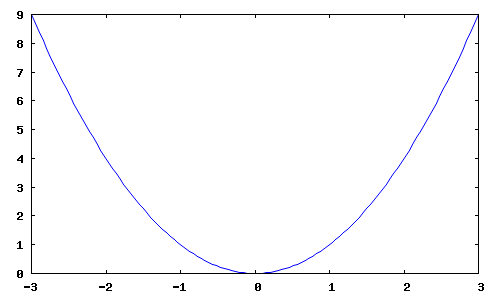
\includegraphics[width=3in]{example_0_3_1_1}

\end{exmp}

\line(1,0){60}
\linethickness{0.5mm}


\begin{exmp} Plot the points $[-3,1]$ and $[2,5]$ on a grid for $x$-range $[-10,10]$ and $y$-range $[-10,10]$. Include a label above each point.\\
${}$\\

We use \verb|point_type=7| to make closed circles and \verb|points| to list the desired points.  \verb|label| is used to create the text of each label and attach it to the desired coordinates (in this case, 1 unit above the actual points):

\begin{verbatim}
(%i3) wxdraw2d(
      grid=true,
      xrange=[-10,10],
      yrange=[-10,10],
      point_type=7,
       points([[-3,1],[2,5]]),
      label(["[-3,1]",-3,2],["[2,5]",2,6])
      );
\end{verbatim}

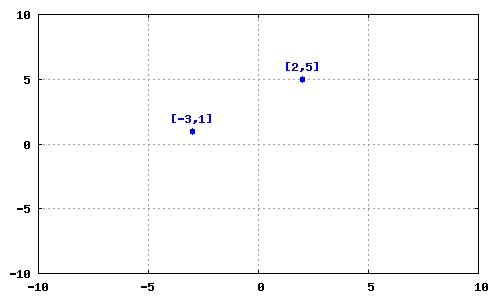
\includegraphics[width=3in]{example_0_3_2_1}

\end{exmp}

\line(1,0){60}
\linethickness{0.5mm}



\begin{exmp}  Plot a black vertical line $x=3$, and plot the unit circle in red with $x$-range $[-4,4]$ and $y$-range $[-4,4]$.  Include the $x$ and $y$ axes, a grid and a title.  \\
${}$\\

This example is a good illustration of how easily a plot can grow in complexity.  A vertical line is not a function, so it must be defined \textit{parametrically}.  We tell wxMaxima to plot many points $(3,t)$ as $t$ runs from $-4$ to $4$.  In addition, the equation of the unit circle defines a curve \textit{implicitly}:  we can't solve for $y$ in terms of $x$.  Finally, the unit circle will be distorted if we don't force the aspect ratio to be square using \verb|dimensions|:

\begin{verbatim}
(%i4) wxdraw2d(
      grid=true,
      xaxis=true,
      yaxis=true,
      dimensions=[600,600],
      xrange=[-4,4],
      yrange=[-4,4],
      title="The unit circle and the line x=3.",
      color=black,
       parametric(3,t,t,-4,4),
      color=red,
       implicit(x^2+y^2=1,x,-1,1,y,-1,1)
      ); 
\end{verbatim}

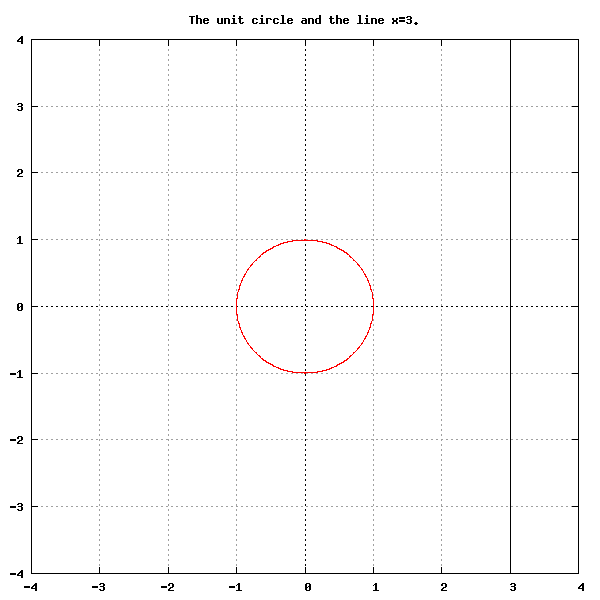
\includegraphics[width=3in]{example_0_3_3_1}

\end{exmp}

\line(1,0){60}
\linethickness{0.5mm}




\begin{exmp}  Make a quick plot of the paraboloid $z=x^2+y^2$ using \verb|wxdraw3d|.  In addition, use \verb|draw3d| to draw the paraboloid in a GNUplot window, then manipulate the plot with a mouse.\\



\begin{verbatim}
(%i5) wxdraw3d(
      explicit(x^2+y^2,x,-5,5,y,-5,5)
      );
\end{verbatim}

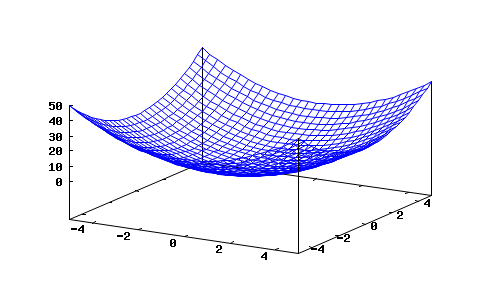
\includegraphics[width=3in]{example_0_3_4_1}

\end{exmp}

\line(1,0){60}
\linethickness{0.5mm}

\pagebreak


\section{Defining and Solving Equations}\label{Defining and Solving Equations}

In wxMaxima, the symbol ``\verb|=|'' is reserved for defining equations.  Once an equation is defined, we can use \verb|rhs| and \verb|lhs| to isolate the right and left sides.  Many equations and systems of equations can be solved using \verb|solve|, but some equations can only be solved with numerical approximations using \verb|find_root| or another approximation.

\begin{exmp} Assign the symbol \verb|EQN| to the equation $3x-6=6x+5$, then solve the equation ``manually'' by performing the usual algebraic operations to isolate $x$.  Check your answer by substituting this value of $x$ into the left and right sides of the original equation.  Finally, check your answer again by using \verb|solve|.\\
${}$\\

We run through the standard process for linear equations:

\begin{verbatim}
(%i1) EQN:3*x-6=6*x+5;
(%o1) 3*x-6=6*x+5
(%i2) %+6;
(%o2) 3*x=6*x+11
(%i3) %-6*x;
(%o3) -3*x=11
(%i4) %/-3;
(%o4) x=-11/3
\end{verbatim}

We check our answer using \verb|subst|:

\begin{verbatim}
(%i5) subst(-11/3,x,rhs(EQN));
(%o5) -17
(%i6) subst(-11/3,x,lhs(EQN));
(%o6) -17
\end{verbatim}

Finally, we repeat the solution using \verb|solve|:

\begin{verbatim}
(%i7) solve(EQN,x);
(%o7) [x=-11/3]
\end{verbatim}


\end{exmp}


\line(1,0){60}
\linethickness{0.5mm}

\begin{exmp} Attempt to solve $\ln{x}=\sin{x}$ using \verb|solve|.  What happens?  Now rephrase the problem in terms of finding a \textit{root} of another function.  Approximate the solution using \verb|find_root|.\\
${}$\\

First we attempt the naive solution, calling the equation \verb|EQN2|:

\begin{verbatim}
(%i8) EQN2:log(x)=sin(x)$
      solve(EQN2,x);
(%o9) [sin(x)=log(x)]
\end{verbatim}

wxMaxima simply repeats the question, indicating a failure to find the solution (in fact, \verb|solve| can only solve \textit{some} polynomial equations!).  However, we realize that any solution to $\ln{x}=\sin{x}$ is also a solution of $\ln{x}-\sin{x}=0$, so we can examine the function $f(x)=\ln{x}-\sin{x}$ and numerically approximate its roots.\\
${}$\\
One complication of \verb|find_root| is that we have to specify the interval on which the root occurs, and the function must be defined on the interval we choose.  We can choose an interval by quickly sketching the function:


\begin{verbatim}
(%i10) wxdraw2d(
      grid=true,
      explicit(log(x)-sin(x),x,0,10)
      );
\end{verbatim}

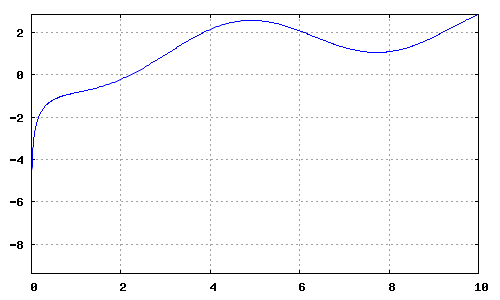
\includegraphics[width=3in]{example_0_4_2_1}

We see a root somewhere on $[2,4]$.  Note:  if we choose the interval $[0,4]$, \verb|find_root| fails because $\ln{x}$ is not defined at $x=0$!

\begin{verbatim}
(%i11) find_root(log(x)-sin(x),2,4);
(%o11) 2.219107148913746
\end{verbatim}

We obtain $x \approx 2.219$ as the numerical solution to the equation.

\end{exmp}

\line(1,0){60}
\linethickness{0.5mm}

\begin{exmp} Solve the system of equations
$\begin{cases} 2x-3y&=5 \\ 3x+y&=2 \end{cases}$ using \verb|solve|.  Plot both equations implicitly and mark the intersection point in the plot.\\

\begin{verbatim}
(%i12) L1:2*x-3*y=5$
       L2:3*x+y=2$
       solve([L1,L2],[x,y]);
(%o14) [[x=1,y=-1]]

(%i15) wxdraw2d(
       grid=true,
       color=black,
        implicit(L1,x,-2,2,y,-2,2),
        implicit(L2,x,-2,2,y,-2,2),
       color=red,
       point_type=7,
        points([[1,-1]])
       );
\end{verbatim}

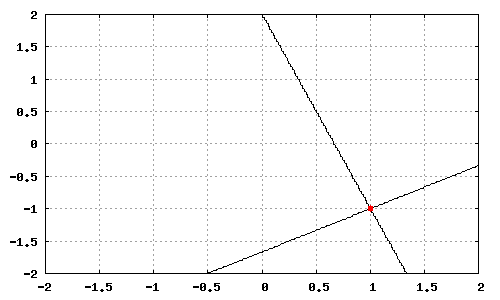
\includegraphics[width=3in]{example_0_4_3_1}

\end{exmp}


\line(1,0){60}
\linethickness{0.5mm}

\pagebreak

\section{Sequences and Sums}\label{Sequences and Sums}

\subsection{Sequences}

Sequences find a wide variety of applications, and we use them frequently in this text.  wxMaxima generates sequences using \verb|makelist| or \verb|for-do|.  \verb|makelist| offers the advantage that we can call list elements later in the calculation, while \verb|for-do| is much more flexible and powerful.

\begin{exmp} Use \verb|makelist| to generate the sequence $L=1,3,5,\dots 51$. Use wxMaxima to isolate the tenth element of the sequence. \\
${}$\\

We use the formula $2n-1$ with $n=1\dots 26$ to generate the sequence:

\begin{verbatim}
(%i1) L:makelist(2*n-1,n,1,26);
(%o1) [1,3,5,7,9,11,13,15,17,19,21,23,25,27,29,31,33,35,
        37,39,41,43,45,47,49,51]
\end{verbatim}

Now we call the tenth element of \verb|L|:

\begin{verbatim}
(%i2) L[10];
(%o2) 19
\end{verbatim}

\end{exmp}

\line(1,0){60}
\linethickness{0.5mm}


\begin{exmp} Use \verb|makelist| to generate a sequence of 20 ordered pairs on the line $y=2x$ for $x=0.0,0.1,\dots ,2$.  Feed your list of ordered pairs into \verb|wxdraw2d|. \\
${}$\\

We can generate the $x$ values using the sequence $0.1k$ for $k=0,1,\dots ,20$.  The output of \verb|makelist| is already in ``list'' form, so it is ready to feed into \verb|wxdraw2d|:

\begin{verbatim}
(%i3) POINTS:makelist([0.1*k,2*(0.1*k)],k,0,20);
(%o3) [[0,0],[0.1,0.2],[0.2,0.4],[0.3,0.6],[0.4,0.8],[0.5,1.0],
      [0.6,1.2],[0.7,1.4],[0.8,1.6],[0.9,1.8],[1.0,2.0],[1.1,2.2],
      [1.2,2.4],[1.3,2.6],[1.4,2.8],[1.5,3.0],[1.6,3.2],[1.7,3.4],
      [1.8,3.6],[1.9,3.8],[2.0,4.0]]

(%i4) wxdraw2d(
      grid=true,
      xaxis=true,
      yaxis=true,
      xrange=[-1,3],
      yrange=[-1,5],
      point_type=7,
      color=red,
      points(POINTS)
      );
\end{verbatim}

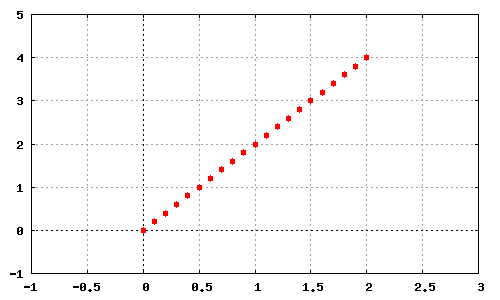
\includegraphics[width=3in]{example_0_5_2_1}

\end{exmp}

\line(1,0){60}
\linethickness{0.5mm}


\begin{exmp} Use a \verb|for-do| loop to generate the same sequence as Example 0.5.1.\\
${}$\\

When we program a \verb|for-do| loop (also called simply a ``do-loop''), we ask wxMaxima to repeat a process until some ending point is reached.  In this case, we ask wxMaxima to assign $x$ to $2n-1$ and print $x$, repeating the calculation for $n=1\dots 26$:

\begin{verbatim}
(%i5) (for n:1 thru 26 do
       (x: 2*n-1,
        print(x))
       );
       1
       3
       5
       7
       9
       11
       13
       15
       17
       19
       21
       23
       25
       27
       29
       31
       33
       35
       37
       39
       41
       43
       45
       47
       49
       51
       
(%o5)  done
\end{verbatim}

\end{exmp}

\line(1,0){60}
\linethickness{0.5mm}

\begin{exmp} The Fibonacci sequence is defined by a recursive formula $f_n=f_{n-1}+f_{n-2}$; that is, the next number is obtained by adding the previous two numbers.  If we start the sequence with $0,1,\dots$, the entire sequence is given by $0,1,1,2,3,5,8,\dots$.  Use a do-loop to generate the first twenty terms of the Fibonacci sequence.\\
${}$\\

Our use of \verb|for-do| is more substantial in this example:  we have to repeat a calculation several times and use the output of each step to compute the next step.  We define the two starting numbers $f_{n-1}$ and $f_{n-2}$ first, then the loop prints the next Fibonacci number $X$, changes the ${(n-1)}^{\mathrm{th}}$ term to the ${(n-2)}^{\mathrm{th}}$ term and assigns the ${(n-1)}^{\mathrm{th}}$ term to $X$.  Then the process is repeated 18 times for a total of 20 Fibonacci numbers.

\begin{verbatim}
(%i6) N_1:1$
      N_2:0$
(%i8) 
      (for i:1 thru 18 do
       (X:N_2+N_1,
        print(X),
        N_2:N_1,
        N_1:X)
       );
       1
       2
       3
       5
       8
       13
       21
       34
       55
       89
       144
       233
       377
       610
       987
       1597
       2584
       4181
       
(%o8)  done
\end{verbatim}


\end{exmp}

\line(1,0){60}
\linethickness{0.5mm}
${}$\\

\subsection{Sums}

wxMaxima computes sums using \verb|sum|.  The notation is very close to sigma notation:

\begin{exmp} Use \verb|sum| to compute the sum $2+4+6+\dots +50$.\\
${}$\\

In sigma notation, the sum is written $\sum_{n=1}^{25} 2n$, and the arguments of \verb|sum| simply refer to all the parts of this notation:

\begin{verbatim}
(%i9) sum(2*n,n,1,25);
(%o9) 650
\end{verbatim}

\end{exmp}

\line(1,0){60}
\linethickness{0.5mm}

\begin{exmp}  Find an algebraic formula for the sum $1+2+\dots +n$, then use a substitution to obtain the sum of the first 100 natural numbers.\\
${}$\\

In sigma notation, we wish to compute $\sum_{k=1}^n k$.  The classic formula is obtained using \verb|sum| followed by \verb|simpsum|, then we substitute $n=100$:

\begin{verbatim}
(%i10) sum(k,k,1,n),simpsum;
(%o10) (n^2+n)/2
(%i11) subst(100,n,%);
(%o11) 5050
\end{verbatim}

\end{exmp}

\line(1,0){60}
\linethickness{0.5mm}
\pagebreak

\section{Application: Line Passing Through Two Given Points}\label{Application:  Line Passing Through Two Given Points}

As a demonstration of the utility of symbolic calculation, we design a function to quickly plot the line connecting two points.\\
${}$\\
\begin{exmp}  Create a function \verb|LINE(a,b,c,d,x)| that computes the equation of a line passing through the points $(a,b)$ and $(c,d)$.  Set up your code so the simple assignment of $a,b,c,d$ will immediately produce a nice plot of the line and the two given points.  Apply your code to the points $(-0.51,-3.47)$ and $(7.12,3.94)$.\\
${}$\\


First, we define each point as a function of two variables.  The output of each function is in the correct form to use as a point within \verb|wxdraw2d|.  Then we compute the slope between the points as a function of all four variables:\\

\begin{verbatim}
(%i1) POINT1(a,b):=[a,b]$
      POINT2(c,d):=[c,d]$
      SLOPE(a,b,c,d):=(d-b)/(c-a)$  
\end{verbatim}

The next step is to plug into the point-slope formula $y-y_0=m(x-x_0)$ and solve for $y$ as a function of $x$.  We use \verb|POINT1| as $(x_0,y_0)$.
           
\begin{verbatim}           
(%i4) LINE(a,b,c,d,x):=SLOPE(a,b,c,d)*(x-a)+b$
\end{verbatim}

Finally, we make the assignments for $a,b,c,d$ and set up \verb|wxdraw2d|.  Note that everything remains general within \verb|wxdraw2d|, so we can plot the line between any two points immediately by making new assignments for $a,b,c,d$:

\begin{verbatim}
(%i5) a:-.51$
      b:-3.47$
      c:7.12$
      d:3.94$

      wxdraw2d(
      grid=true,
      xaxis=true,
      yaxis=true,
      color=black,
       explicit(LINE(a,b,c,d,x),x,a-1,c+1),
      color=red,
      point_type=7,
      points([[a,b],[c,d]])
      );
\end{verbatim}

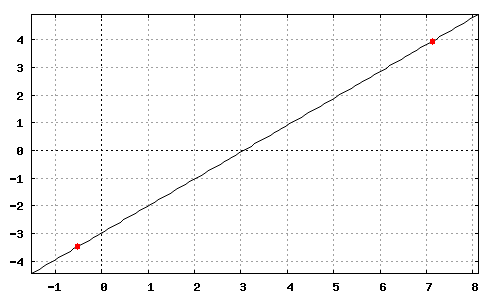
\includegraphics[width=3in]{example_0_6_1_1}
${}$\\


\end{exmp}

\line(1,0){60}
\linethickness{0.5mm}

\pagebreak






\section{Module 0 Exercises}\label{Module 0 Exercises}

\begin{enumerate}

\item  Define the expressions $A=\sqrt{3}$ and $B=5$, then find decimal approximations for $A+B$ and $A/B$.

\item  Define expressions $A=x^2$ and $B=e^x$.  Substitute $B$ for $x$ in the formula for $A$, then evaluate the resulting expression at $x=0.1$ and obtain a decimal approximation.

\item  Use \verb|trigexpand| to find a formula for $\sin{(x+y)}$ in terms of $\sin{x}$, $\sin{y}$, $\cos{x}$ and $\cos{y}$.  Use your result to compute $\sin{\frac{5\pi}{12}}$ by using the fact that $\frac{5\pi}{12}=\frac{\pi}{6}+\frac{\pi}{4}$.  Re-calculate $\sin{\frac{5\pi}{12}}$ directly and use \verb|float| to verify your answer.


\item  Add and simplify:  $\frac{2x^2-x-6}{x^2-9}+\frac{x^3-x^2-4x+4}{x^2+5x+6}$.  Express your answer in factored form.

\item Solve the equation $ax^2+bx+c=0$ for $x$.  


\item Make a plot of $f(x)=\sin{(\ln{x})}-0.2$ on $[10,30]$ including the x-axis.  Use \verb|find_root| to approximate the solution of $\sin{(\ln{x})}=0.2$ on this interval.  Verify your answer by evaluating $\sin{(\ln{x})}$ at the value of $x$ you found.

\item  Define $f(x)=x+2$ and $g(x)=x^2$.  Find the intersections of these two curves, then make a plot of both functions including the intersection points as closed circles.  Label each intersection point using decimal coordinates rounded to the second decimal place.

\item  Use \verb|makelist| and \verb|for-do| to generate the first thirty terms of the sequence $1,\frac{1}{2},\frac{1}{4},\dots$.

\item  The recursive formula for a sequence is given by $f_n=2f_{n-1}$ with a starting point of $f_0=3$.  Use a do-loop to generate the first 10 terms of this sequence recursively (as in Example 0.5.4).  Once the sequence is written down, you can guess an explicit formula for $f_n$.  Once you find this formula, use \verb|makelist| to generate the same sequence.

\item Use \verb|makelist| to plot 40 circles centered at the origin with radii $0.1,0.2,0.3,\dots$ in a single plot.  This problem is tricky because your list must produce elements that \verb|wxdraw2d| understands:  \verb|implicit| and its proper arguments must be included with each list element!

\item Any parabola can be written $f(x)=ax^2+bx+c$.  The parameters $a,b,c$ completely define the parabola.  If you are given three points lying on an unknown parabola, they generate a system of three equations in $a,b,c$.  \verb|solve| can quickly produce the solution of this system.  The proper syntax is \verb|solve([eqn1,eqn2,eqn3],[var1,var2,var3])|.  Write a solution similar to Example 0.6.1 to take any three points and produce a plot of the points together with the parabola passing through them.  Apply your code to the points $(-6.8,-5.5)$, $(0.1,6.7)$ and $(3.2,-0.9)$.



\end{enumerate}





\chapter{Classical Integration Techniques}

\vspace*{\fill}

\minitoc

\vspace*{\fill}


\flushleft{\textbf{\Large Key Commands Included in This Module}}
\newline
\newline

\begin{tabular}{l l l l l}
 \verb|integrate   |   &\verb|diff   |   &\verb|ratprint   |  &\verb|sublis   |   &\verb|trigexpand   |\\
 \verb|float  |   &\verb|kill(all)   |   &\verb|logcontract   |  &\verb|divide  |   &\verb|dimensions   |\\
 \verb|filled_func   |   &\verb|solve   |   &\verb|factor   |  &\verb|partfrac   |   &\verb|declare   |\\
 \verb|wxdraw2d    |   &\verb|coeff   |   &\verb|denom   |   &\verb|limit   |  &\verb|   |\\
 \verb|subst   |   &\verb|trigsimp   |   &\verb|ratsimp   |   &\verb|trigreduce   |  &\verb|   |\\
\end{tabular}



\pagebreak
\section{Quick Integration Review}\label{Quick Integration Review}

\subsection{Definite Integrals}
The notion of integration arises from \textit{The Area Problem}: the problem of computing the signed area bounded by a function $f(x)$ on an interval $[a,b]$.  The area problem is usually introduced by splitting the interval $[a,b]$ into many small sub-intervals and approximating each ``slice'' of area with a rectangle.  The resulting approximation is called a Riemann Sum (in the next module we will explore numerical approximations in more detail).  The \textit{exact} area bounded on $[a,b]$ can be defined as a limit of a Riemann sum as the rectanglular slices become arbitrarily narrow, and we say the area is given by the \textbf{definite integral}: \[A=\displaystyle \int_a^b f(x)\ \mathrm{d}x\]  \\
wxMaxima computes definite integrals using the \verb|integrate| command.\\

${}$\\

\begin{exmp} Compute $\displaystyle \int_{-1}^{2} \frac{1}{1+x^2} \ \mathrm{d}x$ and produce a plot of $f(x)$ together with the shaded area you have computed.\\
${}$\\

We define $f(x)$ as a function, apply \verb|integrate|, and use \verb|float| to obtain a decimal approximation:

\begin{verbatim}
(%i1) f(x):=1/(1+x^2)$
(%i2) integrate(f(x),x,-1,2);
(%o2) atan(2)+%pi/4
(%i3) float(%);
(%o3) 1.892546881191539
\end{verbatim}

We see that $\displaystyle \int_{-1}^{2} \frac{1}{1+x^2} \ \mathrm{d}x = \tan^{-1}(2) + \frac{\pi}{4} \approx 1.89$.\\
${}$\\

To produce the shaded plot, we have to use \verb|filled_func|, which expects us to define the area \textit{between} two curves (we use $y=0$ as the second curve).  We set a variety of options inside \verb|wxdraw2d| to produce a nice plot:

\begin{verbatim}
(%i4) load(draw)$
(%i5) wxdraw2d(
      grid=true,
      xaxis=true,
      yaxis=true,
      xrange=[-5,5],
      yrange=[-.2,1.2],
      title="Area bounded by f(x) on [-1,2]",
      color=black,
       explicit(f(x),x,-5,5),
      filled_func=true,
       filled_func=f(x),
       explicit(0,x,-1,2),
      filled_func=false
      ); 
\end{verbatim}

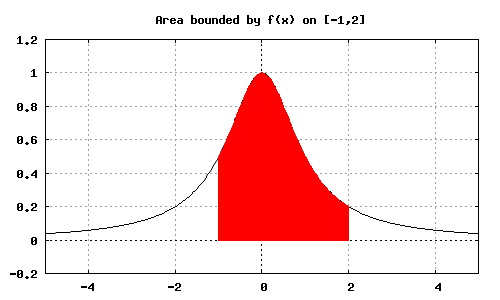
\includegraphics[width=3in]{example_1_1_1_1}

\end{exmp}

\line(1,0){60}
\linethickness{0.5mm}


\subsection{Area Functions}

An \textbf{area function} is a definite integral with a variable limit of integration.  For example, to find the area bounded by $f$ on $[a,x]$, we write: \[A(x)=\displaystyle \int_a^x f(t)\ \mathrm{d}t\]\\

where $t$ is introduced as a ``dummy variable'' since $x$ is already used to denote the endpoint of the integration interval.  \\

${}$\\

\begin{exmp} Define the area function $A(x)=\displaystyle \int_1^x \sin{x} \ \mathrm{d} x$.  Plot the areas represented by $A(\frac{\pi}{2})$ and $A(\pi)$.  Use a difference of area functions to compute the area bounded by $f(x)=\sin{x}$ on $[\frac{\pi}{2},\pi]$, and verify your answer using \verb|integrate| directly.\\

${}$\\

First, we define $A(x)$ in terms of the dummy variable, $t$:

\begin{verbatim}
(%i6) A(x):=integrate(sin(t),t,1,x);
\end{verbatim}
\verb|(%o6) | $A(x):=\displaystyle \int_1^x \sin{t} \ \mathrm{d}t$\\

${}$\\

Now we can make the shaded plots.  $A(\frac{\pi}{2})=\displaystyle \int_1^{\frac{\pi}{2}} \sin{t} \ \mathrm{d}t$, so we simply shade in the area bounded by $\sin{t}$ on $[1,\frac{\pi}{2}]$.  Similarly, the shaded area for $A(\pi)$ is just the bounded area on $[1,\pi]$:

\begin{verbatim}
(%i7) wxdraw2d(
      grid=true,
      xaxis=true,
      yaxis=true,
      xrange=[0,4],
      yrange=[-1.5,1.5],
      title="Shaded area given by A(pi/2)",
      color=black,
       explicit(sin(x),x,0,4),
      filled_func=true,
       filled_func=sin(x),
       explicit(0,x,1,%pi/2),
      filled_func=false
      );
 
(%i8) wxdraw2d(
      grid=true,
      xaxis=true,
      yaxis=true,
      xrange=[0,4],
      yrange=[-1.5,1.5],
      title="Shaded area given by A(pi)",
      color=black,
       explicit(sin(x),x,0,4),
      filled_func=true,
       filled_func=sin(x),
       explicit(0,x,1,%pi),
      filled_func=false
      );
\end{verbatim} 


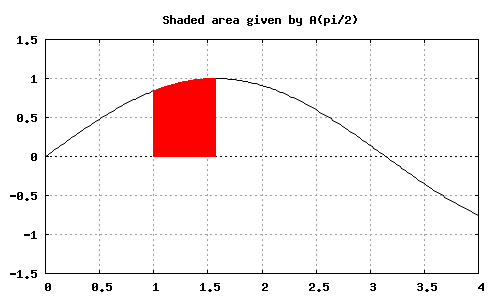
\includegraphics[width=2.7in]{example_1_1_2_1}
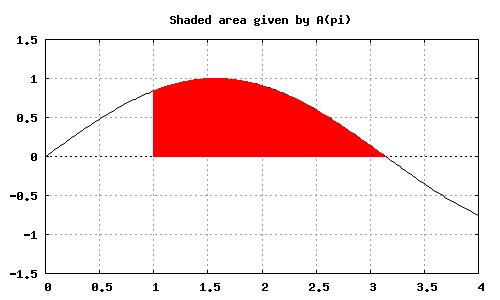
\includegraphics[width=2.7in]{example_1_1_2_2}
${}$\\

It is clear from the graphs that the area bounded on $[\frac{\pi}{2},\pi]$ is just the difference in the two areas $A(\pi)-A(\frac{\pi}{2})$.  It is also apparent that the ``starting point'' $x=1$ makes no difference in the calculation.  Finally, we compute the area in two different ways:

\begin{verbatim}
(%i9) A(%pi)-A(%pi/2);
(%o9) 1

(%i10) integrate(sin(x),x,%pi/2,%pi);
(%o10) 1
\end{verbatim}


\end{exmp}

\line(1,0){60}
\linethickness{0.5mm}
\pagebreak

\subsection{The Fundamental Theorem of Calculus}

The Fundamental Theorem of Calculus (FTC) is motivated geometrically by the idea that a ``thin slice'' of area bounded on $[x,x+h]$ may be computed in two different ways:  as a rectanglular approximation $f(x)\cdot h$ or as a difference of area functions $A(x+h)-A(x)$.  When we equate these two representations of area and take the limit $h \to 0$, we obtain:
\[f(x)\cdot h=A(x+h)-A(x) \implies f(x)=\lim_{h \to 0} \frac{A(x+h)-A(x)}{h} = A'(x)\]

In other words, the area function is the \textit{antiderivative} of the curve that bounds the area.\\
${}$\\
The FTC tells us that we can compute the definite integral $\displaystyle \int_a^b f(x) \ \mathrm{d}x$ by guessing an antiderivative of $f(x)$ (an area function $A(x)$) and evaluating it across the endpoints of the interval to obtain $A(b)-A(a)$.  We don't have to worry about the arbitrary constant in the antiderivative, since it cancels in the difference.  Note that the \textbf{indefinite integral} $\displaystyle \int f(x) \ \mathrm{d}x$ is a synonym for the antiderivative of $f(x)$, and wxMaxima computes antiderivatives by using \verb|integrate| with no limits of integration. \\



\begin{exmp}  Use the FTC to compute the area $\displaystyle \int_{\frac{\pi}{2}}^{\pi} \sin{x}\ \mathrm{d}x$ from Example 1.1.2.\\
${}$\\


We use \verb|integrate| to quickly compute an antiderivative, $F(x)$.  Note that \verb|''(%)| is necessary to assign a \textit{function} to a previous output. 

\begin{verbatim}
(%i11) f(x):=sin(x)$
       integrate(f(x),x);
(%o12) -cos(x)
(%i13) F(x):=''(%);
(%o13) F(x):=-cos(x)
(%i14) F(%pi)-F(%pi/2);
(%o14) 1
\end{verbatim}

We get the same answer we obtained by using a difference of area functions in Example 1.1.2.

\line(1,0){60}
\linethickness{0.5mm}

\end{exmp}



\begin{exmp}  Compute $\displaystyle \int_1^3 \frac{1}{x^2} \ \mathrm{d}x$ by finding the antiderivative of $\frac{1}{x^2}$ and evaluating it across the endpoints of the integration interval. Verify your answer by directly computing the definite integral.\\
${}$\\
To illustrate a slightly different approach to the problem, we define the antiderivative as an expression and use \verb|subst| to evaluate it across the endpoints.

\begin{verbatim}
(%i15) A:integrate(1/x^2,x);
(%o15) -1/x
(%i16) subst(3,x,A)-subst(1,x,A);
(%o16) 2/3

(%i17) integrate(1/x^2,x,1,3);
(%o17) 2/3
\end{verbatim}



\end{exmp}

\line(1,0){60}
\linethickness{0.5mm}
\pagebreak



\pagebreak
\section{Transforming Integrals With Substitutions}\label{Transforming Integrals With Substitutions}

\subsection{\textit{u}-Substitution}

To make a \textit{u}-substitution, we define a variable \textit{u} in terms of \textit{x} (and $\mathrm{d}u$ in terms of $\mathrm{d}x$), so that 
$$\int f(x)\ \mathrm{d}x=\int g(u)\ \mathrm{d}u$$
where it is understood that it is easier to guess the antiderivative $G(u)$.  Once $G(u)$ is determined, we use the definition of $u$ to transform back to the antiderivative $F(x)$.  $u$-substitution can also be applied to definite integrals, where we can either evaluate $F(x)$ across the original integration limits or transform the integration limits in terms of $u$.\\
${}$\\

While any substitution technique is really intended for ``pencil-and-paper'' integration, the process can teach us a lot about symbolic manipulation within wxMaxima.  To perform a \textit{u}-substitution, we:

\begin{enumerate}

\item Decide on a substitution and use \verb|diff| to produce the differential $\mathrm{d}u$ (called \verb|del(u)|) in wxMaxima), then express $\mathrm{d}x$ in terms of $\mathrm{d}u$ using \verb|solve|. 

\item Extract the resulting equation  using \verb|%[1]| and replace \verb|del(x)| with its expression in terms of \verb|del(u)| in the integrand.

\item Use \verb|subst| to transform the entire integrand in terms of $u$, then perform the integral, remembering that \verb|integrate| expects only the \textit{coefficient} of \verb|del(u)|.

\item Substitute the definition of $u$ in terms of $x$ into the resulting antiderivative.  Alternatively, in a  definite integral we can choose to transform the limits of integration in terms of $u$ before evaluation.

\end{enumerate}

${}$\\

\begin{exmp} Use the substitution $u=x^2$ to compute $\displaystyle \int 5x\cdot \sin{(x^2)}\ \mathrm{d}x$.  Verify your answer using \verb|diff|.\\

${}$\\


\begin{verbatim}
(%i1) INTEGRAND:(5*x)*sin(x^2)*del(x)$

(%i2) solve(diff(u)=diff(x^2),del(x));
(%o2) [del(x)=del(u)/(2*x)]
(%i3) %[1];
(%o3) del(x)=del(u)/(2*x)

(%i4) subst(rhs(%),del(x),INTEGRAND);
(%o4) (5*sin(x^2)*del(u))/2
(%i5) subst(u,x^2,%);
(%o5) (5*sin(u)*del(u))/2
\end{verbatim}

The integral is now expressed entirely in terms of $u$ as $\displaystyle \frac{5}{2} \int \sin{u}\ \mathrm{d}u$, which is easy enough to guess.  For the sake of completeness we use wxMaxima to compute the integral, then we transform the result to a function of the original variable, $x$:\\
${}$\\

\begin{verbatim}
(%i6) integrate(coeff(%,del(u)),u);
(%o6) -(5*cos(u))/2

(%i7) subst(x^2,u,%);
(%o7) -(5*cos(x^2))/2
\end{verbatim}

We conclude that $\displaystyle \int 5x\cdot \sin{(x^2)}\ \mathrm{d}x=-\frac{5}{2}\cos{(x^2)}+C$.  Checking our answer with \verb|diff|:

\begin{verbatim}
(%i8) diff(%,x);
(%o8) 5*x*sin(x^2)
\end{verbatim}

We see that the chain rule produces the necessary factor of $x$, and the constant is set up to work out to $5$.

\end{exmp}

\line(1,0){60}
\linethickness{0.5mm}




\begin{exmp} Compute $\displaystyle \int_{-1}^{0} \frac{x}{\sqrt{1-x}}\ \mathrm{d}x$ by making the substitution $u=1-x$.\\

${}$\\

First, we find the indefinite integral in terms of $u$:

\begin{verbatim}
(%i9) kill(all)$
(%i1) INTEGRAND:(x/(sqrt(1-x)))*del(x)$
(%i2) solve(diff(u)=diff(1-x),del(x));
(%o2) [del(x)=-del(u)]
(%i3) %[1];
(%o3) del(x)=-del(u)
(%i4) subst(rhs(%),del(x),INTEGRAND);
(%o4) -(x*del(u))/sqrt(1-x)
(%i5) solve(u=1-x,x);
(%o5) [x=1-u]
(%i6) subst(rhs(%[1]),x,(%o13));
(%o6) -((1-u)*del(u))/sqrt(u)
\end{verbatim}

The integrand $-\frac{1-u}{\sqrt{u}}\ \mathrm{d}u$ is simple to integrate using the standard ``power rule'' for antiderivatives; that is, the $u$ substitution appropriately results in a ``guessable'' antiderivative.  For convenience, we use wxMaxima to find the antiderivative, then we label it as $G(u)$:

\begin{verbatim}
(%i7) integrate(coeff(%,del(u)),u);
(%o7) (2*u^(3/2)-6*sqrt(u))/3
(%i8) G(u):=''(%);
(%o8) G(u):=(2*u^(3/2)-6*sqrt(u))/3
\end{verbatim}

We finish the definite integral by transforming back to $x$ and evaluating across the original limits of integration.   \\

\begin{verbatim}
(%i9) G(1-x);
(%o9) (2*(1-x)^(3/2)-6*sqrt(1-x))/3
(%i10) F(x):=''(%);
(%o10) F(x):=(2*(1-x)^(3/2)-6*sqrt(1-x))/3
(%i11) F(0)-F(-1);
(%o11) 2^(3/2)/3-4/3
\end{verbatim}

Alternatively, we can transform the limits of integration in terms of $u$:\\

\begin{verbatim}
(%i12) u(x):=1-x$
       u_lower:u(-1);
       u_upper:u(0);
(%o13) 2
(%o14) 1
(%i15) G(u_upper)-G(u_lower);
(%o15) 2^(3/2)/3-4/3
\end{verbatim}


\end{exmp}

\line(1,0){60}
\linethickness{0.5mm}
${}$\\

\subsection{Trigonometric Substitution}

A trigonometric substitution is used when we recognize a troublesome expression in the integrand that may simplify according to one of the pythagorean identities:  $\sin^2{x}+\cos^2{x}=1$ or $\tan^2{x}+1=\sec^2{x}$.\\

${}$\\

Like $u$-substitutions, trigonometric substitutions are intended for pencil and paper calculations, but performing a trigonometric substitution within wxMaxima is still instructive.
${}$\\
${}$\\
\begin{exmp} Compute $\displaystyle \int_{-0.5}^{0.5} \frac{1}{\sqrt{1-x^2}}\ \mathrm{d}x$ by using a trigonometric substitution.\\
${}$\\
We choose the substitution $x=\sin{t}$ to take advantage of the fact that $1-\sin^2{t}=\cos^2{t}$.  Note that the trigonometric substitution comes with an implicit domain:  to uniquely cover all possible values of $\sin{t}$, we work in the domain $[-\frac{\pi}{2},\frac{\pi}{2}]$.  There is no loss of generality in this domain restriction because the integrand is only defined for $x$ values on $[-1,1]$, and all these values are covered by $\sin{t}$ on $[-\frac{\pi}{2},\frac{\pi}{2}]$.

\begin{verbatim}
(%i16) kill(all)$
(%i1) INTEGRAND:(1/sqrt(1-x^2))*del(x);
(%o1) del(x)/sqrt(1-x^2)
(%i2) solve(diff(x)=diff(sin(t)),del(x));
(%o2) [del(x)=cos(t)*del(t)]
(%i3) subst(rhs(%[1]),del(x),INTEGRAND);
(%o3) (cos(t)*del(t))/sqrt(1-x^2)
(%i4) subst(sin(t),x,%);
(%o4) (cos(t)*del(t))/sqrt(1-sin(t)^2)
(%i5) trigsimp(%);
(%o5) (cos(t)*del(t))/abs(cos(t))
\end{verbatim}

We have to intervene manually because wxMaxima cannot perform integrals containing absolute values.  With $t$ restricted to $[-\frac{\pi}{2},\frac{\pi}{2}]$, $\cos{t}$ is always positive, so $|\cos{t}|=\cos{t}$.  The integrand simplifies to $1\cdot \mathrm{d}t$.  The integral evaluates to $G(t)=t$, and we substitute the expression for $t$ in terms of $x$ to obtain the antiderivative $F(x)$:

\begin{verbatim}
(%i6) G:integrate(1,t);
(%o6) t
(%i7) solve(x=sin(t),t);
      solve: using arc-trig functions to get a solution.
      Some solutions will be lost.
(%o7) [t=asin(x)]
(%i8) subst(rhs(%[1]),t,G);
(%o8) asin(x)
(%i9) F(x):=''(%)$
\end{verbatim}

We ignore the \verb|solve| warning, because $t$ lies on the standard domain $[-\frac{\pi}{2},\frac{\pi}{2}]$.  We finish by evaluating $F(x)$ across the integration limits:

\begin{verbatim}
(%i10) F(.5)-F(-.5);
(%o10) 1.047197551196598
\end{verbatim}

We suppress a string of warnings using \verb|ratprint|, and check our answer with \verb|integrate|:

\begin{verbatim}
(%i11) ratprint:false$
(%i12) integrate(1/sqrt(1-x^2),x,-.5,.5);
(%o12) 1.047197551196598
\end{verbatim}

\end{exmp}

\line(1,0){60}
\linethickness{0.5mm}

\begin{exmp} Compute $\displaystyle \int \frac{1}{x\sqrt{3+x^2}}\ \mathrm{d}x$ by using a trigonometric substitution.\\
${}$\\

The square root contains an expression that is \textit{close} to $1+\tan^2{x}$, but we need the substitution for $x^2$ to produce a factor of $3$ so it can be factored out of the square root. We choose the substitution $x=\sqrt{3} \tan{t}$.  Again, we are working with an implicit domain of $[-\frac{\pi}{2},\frac{\pi}{2}]$ for $t$, this time corresponding to a domain of $[-\infty,\infty]$ for $x=\sqrt{3} \tan{t}$.

\begin{verbatim}
(%i13) kill(all)$
(%i1) INTEGRAND:(1/(x*sqrt(3+x^2)))*del(x);
(%o1) del(x)/(x*sqrt(x^2+3))
(%i2) solve(diff(x)=diff(sqrt(3)*tan(t)),del(x));
(%o2) [del(x)=sqrt(3)*sec(t)^2*del(t)]
(%i3) subst(rhs(%[1]),del(x),INTEGRAND);
(%o3) (sqrt(3)*sec(t)^2*del(t))/(x*sqrt(x^2+3))
(%i4) subst(sqrt(3)*tan(t),x,%);
(%o4) (sec(t)^2*del(t))/(tan(t)*sqrt(3*tan(t)^2+3))
(%i5) trigsimp(%);
(%o5) (abs(cos(t))*del(t))/(sqrt(3)*cos(t)*sin(t))
\end{verbatim}

Again, we must intervene manually to cancel the factor of $\cos{t}$ because wxMaxima doesn't recognize that $\cos{t}$ is always positive on the implicit domain.\\

\begin{verbatim}
(%i6) G:integrate(1/(sqrt(3)*sin(t)),t);
(%o6) (log(cos(t)-1)/2-log(cos(t)+1)/2)/sqrt(3)    
\end{verbatim}

Finally, we substitute $t$ into the last expression to get the antiderivative in terms of $x$.  Note  that the \verb|solve| warning can be ignored once again because we are implicitly working on the standard restricted domain of the tangent function:\\

\begin{verbatim}
(%i7) solve(x=sqrt(3)*tan(t),t);
      solve: using arc-trig functions to get a solution.
      Some solutions will be lost.
(%o7) [t=atan(x/sqrt(3))]
(%i8) subst(rhs(%[1]),t,G);
(%o8) (log(1/sqrt(x^2/3+1)-1)/2-log(1/sqrt(x^2/3+1)+1)/2)/sqrt(3)
(%i9) logcontract(%);
\end{verbatim}

\verb|(%o9)  | $\displaystyle \frac{\log \left( -\frac{\sqrt{x^2+3}-\sqrt{3}}{\sqrt{x^2+3}+\sqrt{3}}\right)} {2\cdot \sqrt{3}}$\\
${}$\\
This answer agrees with the standard integration tables within a minus sign in the argument of \verb|log| (wxMaxima generally ignores the absolute values in this sort of antiderivative).

\end{exmp}

\line(1,0){60}
\linethickness{0.5mm}
\pagebreak



\section{More Integration Techniques}\label{More Integration Techniques}


\subsection{Integration by Parts}

Integration by parts is a ``pencil and paper'' method used to integrate a product of two functions. A short-hand derivation of the formula is given below, starting with the product rule for derivatives:


\verb|                             |  $(uv)'=u'v+uv'$\\
${}$\\
\verb|                         |  $\implies$  $uv'=(uv)'-u'v$\\
${}$\\
\verb|                         |  $\implies$ 	 $u\cdot \mathrm{d}v=(uv)'\cdot \mathrm{d}x-v\cdot \mathrm{d}u$\\
${}$\\
\verb|                         |  $\implies$  $\displaystyle \int u\ \mathrm{d}v = uv - \displaystyle \int v\ \mathrm{d}u$\\
${}$\\

The definite integral version is discussed in the Exercises.  When we solve an integral using integration by parts, we have to choose the function $u$ and the differential $\mathrm{d}v$ so that $\mathrm{d}u$ is \textit{simpler} than $u$, and $v$ is relatively easy to compute from $\mathrm{d}v$.  \\
${}$\\


\begin{exmp}  Compute $\displaystyle \int x\cdot \sin{x}\ \mathrm{d}x$ using integration by parts.  Check your answer using \verb|diff|.\\
${}$\\
We choose $u=x$ ($\mathrm{d}u$ is clearly $\mathrm{d}x$) and $dv=\sin{x}\cdot \mathrm{d}x$, then find $v$ in wxMaxima by computing $\displaystyle \int  \mathrm{d}v$:

\begin{verbatim}
(%i1) u:x;
      v:integrate(sin(x),x);
(%o1) x
(%o2) -cos(x)
(%i3) u*v-integrate(v,x);
(%o3) sin(x)-x*cos(x)
\end{verbatim}

Finally, we check our answer using \verb|diff|:

\begin{verbatim}
(%i4) diff(%,x);
(%o4) x*sin(x)
\end{verbatim}

\end{exmp}

\line(1,0){60}
\linethickness{0.5mm}


\begin{exmp}  Compute $\displaystyle \int x^2\cdot \sin{x}\ \mathrm{d}x$ using two iterations of integration by parts.  Check your answer using \verb|diff|.\\

${}$\\

We choose $u_1=x^2$ and $\mathrm{d}v_1=\sin{x}\cdot \mathrm{d}x$:

\begin{verbatim}
(%i5) u1:x^2$
      diff(u1);
      v1:integrate(sin(x),x);
(%o6) 2*x*del(x)
(%o7) -cos(x)

(%i8) TERM1:u1*v1;
      INTEGRAND1:v1*diff(u1);
(%o8) -x^2*cos(x)
(%o9) -2*x*cos(x)*del(x)
\end{verbatim}

The first parts iteration is complete, yielding $-x^2\cdot \cos{x} -\displaystyle \int -2x\cdot \cos{x}\ \mathrm{d}x$.  Now we choose $u_2=-2x$ and $dv_2=\cos{x}\cdot \mathrm{d}x$ to perform the second integration by parts:

\begin{verbatim}
(%i10) u2:-2*x$
       diff(u2);
       v2:integrate(cos(x),x);
(%o11) -2*del(x)
(%o12) sin(x)

(%i13) TERM2:u2*v2;
       INTEGRAND2:v2*diff(u2);
(%o13) -2*x*sin(x)
(%o14) -2*sin(x)*del(x)
\end{verbatim}

The second parts integration yields $-2x\cdot \sin{x} - \displaystyle \int -2\sin{x}\ \mathrm{d}x$. Finally, we put together the final result:  $u_1\cdot v_1-\left(u_2\cdot v_2-\displaystyle \int v_2\ \mathrm{d}u_2\right)$ and check using \verb|diff|:

\begin{verbatim}
(%i15) TERM1-(TERM2-integrate(coeff(INTEGRAND2,del(x)),x));
(%o15) 2*x*sin(x)-x^2*cos(x)+2*cos(x)

(%i16) diff(%,x);
(%o16) x^2*sin(x)
\end{verbatim}

\end{exmp}

\line(1,0){60}
\linethickness{0.5mm}


\subsection{Partial Fractions Decomposition}

Partial fractions decomposition is used to break a rational integrand into smaller pieces, each of which has a simple antiderivative.   Assuming the degree of $P(x)$ is less than the degree of $Q(x)$ in the rational expression $\frac{P(x)}{Q(x)}$, we can factor the denominator into linear and irreducible quadratic factors, say $Q(x)=D_1(x)\cdot D_2(x)\cdots D_n(x)$, then express $\frac{P(x)}{Q(x)}$ as a sum of simpler fractions, each with a $D_i$ (or possibly a power of $D_i$) for its denominator. If the degree of $P(x)$ is greater than or equal to the degree of $Q(x)$, then we simply start the decomposition by performing polynomial long division.\\
${}$\\
There are a variety of cases to consider in order to express the decomposition with sufficient generality.  We assign unknown numerators $N_i$ to each of the fractions in the decomposition according to the following rules:\\

\begin{enumerate}
\item Each linear denominator must have a constant numerator, and each irreducible quadratic denominator must have a linear numerator.

\item If a repeated factor $D_i^n$ appears in the factorization of $Q(x)$, then the decomposition must contain fractions with denominators $D_i,D_i^2,\dots ,D_i^n$ each containing numerators according to 1.
\end{enumerate}


Once the decomposition is proposed, we can solve for the $N_i$'s algebraically by constructing a system of equations.  The resulting rational expressions $\frac{N_i}{D_i}$ can all be integrated quickly, requiring at most a $u$-substitution.\\

${}$\\
\begin{exmp} Compute the partial fractions decomposition of $\frac{x-4}{3x^3+5x^2+4x+2}$ by performing the algebra step-by-step.\\
${}$\\
We start by factoring the denominator and proposing the partial fractions decomposition as an equation:

\begin{verbatim}
(%i17) kill(all)$
(%i1) R:(x-4)/(3*x^3+5*x^2+4*x+2)$
      factor(denom(R));
(%o2) (x+1)*(3*x^2+2*x+2)
(%i3) EQN:R=(A/(x+1))+(B*x+C)/(3*x^2+2*x+2);
(%o3) (x-4)/(3*x^3+5*x^2+4*x+2)=(C+x*B)/(3*x^2+2*x+2)+A/(x+1)
\end{verbatim}

Now we multiply both sides of the equation by the original denominator, expand the result to a polynomial and produce a list of equations by comparing the coefficients of each power of $x$ on the left and right sides:

\begin{verbatim}
(%i4) EQN*(denom(R));
(%o4) x-4=(3*x^3+5*x^2+4*x+2)*((C+x*B)/(3*x^2+2*x+2)+A/(x+1))
(%i5) ratsimp(%);
(%o5) x-4=(x+1)*C+(x^2+x)*B+(3*x^2+2*x+2)*A
(%i6) expand(%);
(%o6) x-4=x*C+C+x^2*B+x*B+3*x^2*A+2*x*A+2*A
(%i7) EQN1:coeff(lhs(%o6),x,2)=coeff(rhs(%o6),x,2);
      EQN2:coeff(lhs(%o6),x,1)=coeff(rhs(%o6),x,1);
      EQN3:coeff(lhs(%o6),x,0)=coeff(rhs(%o6),x,0);
(%o7) 0=B+3*A
(%o8) 1=C+B+2*A
(%o9) -4=C+2*A
\end{verbatim}

We solve this system of equations for $A$, $B$ and $C$ and substitute into the original decomposition:

\begin{verbatim}
(%i10) solve([EQN1,EQN2,EQN3],[A,B,C]);
(%o10) [[A=-5/3,B=5,C=-2/3]]
(%i11) sublis([A=-5/3,B=5,C=-2/3],rhs(EQN));
\end{verbatim}
\verb|(%o11)  | $\frac{5x-\frac{2}{3}}{3x^2+2x+2}-\frac{5}{3(x+1)}$\\
${}$\\


The partial fractions decomposition is complete, leaving us with two terms that are relatively easy to integrate.  The integration of this expression is left as an Exercise.\\

${}$\\


Checking our answer:\\

\begin{verbatim}
(%i12) ratsimp(%);
\end{verbatim}
\verb|(%o12)  | $\frac{x-4}{3x^3+5x^2+4x+2}$






\end{exmp}

\line(1,0){60}
\linethickness{0.5mm}
${}$\\
${}$\\
In the next example, we use wxMaxima to automatically compute a partial fraction decomposition using \verb|partfrac|, but the resulting integrals are computed ``manually'' in more detail.\\



\begin{exmp} Compute $\displaystyle \int \frac{x^4}{2x^3-2x^2+3x-3}\ \mathrm{d}x$ using a partial fractions decomposition.\\

${}$\\

We notice that the integrand is improper, so we should start by using polynomial long division.  \verb|partfrac| actually does this automatically, but we divide first to illustrate.  \verb|divide| produces a list containing a polynomial, then a remainder.  To express the proper form of the result, the remainder must appear over the original denominator:

\begin{verbatim}
(%i13) kill(all)$
(%i1) P:x^4$
      Q:2*x^3-2*x^2+3*x-3$
(%i3) divide(P,Q);
(%o3) [(x+1)/2,-(x^2-3)/2]
(%i4) PROPER:%[1]+%[2]/Q;
(%o4) (x+1)/2-(x^2-3)/(2*(2*x^3-2*x^2+3*x-3))
\end{verbatim}

Now we apply \verb|partfrac| to get the decomposition:

\begin{verbatim}
(%i5) partfrac(PROPER,x);
(%o5) -(9*x+9)/(10*(2*x^2+3))+(x+1)/2+1/(5*(x-1))
\end{verbatim}

We split this into 4 different terms that must be integrated:\\
\begin{enumerate}
\item $-\frac{9}{10}\displaystyle \int \frac{x}{2x^2+3}\ \mathrm{d}x$
\item $-\frac{9}{10}\displaystyle \int \frac{1}{2x^2+3}\ \mathrm{d}x$
\item $\frac{1}{2}\displaystyle \int (x+1)\ \mathrm{d}x$
\item $\frac{1}{5}\displaystyle \int \frac{1}{(x-1)}\ \mathrm{d}x$
\end{enumerate}
${}$\\
In the first integral, we perform an informal substitution, realizing that a factor of $4$ supplied to the numerator will produce the form $\displaystyle \int \frac{\mathrm{d}u}{u}=\ln{|u|}$: \\

${}$\\ 

$-\frac{9}{10}\displaystyle \int \frac{x}{2x^2+3}\ \mathrm{d}x=-\frac{9}{10}\cdot \frac{1}{4} \displaystyle \int \frac{4x}{2x^2+3}\ \mathrm{d}x=-\frac{9}{40}\cdot \ln{|2x^2+3|}$\\
${}$\\
${}$\\
The second integral requires more care:  we need to make a substitution to obtain the form $\displaystyle \int \frac{\mathrm{d}u}{u^2+1}=\tan^{-1}{x}$.  We start by dividing a factor of 3 out of the denominator to force the constant term to be 1, then we guess and check the $u$ that gives us $u^2+1$:

\begin{verbatim}
(%i6)  P:1$
       Q:2*x^2+3$
       expand(Q/3);
(%o8) (2*x^2)/3+1
(%i9) u:sqrt(2/3)*x$
      u^2;
(%o10) (2*x^2)/3
\end{verbatim}

Next, we transform the integral:

\begin{verbatim}
(%i11) kill(all)$
(%i1) INTEGRAND:-(9/10)*1/(2*x^2+3)*del(x)$
(%i2) solve(diff(u)=diff(sqrt(2/3)*x),del(x));
(%o2) [del(x)=(sqrt(3)*del(u))/sqrt(2)]
(%i3) subst(rhs(%[1]),del(x),INTEGRAND)$
      subst((3/2)*u^2,x^2,%);
(%o4) -(3^(5/2)*del(u))/(5*2^(3/2)*(3*u^2+3))
(%i5) factor(denom(%));
(%o5) 15*2^(3/2)*(u^2+1)
(%i6) INTEGRAND_u:(-3^(5/2))/%;
\end{verbatim}
\verb|(%o6)  | $-\frac{{3}^{\frac{3}{2}}}{5\,{2}^{\frac{3}{2}}\,\left( {u}^{2}+1\right) }$

${}$\\
We can integrate by inspection, calling the result $G(u)$.  Finally, we substitute the definition of $x$ back into the result:

\begin{verbatim}
(%i7) G:coeff(%,1/(u^2+1))*atan(u);
(%o7) -(3^(3/2)*atan(u))/(5*2^(3/2))
(%i8) subst(sqrt(2/3)*x,u,%);
\end{verbatim}

\verb|(%o8)  | $-\frac{{3}^{\frac{3}{2}}\,\mathrm{atan}\left( \frac{\sqrt{2}\,x}{\sqrt{3}}\right) }{5\,{2}^{\frac{3}{2}}}$

${}$\\

The last two integrals can be performed entirely by inspection:  \\
${}$\\
$\frac{1}{2}\displaystyle \int (x+1)\ \mathrm{d}x=\frac{1}{4}x^2 + \frac{1}{2}x$
and
$\frac{1}{5}\displaystyle \int \frac{1}{(x-1)}\ \mathrm{d}x = \frac{1}{5}\ln{|x-1|}$\\

${}$\\

Finally, we put it all together:
$$\int \frac{x^4}{2x^3-2x^2+3x-3}\ \mathrm{d}x=-\frac{9}{40}\cdot \ln{|2x^2+3|} -\frac{{3}^{\frac{3}{2}}\,\mathrm{atan}\left( \frac{\sqrt{2}\,x}{\sqrt{3}}\right) }{5\,{2}^{\frac{3}{2}}}+\frac{1}{4}x^2 + \frac{1}{2}x+\frac{1}{5}\ln{|x-1|}$$

Checking with wxMaxima's \verb|integrate|:\\

\begin{verbatim}
(%i9) integrate(x^4/(2*x^3-2*x^2+3*x-3),x);
\end{verbatim}
\verb|(%o9)  |
$-\frac{9\,\mathrm{log}\left( 2\,{x}^{2}+3\right) }{40}-\frac{9\,\mathrm{atan}\left( \frac{2\,x}{\sqrt{6}}\right) }{10\,\sqrt{6}}+\frac{\mathrm{log}\left( x-1\right) }{5}+\frac{{x}^{2}+2\,x}{4}$\\

${}$\\

wxMaxima agrees with our answer except for some rationalizing in the inverse tangent term. Also note that the absolute value bars are not included in the \verb|log| functions.




\end{exmp}

\line(1,0){60}
\linethickness{0.5mm}
\pagebreak



\pagebreak
\section{Improper Integrals}\label{Improper Integrals}

\textit{Improper integrals} are definite integrals with a limit at $\pm \infty$ or a discontinuity in the integrand.  Formally, improper integrals are computed as limits.  For example:\\
${}$\\
\begin{tabular}{l l l}
If an upper limit is infinte: & $\displaystyle \int_a^\infty f(x)\ \mathrm{d}x$ & $=\displaystyle \lim_{t\to \infty} \displaystyle \int_a^t f(x)\ \mathrm{d}x$\\
${}$ & ${}$\\
If $f(x)$ is discontinuous at $b$: & $\displaystyle \int_a^b f(x)\ \mathrm{d}x$ & $=\displaystyle \lim_{t \to b^{-}} \displaystyle \int_a^t f(x)\ \mathrm{d}x$\\ 
\end{tabular}


${}$\\

These formulas extend naturally to lower limits.

${}$\\

In practice, we can often get away with simply computing the indefinite integral and evaluating the result at the limits of integration.  However, we must still take care to split any integration interval at a discontinuity of $f(x)$.

${}$\\

\begin{exmp} Compute $\displaystyle \int_1^{\infty} \frac{1}{x^2}\ \mathrm{d}x$.\\

${}$\\

First we try the formal approach by taking the limit of an area function $\displaystyle \int_1^t \frac{1}{x^2}\ \mathrm{d}x$:

\begin{verbatim}
(%i1) f(x):=1/x^2$
      limit(integrate(f(x),x,1,t),t,inf);
      
Is  "t-1"  positive, negative, or zero? positive

(%o2) 1
\end{verbatim}

wxMaxima asks for clarification on $t$ to determine the direction of integration.\\
${}$\\
Repeating the calculation less formally:

\begin{verbatim}
(%i3) integrate(f(x),x)$
      F(x):=''%;
(%o4) F(x):=-1/x
(%i5) F(inf)-F(1);
\end{verbatim}
\verb|(%o5)  | $1-\frac{1}{\infty}$

Clearly, $\frac{1}{\infty}=0$, and the answer is $1$.\\

${}$\\

It is interesting to make a shaded plot for this integral:  an area spread infinitely wide can still be finite!

\begin{verbatim}
(%i6) wxdraw2d(
      grid=true,
      xaxis=true,
      yaxis=true,
      xrange=[-.5,10],
      yrange=[-.5,2],
      color=black,
       explicit(f(x),x,-.5,10),
      filled_func=true,
       filled_func=f(x),
       explicit(0,x,1,10),
      filled_func=false
      );
\end{verbatim}

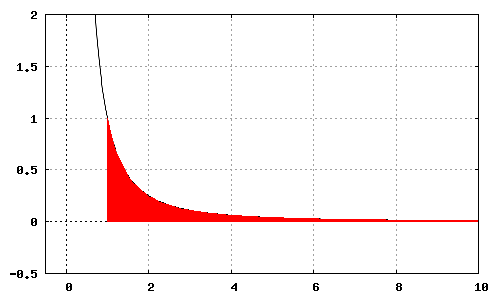
\includegraphics[width=3in]{example_1_4_1_1}

\end{exmp}

\line(1,0){60}
\linethickness{0.5mm}


\begin{exmp} Compute $\displaystyle \int_0^1 \frac{1}{\sqrt{x}}\ \mathrm{d}x$.\\
${}$\\

In this case, the integrand becomes infinite at the left limit of integration.  Formally, we are required to compute $\displaystyle \lim_{t \to 0^+} \displaystyle \int_t^1 \frac{1}{\sqrt{x}}\ \mathrm{d}x$:
${}$\\

\begin{verbatim}
(%i7) f(x):=1/sqrt(x)$
      limit(integrate(f(x),x,t,1),t,0);
      
"Is  "t-1"  positive, negative, or zero?"negative;
"Is  "t"  positive, negative, or zero?"positive;

(%o8) 2
\end{verbatim}

Repeating the calculation less formally:

\begin{verbatim}
(%i9) integrate(f(x),x)$
      F(x):=''(%);
(%o10) F(x):=2*sqrt(x)
(%i11) F(1)-F(0);
(%o11) 2
\end{verbatim}


Again, it is interesting to make a plot.  This time we have a shaded area that is infinitely high, yet finite.  We encounter an error when shading at a vertical asymptote, so the shading is set to start at $x=.001$ instead of $0$.

\begin{verbatim}
(%i12) wxdraw2d(
       grid=true,
       xaxis=true,
       yaxis=true,
       xrange=[-.5,1.5],
       yrange=[-.5,10],
       color=black,
        explicit(f(x),x,-.5,1.5),
       filled_func=true,
        filled_func=f(x),
        explicit(0,x,.001,1),
       filled_func=false
       );
\end{verbatim}


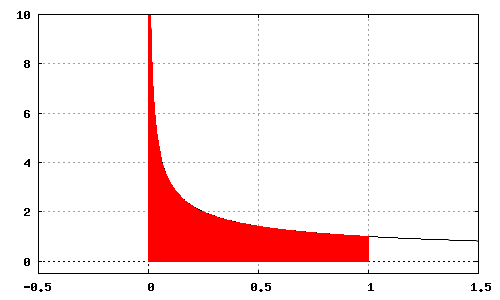
\includegraphics[width=3in]{example_1_4_2_1}

\end{exmp}

\line(1,0){60}
\linethickness{0.5mm}


\begin{exmp} Compute $\displaystyle \int_1^4 \frac{1}{(x-3)^2}\ \mathrm{d}x$.\\
${}$\\
${}$\\
This time, the integration interval contains a discontinuity.  To compute the integral formally, we have to break the it into two parts at the discontinuity, then phrase each piece as a limit:  $\displaystyle \int_1^4 \frac{1}{(x-3)^2}\ \mathrm{d}x = \displaystyle \lim_{t \to 3^-} \displaystyle \int_1^t \frac{1}{(x-3)^2}\ \mathrm{d}x + \displaystyle \lim_{t \to 3^+} \displaystyle \int_t^4 \frac{1}{(x-3)^2}\ \mathrm{d}x$\\

${}$\\
${}$\\
wxMaxima flags the area functions as divergent before we can compute the limits:

\begin{verbatim}
(%i13) f(x):=1/(x-3)^2$
(%i14) integrate(f(x),x,1,t);

"Is  "t-1"  positive, negative, or zero?"positive;
"Is  "t-2"  positive, negative, or zero?"positive;

defint: integral is divergent.
 -- an error. To debug this try: debugmode(true);
\end{verbatim}


This answer is unsatisfying, so we approach the problem by computing the antiderivative of $f(x)$:

\begin{verbatim}
(%i15) A:integrate(f(x),x);
(%o15) -1/(x-3)
\end{verbatim}

Now we compute the first integral using a limit on a difference of antiderviatives $\displaystyle \lim_{x \to 3^-} [A(x)-A(1)]$:

\begin{verbatim}
(%i16) limit(A,x,3,minus)-subst(1,x,A);
(%o16) infinity-1/2
\end{verbatim}

We see that $\displaystyle \lim_{t \to 3^-} \displaystyle \int_1^t \frac{1}{(x-3)^2}\ \mathrm{d}x=+\infty$.  The second integral also evaluates to $+\infty$ (the calculation is left as an Exercise).\\




${}$\\
One interesting point about this problem is that we can obtain the wrong answer if we don't consider the discontinutity:

\begin{verbatim}
(%i18) integrate(f(x),x)$
       F(x):=''(%);
(%o18) F(x):=-1/(x-3)
(%i19) F(4)-F(1);
(%o19) -3/2
\end{verbatim}

That's a good reminder to always check for problematic points on the interval of interest!\\
${}$\\


We finish with a quick plot for the sake of completeness:

\begin{verbatim}
(%i17) wxdraw2d(
       grid=true,
       xaxis=true,
       yaxis=true,
       xrange=[0,5],
       yrange=[-.5,25],
       color=black,
        explicit(f(x),x,0,5),
       filled_func=true,
        filled_func=f(x),
        explicit(0,x,1,4),
       filled_func=false
       );
\end{verbatim}

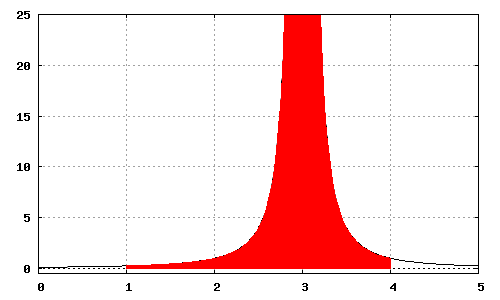
\includegraphics[width=3in]{example_1_4_3_1}






\end{exmp}

\line(1,0){60}
\linethickness{0.5mm}
\pagebreak

\section{Module 1 Exercises}\label{Module 1 Exercises}

\begin{enumerate}

\item  Use \verb|integrate| to find a decimal approximation for the definite integral $\displaystyle \int _4^7 \frac{1}{x^2\cdot \sqrt{x-3}}\ \mathrm{d}x$, then make a shaded plot with an appropriate scale to show the area represented by the integral.

\item  Repeat the first exercise by defining an area function $A(x)$ and evaluating $A(7)-A(4)$.  You are free to choose any ``starting point'' you like, as long as it doesn't create a divergent integral.

\item  Repeat the first exercise by computing the antiderivative, $F(x)$ for $f(x)=\displaystyle \frac{1}{x^2\cdot \sqrt{x-3}}$ and evaluating $F(x)|_4^7$.

\item Compute $\displaystyle \int x^2\cdot \sqrt{1-x^3}\ \mathrm{d} x$ by making a $u$-substitution in the style of Example 1.2.1.


\item Use a $u$-substitution to compute $\displaystyle \int_0^{\frac{\pi}{6}} \sin{(3x)} \cos^3{(3x)}\ \mathrm{d}x$ in the style of Example 1.2.2.  Finish the calculation by transforming the limits in terms of $u$ rather than transforming the antiderivative in terms of $x$.


\item Use \verb|trigreduce| to apply ``double angle formulas'' to the integrand of $\displaystyle \int \cos^4{x}\ \mathrm{d} x$.  Perform all the resulting integrals by inspection.  Check your final answer using \verb|diff| followed by \verb|trigexpand| and \verb|trigsimp|.

\item Compute the integral $\displaystyle \int_{-3}^{3} \sqrt{9-x^2}\ \mathrm{d}x$ by performing a trigonometric substitution in the style of Example 1.2.3.  Make a shaded plot with a square aspect ratio by using \verb|dimensions|.  Explain how this integral can be computed using a simple formula from geometry.

\item Define a function \verb|CTS(x,a,b,c)| to complete the square, given the coefficients in a quadratic polynomial in the form $ax^2+bx+c$.  Use your function to complete the square on $2x^2-3x+7$.  Check your answer using \verb|expand|.


\item Use \verb|CTS(x,a,b,c)| to complete the square in the denominator of $\displaystyle \int \frac{\mathrm{d}x}{9x^2+12x+10}$.  Make a $u$-substitution to obtain the form $\displaystyle \int \frac{1}{u^2+1}\ \mathrm{d}u$ (with possibly some constants in front).  Finally, perform the integral and transform your answer back to $x$.  Check using \verb|diff|.

\item Finish the integral in Example 1.3.3:  $\displaystyle \int \frac{5x-\frac{2}{3}}{3x^2+2x+2}\ \mathrm{d}x-\displaystyle \int \frac{5}{3(x+1)}\ \mathrm{d}x$.  The second integral can already be performed by inspection.  The first integral can be transformed into two integrals $\displaystyle \int \frac{\mathrm{d}u}{u} + \displaystyle \int \frac{\mathrm{constants}}{3x^2+2x+2}\ \mathrm{d}x$.  Finish the first piece by inspection, then use \verb|CTS(x,a,b,c)| to transform the denominator in the second piece.  Make the appropriate $u$-substitution to obtain an integral that can be done by inspection.  Finally, check your answer using \verb|diff|.

\item Integrate $\displaystyle \int x\cdot \sin^2{x}\ \mathrm{d}x$ using integration by parts in the style of Example 1.3.1.

\item When integration by parts is applied to a definite integral, we get $\displaystyle \int_a^b u\ \mathrm{d}v = uv|_a^b - \displaystyle \int_a^b v\ \mathrm{d}u$.  Apply this formula to compute $\displaystyle \int_0^2 x\cdot e^x \ \mathrm{d}x$. 


\item Compute $\displaystyle \int e^{-\alpha t} \cos{\beta t}\ \mathrm{d} t$ using integration by parts.  Set up an equation with $\displaystyle \int e^{-\alpha t} \cos{\beta t}\ \mathrm{d} t$ on the left-hand side and the results of your first parts decomposition on the right hand side.  Repeat for another application of integration by parts.  After two iterations of integration by parts,  you should recognize a term containing the original integral on the right hand side.  Combine the two terms containing the original integral on the left hand side, and solve for the value of this integral.  Check your answer using \verb|diff|. Throughout your calculations, use \verb|%alpha| and \verb|%beta|.  You will have to use \verb|declare| for \verb|diff| to recognize $\alpha$ and $\beta$ as constants.

\item Make a function \verb|DOS(x,a,b)| to factor $ax^2-b$ into two linear factors even if $a$ and $b$ are not  perfect squares.  Apply \verb|DOS(x,a,b)| to the denominator of $\displaystyle \int \frac{\mathrm{d}x}{2x^2-5}$.  Now perform a partial fractions decomposition in the style of Example 1.3.3 and finish the integral by inspection.

\item Compute the integral from the previous Exercise by using a trigonometric substitution in the style of Examples 1.2.3 and 1.2.4.  Verify that your answer is the same as before.

\item Compute the integral $\displaystyle \int \frac{1}{x\cdot \sqrt{1-x}}\ \mathrm{d}x$ starting with the $u$-substitution $u^2=1-x$.  Once the integral is transformed in terms of $u$, use \verb|partfrac| to perform a partial fractions decomposition, then finish the $u$ integrals by inspection.  Don't forget to transform your final answer back to $x$.

\item Compute the second improper integral from Example 1.4.3:  $\displaystyle \lim_{t \to 3^+} \displaystyle \int_t^4 \frac{1}{(x-3)^2}\ \mathrm{d}x$


\item Compute $\displaystyle \int_0^{\infty} \frac{1}{x^2+a^2}\ \mathrm{d}x$ by making an appropriate trigonometric substitution and transforming the limits of integration in terms of the substitution variable.



\end{enumerate}

\pagebreak

\chapter{Numerical Integration Techniques}

\vspace*{\fill}

\minitoc

\vspace*{\fill}


\flushleft{\textbf{\Large Key Commands Included in This Module}}
\newline
\newline

\begin{tabular}{l l l}
 \verb|integrate   |   &\verb|sum   |   &\verb|rhs   |   \\
 \verb|float   |   &\verb|for-do   |   &\verb|kill(all)   |   \\
 \verb|rectangle   |   &\verb|polygon   |   &\verb|ratprint   |   \\
 \verb|makelist   |   &\verb|sublis   |   &\verb|quad_qag   |   \\
 \verb|wxdraw2d   |   &\verb|solve   |   &\verb|random   |   \\
\end{tabular}



\pagebreak
\section{Midpoint Sums}\label{Midpoint Sums}

If the analytic formula for a function $f(x)$ is known, we can approximate $\displaystyle \int_a^b f(x)\ \mathrm{d}x$ by using a midpoint Riemann sum.  That is, we break the interval $[a,b]$ into $n$ sub-intervals at the cut-points $a=x_0,x_1,x_2,...,x_{n-1},x_n=b$, then we use the midpoint of each subinterval to compute the height of each rectangle in the approximation.\\
${}$\\
We choose sub-intervals of equal width $\Delta x = \frac{b-a}{n}$, and the height of the $i^{th}$ rectangle is given by $f\left( \frac{x_{i-1}+x_i}{2}\right)$.  Adding the rectangle areas, we obtain the midpoint approximation:

\[f\left( \frac{x_{0}+x_1}{2}\right) \Delta x + f\left( \frac{x_{1}+x_2}{2}\right) \Delta x + \dots + f\left( \frac{x_{n-1}+x_n}{2}\right) \Delta x = \sum_ {i=1}^{n} f\left( \frac{x_{i-1}+x_i}{2}\right) \Delta x\]

The midpoint approximation becomes more accurate as $n$ grows, and the rectangles become narrower.\\

\begin{exmp} Show that wxMaxima cannot compute $\displaystyle \int_0^3 e^{\sin{x}}\ \mathrm{d}x$ analytically.  Compute the $n=20$ midpoint sum approximating the integral, and make a plot illustrating the midpoint rectangles.\\
${}$\\

We start by defining $f(x)$ and attempting to use \verb|integrate|.  wxMaxima simply repeats the integral to us, indicating that it can't find an analytical solution.

\begin{verbatim}
(%i1) f(x)=%e^(sin(x))$
      integrate(f(x),x,0,3);
(%o2) integrate(%e^sin(x),x,0,3)
\end{verbatim}

Now we define $\Delta x$ and $x_i$ and compute the midpoint approximation:

\begin{verbatim}
(%i3) delx:(3-0)/20;
      x(i):=''delx*i;
(%o3) 3/20
(%o4) x(i):=3/20*i

(%i5) float(sum(f((x(i)+x(i-1))/2)*delx,i,1,20));
(%o5) 6.058676126838001
\end{verbatim}

We use \verb|rectangle| inside of \verb|makelist| to generate a list of rectangles that works inside \verb|wxdraw2d|.  Note that \verb|rectangle| draws a rectangle based on a list of just two vertices at opposite corners.\\

\begin{verbatim}
(%i6) RECTANGLES:makelist(rectangle([x(i-1),0],[x(i),f((x(i)+x(i-1))/2)])
      ,i,1,20)$
(%i7) load(draw)$
      wxdraw2d(
      grid=true,
      xaxis=true,
      yaxis=true,
      yrange=[-1,3.2],
      title="n=20 Midpoint Sum for f(x) on [0,3]",
      color=black,
      fill_color=red,
      border=true,
       RECTANGLES,
       explicit(f(x),x,-1,4)
      );
\end{verbatim}

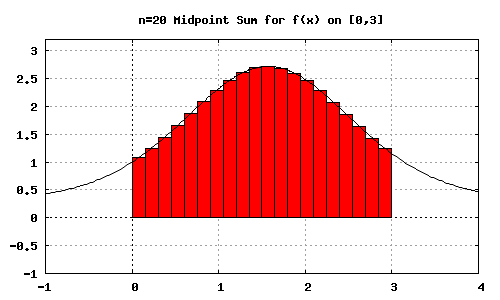
\includegraphics[width=3in]{example_2_1_1_1}

\end{exmp}

\line(1,0){60}
\linethickness{0.5mm}



\begin{exmp} Write a \verb|for-do| loop to compute midpoint approximations of $\displaystyle \int_0^3 e^{\sin{x}}\ \mathrm{d}x$ using $n=20,40,60,\dots $ until the approximation settles down to at least three decimal places.\\
${}$\\
First we adapt our $n=20$ sum to work more generally:

\begin{verbatim}
(%i8) f(x):=%e^(sin(x))$
      delx(n):=(3-0)/n$
      x(i,n):=''delx(n)*i$
(%i9) SUM(n):=sum((f((x(i-1,n)+x(i,n))/2)*delx(n)),i,1,n)$
\end{verbatim}

Now we write and execute the do-loop:

\begin{verbatim}
(%i10) (print("n....MIDPOINT SUM"),
        for k:1 thru 10 do
        (n:(20*k),
         S:(float(SUM(n))),
         print(n,"","","",S))
       );
       
 n....MIDPOINT SUM
20    6.058676126838001
40    6.057171126434241
60    6.056892460067756
80    6.05679492965105
100   6.056749787496514
120   6.056725265963955
140   6.056710480298045
160   6.05670088385024
180   6.056694304565428
200   6.056689598445805
\end{verbatim}

It looks like the integral is safely settled down to $6.056$, so 10 iterations is sufficient.


\end{exmp}

\line(1,0){60}
\linethickness{0.5mm}
\pagebreak



\pagebreak
\section{Trapezoid Sums}\label{Trapezoid Sums}
\subsection{For a Function Defined Analytically}

When the analytic formula for $f(x)$ is known, we can approximate $\displaystyle \int_a^b f(x)\ \mathrm{d}x$ by using narrow trapezoids, each with a height of $f(x_{i-1})$ on the left side, and $f(x_i)$ on the right side.  Once again, we divide the interval $[a,b]$ into $n$ equal sub-intervals of width $\Delta x = \frac{b-a}{n}$, and the area of each trapezoid is given by $\frac{\left(f(x_{i-1})+f(x_i)\right)}{2}\cdot \Delta x$.  The area approximation is then given by:

\[\frac{\left(f(x_{0})+f(x_1)\right)}{2}\cdot \Delta x+
\dots +
\frac{\left(f(x_{n-1})+f(x_n)\right)}{2}\cdot \Delta x=
\sum_{i=1}^{n} \frac{\left(f(x_{i-1})+f(x_i)\right)}{2}\cdot \Delta x\]

\begin{exmp} Compute the $n=20$ trapezoid approximation for $\displaystyle \int_0^3 e^{\sin{x}}\ \mathrm{d}x$, and compare the answer to the midpoint approximations performed in the last example.  Make a plot to illustrate the approximation.\\
${}$\\

We begin by defining $\Delta x$, $x_i$ and the area of a single trapezoid, then we compute the sum:

\begin{verbatim}
(%i1) f(x):=%e^(sin(x))$
      delx:(3-0)/20$
      x(i):=delx*i$
      AREA(i):=((f(x(i-1))+f(x(i)))/2)*delx;
(%o4) AREA(i):=(f(x(i-1))+f(x(i)))/2*delx
(%i5) float(sum(AREA(i),i,1,20));
(%o5) 6.052656613881449
\end{verbatim}

When we compare this approximation to the $n=20$ midpoint sum, we see that the trapezoid approximation is actually worse than the midpoint approximation in this case.  The trapezoids systematically \textit{underestimate} the area because $f(x)$ is concave down on almost the entire interval of interest.  \\

${}$\\
Once again, we use \verb|makelist| to plot the trapezoid approximation.  This time we have to use \verb|polygon|, which expects a list of vertices in order around each trapezoid:\\

\begin{verbatim}
(%i6) TRAPEZOIDS:makelist(polygon([ [x(i-1),0], [x(i),0], 
           [x(i),f(x(i))], [x(i-1),f(x(i-1))] ]),i,1,20)$
(%i7) wxdraw2d(
      grid=true,
      xaxis=true,
      yaxis=true,
      yrange=[-1,3.2],
      color=black,
      border=true,
      fill_color=red,
       TRAPEZOIDS,
       explicit(f(x),x,-1,4)
      );
\end{verbatim}


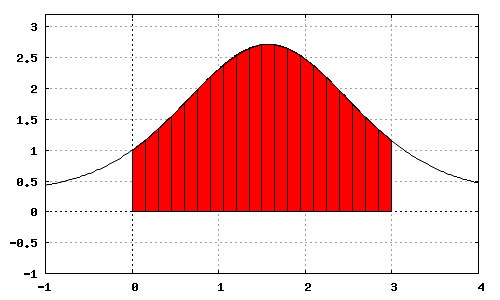
\includegraphics[width=3in]{example_2_2_1_1}



\end{exmp}

\line(1,0){60}
\linethickness{0.5mm}


\subsection{For a Discrete Data Set}

If the analytic formula for $f(x)$ is \textit{not} known (as in a list of data points), we can still make a trapezoid approximation by simply ``connecting the dots'' between the points we are given.  \\
${}$\\
\begin{exmp} In a physics experiment, the velocity of an object is measured every $0.01 \mathrm{s}$ to obtain the following data set:


\begin{verbatim}
     t(s).....v(m/s)
 
     0.01     2.3
     0.02     1.8
     0.03     1.8
     0.04     1.7
     0.05     1.5
     0.06     1.5
     0.07     1.3
     0.08     1.1
     0.09     0.8
     0.10     0.5
\end{verbatim}

Compute the total displacement of the object $\Delta x = \displaystyle \int_{.01}^{.10} v(t)\ \mathrm{d}t$, by using a trapezoid approximation, then make a plot of $v(t)$ to illustrate the approximation.\\
${}$\\
In this example, the data set is equally spaced on the $t$-axis, allowing us to define a fixed $\Delta t = 0.01$.  We enter the data in list format starting with lists of the $x$ coordinates and $y$ coordinates, use \verb|makelist| to create ordered pairs and compute the sum of trapezoid areas by calling the necessary list elements:

\begin{verbatim}
(%i1) X:[.01,.02,.03,.04,.05,.06,.07,.08,.09,.10]$
      Y:[2.3,1.8,1.8,1.7,1.5,1.5,1.3,1.1,.8,.5]$
      POINTS:makelist([X[i],Y[i]],i,1,10)$
      delt:0.01$
(%i5) TRAPEZOID(i):=0.5*(Y[i]+Y[i+1])*delt$
      sum(TRAPEZOID(i),i,1,9);
(%o6) 0.129
\end{verbatim}

We obtain an approximate displacement of $\Delta x \approx 0.129 \mathrm{m}$.  Now we proceed with the plot by defining a list of trapezoids and calling our list elements:

\begin{verbatim}
(%i7) TRAPEZOIDS:makelist(polygon([[X[i],0],
       [X[i+1],0],[X[i+1],Y[i+1]],[X[i],Y[i]]]),i,1,9)$
(%i8) wxdraw2d(
      grid=true,
      xaxis=true,
      yaxis=true,
      xrange=[0,.11],
      yrange=[0,2.5],
      title="Velocity-Time Data",
      color=black,
      border=true,
      fill_color=red,
       TRAPEZOIDS,
      point_type=7,
       points(POINTS)
      );
\end{verbatim}

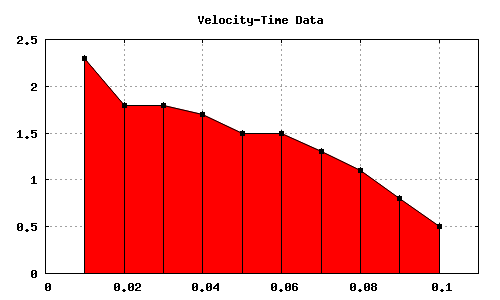
\includegraphics[width=3in]{example_2_2_2_1}

\end{exmp}

\line(1,0){60}
\linethickness{0.5mm}
${}$\\
\begin{exmp} The force exerted by a spring is measured as a function of stretch length to yield the following data set:\\

\begin{verbatim}
     x(m).....F(N)
     0.10     10
     0.15     20
     0.19     30
     0.22     40
     0.25     50
     0.28     60
     0.30     70
     0.32     80
     0.33     90
     0.34    100
\end{verbatim}

Use a trapezoid approximation to compute the work done on the spring:  $W=\displaystyle \int_{.10}^{.34} F(x)\ \mathrm{d}x$.  Make a plot of $F(x)$ to illustrate the trapezoid approximation.\\
${}$\\
${}$\\
This time the spacing is uneven on the $x$-axis, so we can't define a fixed trapezoid width.  We adjust our trapezoid areas to use differences of adjacent $x$ values for the width.

\begin{verbatim}
(%i9) kill(all)$
      X:[.1,.15,.19,.22,.25,.28,.30,.32,.33,.34]$
      Y:[10,20,30,40,50,60,70,80,90,100]$
      POINTS:makelist([X[i],Y[i]],i,1,10)$
(%i4) TRAPEZOID(i):=0.5*(Y[i]+Y[i+1])*(X[i+1]-X[i])$
      sum(TRAPEZOID(i),i,1,9);
(%o5) 10.4
\end{verbatim} 

We see that the total work on the spring is $W \approx 10.4\ \mathrm{J}$.  We plot the approximation as before:\\

\begin{verbatim}
(%i6) TRAPEZOIDS:makelist(polygon([ [X[i],0],[X[i+1],0],
      [X[i+1],Y[i+1]],[X[i],Y[i]] ]),i,1,9)$
(%i7) wxdraw2d(
      grid=true,
      xaxis=true,
      yaxis=true,
      xrange=[0,.4],
      yrange=[0,110],
      title="Force-Displacement Data",
      color=black,
      border=true,
      fill_color=red,
       TRAPEZOIDS,
      point_type=7,
       points(POINTS)
      );
\end{verbatim}


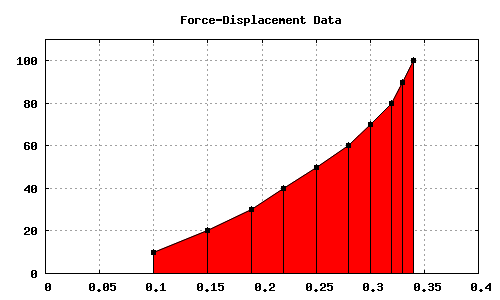
\includegraphics[width=3in]{example_2_2_3_1}

\end{exmp}

\line(1,0){60}
\linethickness{0.5mm}
\pagebreak

\pagebreak
\section{Simpson's Method}\label{Simpson's Method}
\subsection{For a Function Defined Analytically}

The midpoint and trapezoid approximations are both examples of approximations by \textit{interpolating polynomials}.  The midpoint approximation uses polynomials of degree 0 (constant functions) to estimate the area on each sub-interval, and the trapezoid approximation uses polynomials of degree 1 (lines) to estimate the area on each sub-interval.  Simpson's method simply extends the idea to polynomials of degree 2; i.e., we approximate the function with a sequence of \textit{parabolas} on each pair of subintervals.\\
${}$\\

Each Simpson's Method parabola passes through three consecutive points on the function we wish to integrate.  It is always possible to compute the formula for a parabola passing through three points, because the formula for a parabola $y=ax^2+bx+c$ has three undetermined coefficients.  The points define a system of three equations and three unknowns.

\begin{exmp} Compute a formula for the parabola passing through $(-1,1)$, $(0,3)$ and $(2,-1)$, then make a plot of the parabola together with the given points.\\

${}$\\

We start by defining a general equation for the parabola, $y=ax^2+bx+c$, then we use the points to define a system of equations.  After solving the system, we substitute $a,b,c$ back into the general equation:

\begin{verbatim}
(%i1) EQN:y=a*x^2+b*x+c$
      EQN1:sublis([x=-1,y=1],EQN);
      EQN2:sublis([x=0,y=3],EQN);
      EQN3:sublis([x=2,y=-1],EQN);
      
(%o2) 1=c-b+a
(%o3) 3=c
(%o4) -1=c+2*b+4*a

(%i5) solve([EQN1,EQN2,EQN3],[a,b,c]);
(%o5) [[a=-4/3,b=2/3,c=3]]
(%i6) sublis([a=-4/3,b=2/3,c=3],EQN);

(%o6) y=-(4*x^2)/3+(2*x)/3+3
\end{verbatim}

Finally, we produce a plot of the parabola passing through $(-1,1)$, $(0,3)$ and $(2,-1)$:

\begin{verbatim}
(%i7) PARABOLA:rhs(%);
(%o7) -(4*x^2)/3+(2*x)/3+3
(%i8) wxdraw2d(
       grid=true,
       xaxis=true,
       yaxis=true,
       xrange=[-3,3],
       yrange=[-2,4],
       title="Parabola passing through [-1,1], [0,3] and [2,-1]",
       color=black,
        explicit(PARABOLA,x,-3,3),
       color=red,
       point_type=7,
        points([ [-1,1],[0,3],[2,-1] ])
       );
\end{verbatim}

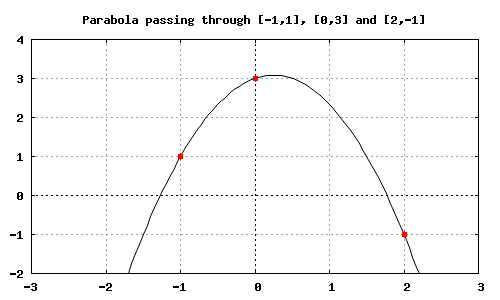
\includegraphics[width=3in]{example_2_3_1_1}
\end{exmp}
\line(1,0){60}
\linethickness{0.5mm}

${}$\\

We apply Simpson's Method by approximating $f(x)$ with a separate parabola for each pair of consecutive sub-intervals.  The area under each parabola is easily computed, then we sum all the areas to obtain the approximation to $\displaystyle \int_{a}^{b} f(x)\ \mathrm{d}x$.  If the number of sub-intervals, $n$, is even and the sub-intervals have equal width, the result simplifies to \textit{Simpson's Formula}, which can be found in any calculus text.

\begin{exmp} Find a Simpson's Method approximation for $\displaystyle \int_0^3 e^{\sin{x}}\ \mathrm{d}x$ using $n=6$.  Make a plot showing $e^{\sin{x}}$ together with a relevant section of each interpolating parabola.\\
${}$\\
Simpson's Method tells us to fit a parabola to each consecutive \textit{pair} of sub-intervals, so we only need three parabolas for this example:\\
${}$\\
\verb|     PARABOLA1| connects $(x_0,f(x_0))$, $(x_1,f(x_1))$ and $(x_2,f(x_2))$\\
\verb|     PARABOLA2| connects $(x_2,f(x_2))$, $(x_3,f(x_3))$ and $(x_4,f(x_4))$\\
\verb|     PARABOLA3| connects $(x_4,f(x_4))$, $(x_5,f(x_5))$ and $(x_6,f(x_6))$\\
${}$\\
For large values of $n$, we can fully automate the process of finding the parabolas.  Here we take a hybrid approach by automating only the computation of \verb|EQN(i)| generated by substituting $(x_i,f(x_i))$ into the general equation of a parabola:

\begin{verbatim}
(%i9) f(x):=%e^(sin(x))$
(%i10) GENEQN:Y=a*X^2+b*X+c$
(%i11) delx:0.5$
(%i12) x(i):=i*delx$
(%i13) EQN(i):=(sublis([X=x(i),Y=f(x(i))],GENEQN))$
\end{verbatim}

Now we have three systems of equations to solve and three parabolas to construct.  Note that the substitution of $a$, $b$, and $c$ back into \verb|GENEQN| requires an extra \verb|[1]| to call the bracketed coefficients from the output of \verb|solve|:

\begin{verbatim}
(%i14) COEFFS1:float(solve([EQN(0),EQN(1),EQN(2)],[a,b,c]));
(%o14) [[a=0.17896846366337,b=1.140808361052482,c=1.0]]
(%i15) PARABOLA1:rhs(sublis(COEFFS1[1],GENEQN));
(%o15) 0.17896846366337*X^2+1.140808361052482*X+1.0

(%i16) COEFFS2:float(solve([EQN(2),EQN(3),EQN(4)],[a,b,c]));
(%o16) [[a=-1.241214965266928,b=3.886445799099931,c=-0.32545400911715]]
(%i17) PARABOLA2:rhs(sublis(COEFFS2[1],GENEQN));
(%o17) -1.241214965266928*X^2+3.886445799099931*X-0.32545400911715

(%i18) COEFFS3:float(solve([EQN(4),EQN(5),EQN(6)],[a,b,c]));
(%o18) [[a=-0.0090668352651675,b=-1.285680715174632,c=5.090206499424927]]
(%i19) PARABOLA3:rhs(sublis(COEFFS3[1],GENEQN));
(%o19) -0.0090668352651675*X^2-1.285680715174632*X+5.090206499424927
\end{verbatim}

Now that we have the equations of all three parabolas, we can integrate each one on the relevant sub-intervals $(x_0,x_2)$, $(x_2,x_4)$, and $(x_4,x_6)$:

\begin{verbatim}
(%i20)  float(integrate(PARABOLA1,X,x(0),x(2))
              +integrate(PARABOLA2,X,x(2),x(4))
              +integrate(PARABOLA3,X,x(4),x(6))
             );
(%o20) 6.056688193799587
\end{verbatim}

Finally, we plot $f(x)$ together with the interpolating parabolas.  Each parabola is plotted slightly outside the actually integrated range just to make it easier to see what's going on:

\begin{verbatim}
(%i21) wxdraw2d(
       grid=true,
       xaxis=true,
       yaxis=true,
       xrange=[-1,4],
       yrange=[-1,3.2],
       title="f(x) together with three interpolating parabolas",
       color=black,
       line_width=2,
        explicit(f(x),x,0,3),
       line_type=dots,
       color=red,
       line_width=1,
       key="PARABOLA1",
        explicit(PARABOLA1,X,x(0)-.4,x(2)+.4),
       color=dark_green,
       key="PARABOLA2",
        explicit(PARABOLA2,X,x(2)-.4,x(4)+.4),
       color=blue,
       key="PARABOLA3",
        explicit(PARABOLA3,X,x(4)-.4,x(6)+.4)
       );
\end{verbatim}


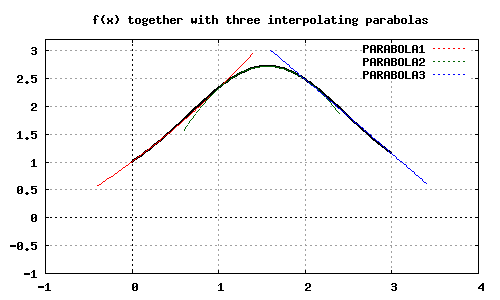
\includegraphics[width=3in]{example_2_3_2_1}

\end{exmp}

\line(1,0){60}
\linethickness{0.5mm}


\subsection{*For a Discrete Data Set}

Simpson's Method can still be used to approximate an integral if $n$ is odd or the sub-interval spacing varies.  Thus, we can apply the method to realistic data sets.  We must be particularly careful if $n$ is odd, as the integration interval cannot be neatly split into pairs of sub-intervals -- in this case we can just use the trapezoid approximation on the last sub-interval.

\begin{exmp} 
For the same data set as Example 2.2.3, compute the total work done on the spring $W=\displaystyle \int_{.10}^{.34} F(x)\ \mathrm{d}x$ by using interpolating parabolas on the first 8 sub-intervals and a trapezoid on the last interval.  Make a plot illustrating the approximation.

\begin{verbatim}
     x(m).....F(N)
     0.10     10
     0.15     20
     0.19     30
     0.22     40
     0.25     50
     0.28     60
     0.30     70
     0.32     80
     0.33     90
     0.34    100
\end{verbatim}

This time, we have to work with a list of specific data points rather than a formula for the function we wish to integrate.  In addition, we make the effort to automate as much as we possibly can by using \verb|makelist|.  We also hide many intermediate results for the sake of brevity.  We begin by defining and solving the system of equations for each interpolating parabola.  The indices \verb|2*k+1|, \verb|2*k+2| and \verb|2*k+3| are used to call points $\lbrace (x_1,y_1),(x_2,y_2),(x_3,y_3) \rbrace$, $\lbrace (x_3,y_3),(x_4,y_4),(x_5,y_5) \rbrace$, $\lbrace (x_5,y_5),(x_6,y_6),(x_7,y_7) \rbrace$, $\lbrace (x_7,y_7),(x_8,y_8),(x_9,y_9) \rbrace$ for the four parabolas:


\begin{verbatim}
(%i22) kill(all)$
(%i1) x:[.1,.15,.19,.22,.25,.28,.30,.32,.33,.34]$
      y:[10,20,30,40,50,60,70,80,90,100]$
      POINTS:makelist([x[i],y[i]],i,1,10)$
(%i4) GENEQN:Y=a*X^2+b*X+c$
(%i5) EQN(i):=(sublis([X=x[i],Y=y[i]],GENEQN))$
(%i6) ratprint:false$
(%i7)  SOLUTIONS:makelist(float(solve([EQN(2*k+1),EQN(2*k+2),EQN(2*k+3)],
                               [a,b,c])),k,0,3);
(%o7) [[[a=555.5555555555555,b=61.11111111111111,c=-1.666666666666667]],
      [[a=0.0,b=333.3333333333333,c=-33.33333333333334]],
      [[a=3333.333333333334,b=-1433.333333333333,c=200.0]],
      [[a=16666.66666666667,b=-9833.333333333334,c=1520.0]]]
\end{verbatim}

Next, we substitute each of these solutions for $a,b,c$ into the general equation $y=ax^2+bx+c$ to get an equation for each interpolating parabola.  The trickiest part of this step is recognizing the list format of \verb|SOLUTIONS| -- it is a list of solutions, but each solution is represented as a list containing one element (the comma-delimited solutions).  We call each element using \verb|SOLUTIONS[l+1]|, then we extract each solution by using an additional \verb|[1]|.  A list of integrals is then computed, each on the appropriate sub-interval.  Finally, the integrals are summed:

\begin{verbatim}
(%i8) intPARABOLAS:makelist(rhs(sublis((SOLUTIONS[l+1])[1],GENEQN)),l,0,3)$
(%i9) INTEGRALS:makelist(integrate(intPARABOLAS[m+1],X,x[2*m+1],
                   x[2*m+3]),m,0,3)$
(%i10) SIMPSONPART:float(sum(INTEGRALS[i],i,1,4));
(%o10) 9.388055555555557
\end{verbatim}

Now we add in the trapezoid defined on $(x_{9},x_{10})$ and compute the total area:

\begin{verbatim}
(%i11) TRAPEZOIDAREA:0.5*(y[10]+y[9])*(x[10]-x[9]);
(%o11) 0.95

(%i12) SIMPSONPART+TRAPEZOIDAREA;
(%o12) 10.33805555555556
\end{verbatim}

We see that the work integral comes out to $W\approx 10.34$, in close agreement to the trapezoid approximation ($W\approx 10.4$) we performed in Example 2.2.3.  \\
${}$\\
We finish by producing a plot of the Simpson's method approximation together with the trapezoid in the last sub-interval.  We use \verb|makelist| to prepare our parabolas to work in \verb|wxdraw2d|, including extending the domain slightly outside each interpolation interval to make the parabolas more visible.

\begin{verbatim}
(%i13) graphPARABOLAS:makelist(explicit(rhs(sublis((SOLUTIONS[l+1])[1],
       GENEQN)),X,x[2*l+1]-.01,x[2*l+3]+.01),l,0,3)$
(%i14) wxdraw2d(
       grid=true,
       xaxis=true,
       yaxis=true,
       xrange=[0,.4],
       yrange=[0,110],
       title="Data set with interpolating parabolas and one trapezoid",
       color=black,
       point_type=7,
       points(POINTS),
       color=red,
       line_type=dots,
        graphPARABOLAS,
       points_joined=true,
       color=black,
       line_type=solid,
        points([[x[9],y[9]],[x[10],y[10]]])
       );
\end{verbatim}

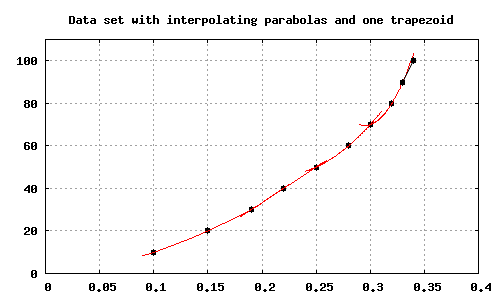
\includegraphics[width=3in]{example_2_3_3_1}

\end{exmp}

\line(1,0){60}
\linethickness{0.5mm}
\pagebreak

\pagebreak
\section{wxMaxima's Built-In Quadrature Methods}\label{wxMaxima's Built-In Quadrature Methods}

The term \textit{quadrature} is used to describe a variety of numerical integration methods.  We aren't interested in getting any deeper into numerical integration, and we will only use one numerical integration command, \verb|quad_qag|.  The syntax for \verb|quad_qag| is the same as the syntax for \verb|integrate|, except we must enter a fifth argument: an integer between 1 and 6 indicating the particular quadrature method.  The output of \verb|quad-qag| lists four numbers:  the first is the numerical approximation for the integral, the second is an approximation of the error (we ignore the others).\\
${}$\\

\begin{exmp} Compute the integral $\displaystyle \int_0^3 e^{\sin{x}}\ \mathrm{d}x$ using wxMaxima's built-in quadrature.  Compare the results of all 6 varieties of \verb|quad_qag|.

\begin{verbatim}
(%i1) f(x):=%e^(sin(x));
(%o1) f(x):=%e^sin(x)

(%i2) quad_qag(f(x),x,0,3,1);
(%o2) [6.05666953555315,5.7821357200595372*10^-12,45,0]
(%i3) quad_qag(f(x),x,0,3,2);
(%o3) [6.056669535553152,9.9580925827612082*10^-11,21,0]
(%i4) quad_qag(f(x),x,0,3,3);
(%o4) [6.05666953555315,6.7242539709168614*10^-14,31,0]
(%i5) quad_qag(f(x),x,0,3,4);
(%o5) [6.056669535553152,6.724253970916864*10^-14,41,0]
(%i6) quad_qag(f(x),x,0,3,5);
(%o6) [6.056669535553151,6.7242539709168627*10^-14,51,0]
(%i7) quad_qag(f(x),x,0,3,6);
(%o7) [6.056669535553151,6.7242539709168627*10^-14,61,0]
\end{verbatim}

We see that $\displaystyle \int_0^3 e^{\sin{x}}\ \mathrm{d}x\approx 6.057$, in close agreement with our previous approximations.  All methods from \verb|quad_qag| agree to many decimal places.


\end{exmp}

\line(1,0){60}
\linethickness{0.5mm}
\pagebreak


\section{A Monte Carlo Method}\label{A Monte Carlo Method}

The term \textit{Monte Carlo} is used to describe a variety of numerical methods that exploit random data.  We can formulate a simple Monte Carlo method to compute $\displaystyle \int_a^b f(x)\ \mathrm{d}x$ by equating two methods for computing the \textit{average value} of a function:\\

\begin{enumerate}

\item $f_{avg}=\displaystyle \frac{1}{b-a} \int_a^b f(x)\ \mathrm{d}x$
\item $f_{avg}\approx \displaystyle \frac{1}{N} \sum_{i=1}^N\ f(x_i)$ where $N$ values of $x_i$ are randomly generated on $[a,b]$.

\end{enumerate}

We equate the two calculations of $f_{avg}$ to obtain:
\[\int_a^b f(x)\ \mathrm{d}x \approx \frac{(b-a)}{N}\cdot \sum_{i=1}^N\ f(x_i)\]\\

In wxMaxima, we can generate random decimals on $[0,c]$ by entering \verb|random(c)|, making sure to express $c$ with a decimal place (if $c$ is expressed as an integer, \verb|random| only generates integers).

\begin{exmp} Compute $\displaystyle \int_0^3 e^{\sin{x}}\ \mathrm{d}x$ by using a Monte Carlo method with $N=1000$.  Repeat the calculation several times to get a sense for the uncertainty in the approximation.

\begin{verbatim}
(%i1) f(x):=%e^(sin(x))$

(%i2) ((3-0)/1000)*sum(f(random(3.0)),i,1,1000);
(%o2) 6.095597917343273

(%i3) ((3-0)/1000)*sum(f(random(3.0)),i,1,1000);
(%o3) 6.105455491341729

(%i4) ((3-0)/1000)*sum(f(random(3.0)),i,1,1000);
(%o4) 6.014387493961544
\end{verbatim}

In principle, we could perform a statistical analysis on several iterations of this method and use the standard deviation to quantify the uncertainty.  Perhaps it's better to push our computer harder by using $N=1,000,000$:

\begin{verbatim}
(%i5) ((3-0)/1000000)*sum(f(random(3.0)),i,1,1000000);
(%o5) 6.057168102573812
\end{verbatim}

This is very close to the answer we computed using \verb|quad_qag|.  My computer took close to two minutes to compute the approximation!

\end{exmp}

\line(1,0){60}
\linethickness{0.5mm}

\begin{exmp} Use a Monte Carlo method with $N=1000$ to compute $\displaystyle \int_2^3 e^{-x^2}\ \mathrm{d}x$.  Compare to the answer obtained by \verb|quad_qag|.\\
${}$\\
In order to use \verb|random| to generate random numbers on $[2,3]$, we start at $x=2$ and add random numbers between 0 and 1.0:

\begin{verbatim}
(%i6) f(x):=%e^(-x^2)$
(%i7) ((3-2)/1000)*sum(f(2+random(1.0)),i,1,1000);
(%o7) 0.0041199267231285
(%i8) quad_qag(%e^(-x^2),x,2,3,1);
(%o8) [0.0041259574970996,4.5908457058908545*10^-16,15,0]
\end{verbatim}

The Monte Carlo method was accurate to a few significant digits after sampling only 1000 random points.


\end{exmp}
\line(1,0){60}
\linethickness{0.5mm}
\pagebreak


\section{Module 2 Exercises}\label{Module 2 Exercises}

\begin{enumerate}

\item Compute $\displaystyle \int_1^e \cos{(\ln{x})}\ \mathrm{d}x$ using a midpoint approximation with $n=100$.  Make a plot illustrating the approximation in the style of Example 2.1.1.  Check your answer using \verb|integrate|.

\item  Repeat the previous Exercise using a trapezoid approximation in the style of Example 2.2.1.

\item  For $f(x)=\cosh{x}$ and $g(x)=\cos{x}$, compute the trapezoid approximations with $n=3$ on $[0,1]$, including plots illustrating the trapezoids.  Which approximation is an underestimate?  Which is an overestimate?  How are the errors linked to the concavity of $f$ and $g$?

\item  Voltage measurements are taken for one period in an AC circuit:

\begin{verbatim}
t(s)......v(t)(V)
0/1200     4.2
1/1200    67.5
2/1200   114.0
3/1200   112.7
4/1200    68.1
5/1200    -0.8
6/1200   -69.4
7/1200  -110.7
8/1200   114.1
9/1200   -68.7
10/1200   -4.6
\end{verbatim}

Compute $\displaystyle \int_0^{\frac{10}{1200}} v^2{(t)}\ \mathrm{d}t$ using a trapezoid approximation. Include a plot to illustrate the approximation.

\item  Repeat the previous Exercise using a Simpson's method approximation.  Include a plot showing the interpolating parabolas in the style of Example 2.3.3.

\item  Compute $\displaystyle \int_0^{\frac{\pi}{2}} \cos{(\sin{x})}\ \mathrm{d}x$ using \verb|quad_qag|.  Produce a shaded plot illustrating the area represented by the integral.

\item Repeat the integral from the previous Exercise using Simpson's method with $n=10$ in the style of Example 2.3.2.  Include a plot to illutrate the approximation.

\item  Repeat the integral from the previous Exercise using a Monte Carlo method with 1000 random points.
\pagebreak

\item  * We can use a Monte Carlo method to approximate $\pi$.  To visualize the method, start by using \verb|makelist| to generate 100 random points in a square of side-length 2 centered at the origin.  Plot the points together with the unit circle. Your plot should look something like this:\\

${}$\\
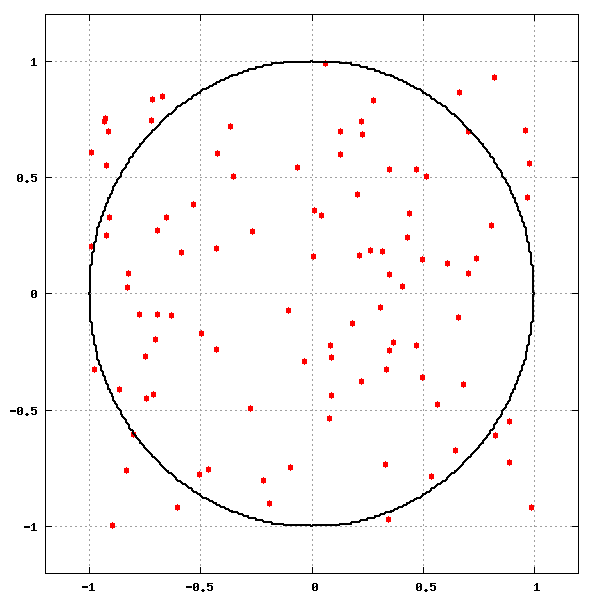
\includegraphics[width=2.5in]{example_2_e_x_1}

The area of the circle is given by $A_{circle}=\pi\cdot r^2=\pi$ and the area of the square is $A_{square}=4$, so we expect the fraction of points landing inside the circle is $\frac{A_{circle}}{A_{square}}=\frac{\pi}{4}$.  Use your plot to find an approximation to $\pi$.  

\item ** For the Monte Carlo method in the last example, we want to automate the process of counting the points that land inside the unit circle.  This can be accomplished using a \verb|for-do| loop to generate one point at a time and an \verb|if-then| statement to test whether or not each point is inside the circle.  Before the loop runs, we need to set the starting point for a counter \verb|n:0|.  If a point is inside the circle, we add 1 to the counter by writing \verb|n:n+1|. If we include any points landing right on the edge of the circle, the proper \verb|if-then| statement is:
\verb|  if (x^2+y^2<1 or x^2+y^2=1) then n:n+1|.\\
Finally, we use another \verb|if-then| statement telling wxMaxima to report the value of \verb|n| after the last iteration of the loop.\\
${}$\\
Construct the proper do-loop, starting with a small number of iterations until everything works properly.  As you are experimenting with the program, it is wise to ask wxMaxima to print \verb|n| at each iteration to make it easier to detect any problems in the calculation.  Once you are sure it's working, use the loop to generate 10,000 random points.  Use the fraction of points inside the circle to approximate $\pi$ three separate times to get a sense for the uncertainty in the answer.




\end{enumerate}

\pagebreak

\chapter{Geometric Applications of Integration}

\vspace*{\fill}

\minitoc

\vspace*{\fill}


\flushleft{\textbf{\Large Key Commands Included in This Module}}
\newline
\newline

\begin{tabular}{l l l}
 \verb|rectangle   |   &\verb|solve   |   &\verb|kill(all)   |   \\
 \verb|integrate   |   &\verb|find_root   |   &\verb|diff   |   \\
 \verb|ratprint:false   |   &\verb|wxdraw3d   |   &\verb|quad_qag   |   \\
 \verb|float   |   &\verb|parametric_surface   |   &\verb|   |   \\
 \verb|filled_func   |   &\verb|makelist   |   &\verb|   |   \\
\end{tabular}



\pagebreak
\section{Area Integrals}\label{Area Integrals}

\subsection{Area and Physical Integration}

Recall that $\displaystyle \int_{a}^{b} f(x) \ \mathrm{d}x$ gives us the area bounded between $f(x)$ and the $x$-axis.  It is useful to visualize an area \textit{element} at $x$ represented by a thin rectangle of width $\mathrm{d}x$.  We refer to this thin slice as $\mathrm{d}A$.  \\
${}$\\

\begin{center}
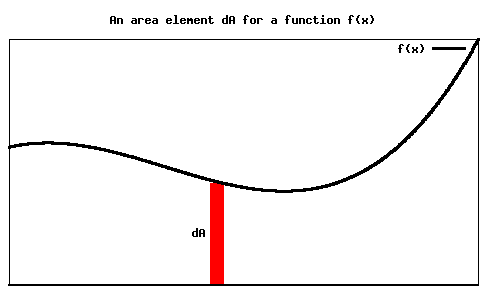
\includegraphics[width=3in]{figure_3_1_1_1}
\end{center}

Once  $\mathrm{d}A$ is phrased entirely in terms of one variable (here, $\mathrm{d}A=f(x)\cdot \mathrm{d}x$), we use integration to sum up all the area elements.  We can say $A=\displaystyle \int \mathrm{d}A = \displaystyle \int_{a}^{b} f(x) \ \mathrm{d}x$, and we view the integral as a \textit{summation device} to add up the $\mathrm{d}A$'s.  This conceptual approach is often called ``physical integration'', and it is very powerful when we apply integration in a geometric setting.\\
${}$\\

\begin{exmp}  Plot $f(x)=e^{-0.2\cdot x}\cdot \cos{x}$ on $[0,\frac{\pi}{2}]$ together with an area element at $x=1$.  Set up the integral $A= \displaystyle \int \mathrm{d}A$ and write $\mathrm{d} A$ in terms of $x$ to obtain a definite integral.  Finally, use wxMaxima to compute the area and make a shaded plot.\\
${}$\\

We start with the sketch of $f(x)$ and $dA$:

\begin{verbatim}
(%i1) f(x):=%e^(-0.2*x)*cos(x)$
      wxdraw2d(
      grid=true,
      xaxis=true,
      yaxis=true,
      title="f(x) with dA near x=1",
      color=black,
       explicit(f(x),x,0,%pi/2),
      border=false,
      color=red,
       rectangle([1,0],[1.05,f(1.05)]),
      color=black,
       label(["dA",0.95,0.2])
      );
\end{verbatim}

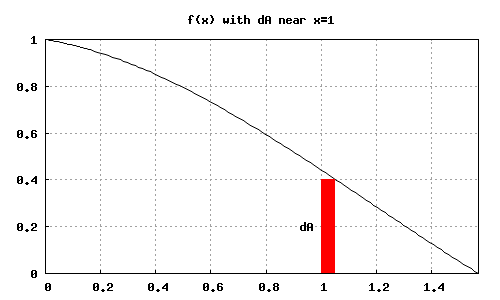
\includegraphics[width=3in]{example_3_1_1_1}
${}$\\
${}$\\
$\mathrm{d}A$ is just the product of height and width for the area element:  $f(x)\cdot \mathrm{d}x$.  Now we set up the integral:  $A = \displaystyle \int \mathrm{d}A = \displaystyle \int f(x)\ \mathrm{d}x = \displaystyle \int_0^{\frac{\pi}{2}} e^{-0.2\cdot x}\cdot \cos{x}\ \mathrm{d}x$\\
${}$\\
The integral is simple to compute using \verb|integrate|.  We start with \verb|ratprint:false| to suppress a list of \verb|ratprint| warnings, and we find a decimal approximation using \verb|float|:

\begin{verbatim}
(%i2) ratprint:false$
(%i3) integrate(f(x),x,0,%pi/2);
(%o3) (25*%e^(-%pi/10))/26+5/26
(%i4) float(%);
(%o4) 0.89461797216216
\end{verbatim}


We finish with a shaded plot:


\begin{verbatim}
(%i5) wxdraw2d(
      grid=true,
      xrange=[-0.5,2],
      yrange=[-0.5,1.2],
      xaxis=true,
      yaxis=true,
      title="Area Bounded by f(x) on [0,pi/2]",
      fill_color=grey,
      filled_func=true,
       filled_func=f(x),
       explicit(0,x,0,%pi/2),
      filled_func=false,
      color=black,
       explicit(f(x),x,-0.5,2)
      );
\end{verbatim}

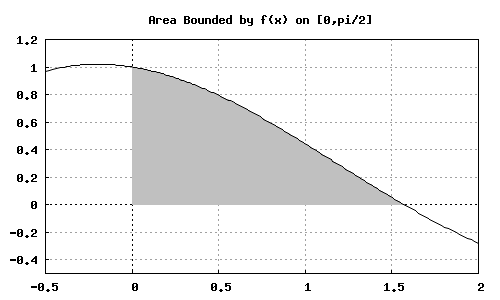
\includegraphics[width=3in]{example_3_1_1_2}
\end{exmp}

\line(1,0){60}
\linethickness{0.5mm}



\subsection{Area Bounded Between Two Functions}


To compute the area bounded \textit{between} two functions, we simply have to visualize an area element and write down $\mathrm{d}A$ in terms of the given functions.  Then we use the integral $A=\displaystyle \int \mathrm{d}A$ to add up all the area elements on the appropriate interval.


\begin{exmp}  Compute the area bounded between $f(x)=2-x^2$ and $g(x)=x$.\\
${}$\\

We start with a quick sketch:

\begin{verbatim}
(%i1) f(x):=2-x^2$
      g(x):=x$
(%i3) wxdraw2d(
      grid=true,
      xaxis=true,
      yaxis=true,
      xrange=[-2,2],
      yrange=[-2,2],
      title="Area bounded between f(x) and g(x).",
      color=black,
      key="f(x)",
       explicit(f(x),x,-2,2),
      color=red,
      key="g(x)",
      explicit(g(x),x,-2,2)
      );
\end{verbatim}

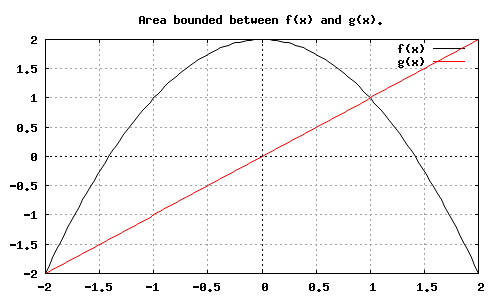
\includegraphics[width=3in]{example_3_1_2_1}

Now we determine the appropriate integration interval:  the bounded area occurs between the two intersections of our curves.

\begin{verbatim}
(%i4) solve(f(x)=g(x),x);
(%o4) [x=1,x=-2]
\end{verbatim}


Finally, we can visualize an area element on the integration interval and write down its formula.  Here, we use a thin rectangle to show an area element at $x=-0.5$:

\begin{verbatim}
(%i5) wxdraw2d(
      grid=true,
      xaxis=true,
      yaxis=true,
      xrange=[-2,2],
      yrange=[-2,2],
      title="Area bounded between f(x) and g(x).",
      color=red,
      border=false,
       rectangle([-0.5,g(-0.5)],[-0.45,f(-0.45)]),
      color=black,
       label(["dA",-0.33,1]),
      key="f(x)",
       explicit(f(x),x,-2,2),
      color=red,
      key="g(x)",
       explicit(g(x),x,-2,2)
      );
\end{verbatim}


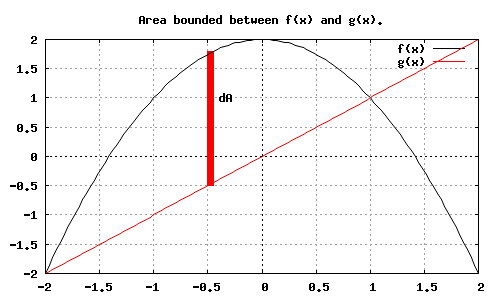
\includegraphics[width=3in]{example_3_1_2_2}


We see that the area element has a height of $f(x)-g(x)$, so we get $\mathrm{d}A=[f(x)-g(x)]\cdot \mathrm{d}x$.  We add up the area elements by computing the integral $A=\displaystyle \int  \mathrm{d}A=\displaystyle \int_{-2}^{1} [f(x)-g(x)]\ \mathrm{d}x $:

\begin{verbatim}
(%i6) float(integrate((f(x)-g(x)),x,-2,1));
(%o6) 4.5
\end{verbatim}

We obtain $A=4.5$ units.  We can also produce a filled plot of the area we have computed:

\begin{verbatim}
(%i7) wxdraw2d(
      grid=true,
      xaxis=true,
      yaxis=true,
      xrange=[-2,2],
      yrange=[-2,2],
      title="Area bounded between f(x) and g(x).",
      fill_color=grey,
       filled_func=true,
        filled_func=f(x),
        explicit(g(x),x,-2,1),
       filled_func=false,
     color=black,
     key="f(x)",
      explicit(f(x),x,-2,2),
     color=red,
     key="g(x)",
      explicit(g(x),x,-2,2)
     );
\end{verbatim}

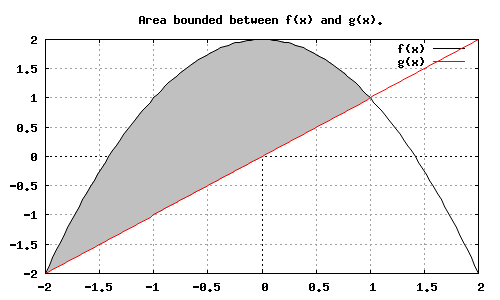
\includegraphics[width=3in]{example_3_1_2_3}

\end{exmp}

\line(1,0){60}
\linethickness{0.5mm}


\begin{exmp}  Compute the area bounded between $f(x)=\cosh{x}$ and $g(x)=5 \cos{3x}$.\\
${}$\\
We start with a sketch:

\begin{verbatim}
(%i8) f(x):=cosh(x)$
      g(x):=5*cos(3*x)$
      wxdraw2d(
      grid=true,
      xaxis=true,
      yaxis=true,
      xrange=[-4,4], 
      yrange=[-6,6],
      title="Area bounded between f(x) and g(x).",
      color=black,
      key="f(x)",
       explicit(f(x),x,-4,4),
      color=red,
      key="g(x)",
      explicit(g(x),x,-4,4)
      );
\end{verbatim}

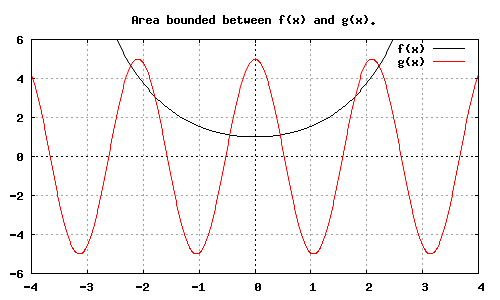
\includegraphics[width=3in]{example_3_1_3_1}

We see that both functions are even, so we can just find the area to the right of $x=0$ and double the result.  To verify that the functions are even:

\begin{verbatim}
(%i9) f(-x);
      g(-x);
(%o9) cosh(x)
(%o10) 5*cos(3*x)
\end{verbatim}

We have to keep in mind that we are no longer computing \textit{signed} area but \textit{geometric} area, which is always positive.  Thus, when $f(x)$ lies above $g(x)$, the area element is $[f(x)-g(x)]\cdot \mathrm{d}x$, but when $g(x)$ lies above $f(x)$, the area element becomes $[g(x)-f(x)]\cdot \mathrm{d}x$.  We have to split the integration interval into three pieces according to the intersections of $f(x)$ and $g(x)$, then we add up the areas and multiply by 2:

\begin{verbatim}
(%i11) x1:find_root(f(x)-g(x),0,1);
       x2:find_root(f(x)-g(x),1.5,2);
       x3:find_root(f(x)-g(x),2,2.5);
(%o11) 0.44947432956866
(%o12) 1.792473165779467
(%o13) 2.219127938640189
(%i14) ratprint:false$
       A1:float(integrate(g(x)-f(x),x,0,x1));
       A2:float(integrate(f(x)-g(x),x,x1,x2));
       A3:float(integrate(g(x)-f(x),x,x2,x3));
(%o14) 1.160865665363456
(%o15) 5.39123022939955
(%o16) 0.29427502144913
(%i17) A1+A2+A3;
(%o17) 6.846370916212132

(%i18) %*2;
(%o18) 13.69274183242426
\end{verbatim}

We obtain a total area $A\approx 13.7$.  We finish with a filled plot for the right half of the area:


\begin{verbatim}
(%i19) wxdraw2d(
       grid=true,
       xaxis=true,
       yaxis=true,
       xrange=[0,3],
       title="Area bounded between f(x) and g(x).",
       fill_color=grey,
        filled_func=true,
         filled_func=g(x),
         explicit(f(x),x,0,x1),
        filled_func=false,
        filled_func=true,
         filled_func=f(x),
         explicit(g(x),x,x1,x2),
        filled_func=false,
        filled_func=true,
         filled_func=g(x),
         explicit(f(x),x,x2,x3),
         filled_func=false,
        color=black,
        key="f(x)",
         explicit(f(x),x,0,3),
        color=red,
        key="g(x)",
         explicit(g(x),x,0,3)
        );
\end{verbatim}

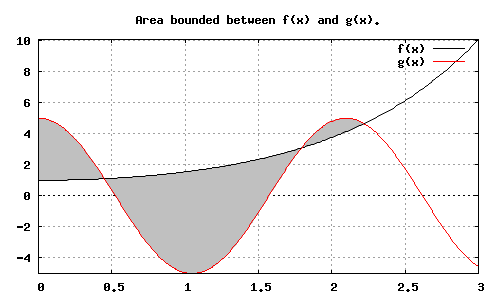
\includegraphics[width=3in]{example_3_1_3_2}

\end{exmp}

\line(1,0){60}
\linethickness{0.5mm}

\pagebreak








\pagebreak
\section{Solids of Revolution}\label{Solids of Revolution}

A \textbf{solid of revolution} is a three-dimensional object created by revolving the graph of a function $f(x)$ about an axis (usually the $x$ or $y$ axis). Solids of revolution have \textit{cylindrical symmetry}, making their volumes relatively easy to compute.  We use a physical integration approach by visualizing a small volume element $\mathrm{d}V$ and summing the elements with an integral:  $V=\displaystyle \int \mathrm{d}V$.  The cylindrical symmetry of a solid of revolution gives us two main options for choosing $\mathrm{d}V$:  the ``disk/washer'' method and the ``cylindrical shell'' method. \\

${}$\\

Note:  In the following examples, we use sets of \textit{parametric equations} to plot solids of revolution in \verb|wxdraw3d|.  The 3d graphs are a useful tool for visualization, but the mathematics required to plot them is more appropriate for students who have taken a multivariable calculus course.  We include all the code for the sake of completeness.

\subsection{Disks and Washers}

The ``disk/washer'' method uses volume elements made of thin cylindrical slices.  The thin slices are disks when the object is solid, and the slices are ``washers'' when the object has a hole along the symmetry axis.

\begin{exmp} Plot $f(x)=x^2$ and the solid of revolution obtained by rotating $f(x)$ on $[0,2]$ about the $x$-axis.  Include a disk $\mathrm{d}V$ in the plot.  Finally, formulate $\mathrm{d}V$ in terms of a single variable and use an integral to sum the volume elements.\\


\begin{verbatim}
(%i1) wxdraw2d(
      dimensions=[600,600],
      xrange=[0,3],
      yrange=[-4,4],
      xaxis=true,
      yaxis=true,
      xtics=false,
      ytics=false,
      line_width=2,
      title="f(x)=x^2 on [0,2]",
      color=black,
      explicit(x^2,x,0,2)
      );
(%i2) wxdraw3d(  
      axis_3d=false,
      dimensions=[600,600],
      view=[85,10],
      xrange=[0,3],
      yrange=[-4,4],
      zrange=[-4,4],
      xtics=false,
      ytics=false,
      ztics=false,
      color=black,
      nticks=600,
      line_width=2,
       parametric(t,0,0,t,0,3),
       parametric(0,t,0,t,-4,4),
       parametric(0,0,t,t,-4,4),
      color=dark_grey,
       parametric_surface(r,r^2*cos(t),r^2*sin(t),r,0,2,t,0,2*%pi),
      color=black,
       parametric_surface(r,r^2*cos(t),r^2*sin(t),r,1.3,1.4,t,0,2*%pi),
      color=dark_red,
       parametric_surface(1.4,u^2*cos(t),u^2*sin(t),u,0,1.4,t,0,2*%pi)
      );
\end{verbatim}

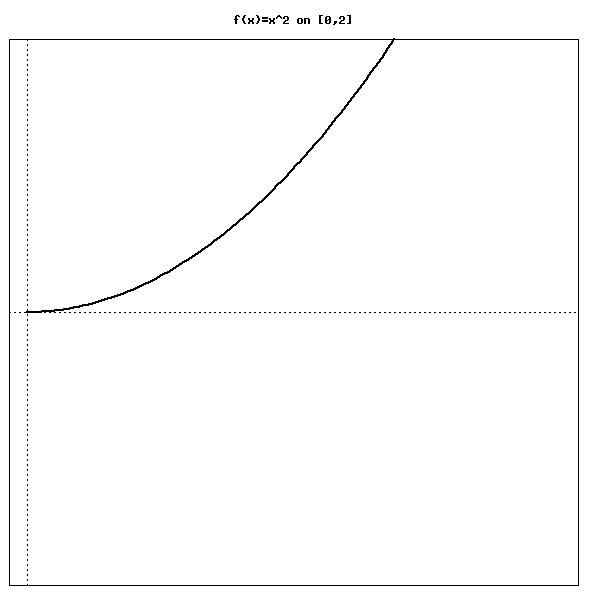
\includegraphics[width=2.7in]{example_3_2_1_1}
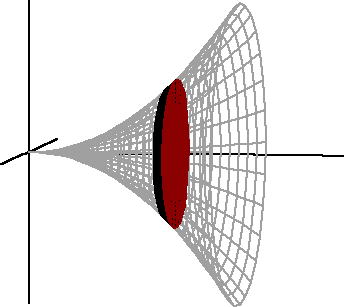
\includegraphics[width=2.7in]{example_3_2_1_2}


Although the $z$-axis is technically pointing up in this picture, the symmetry of the graph allows us to look at the vertical axis as $y$.  The curved surface is ``swept out'' as we rotate $y=x^2$ about the $x$-axis.  \\
${}$\\
$\mathrm{d}V$ is included in black, and we say it has a (horizontal) thickness of $\mathrm{d}x$ and a radius of $x^2$ for the particular $x$ location of the disk ($x^2$ is the distance from the $x$-axis to a point on the original curve).  The volume of the disk is the product of the area of the base and the thickness, so  $\mathrm{d}V=\pi\cdot (x^2)^2\cdot \mathrm{d}x$.  Now we can set up the volume integral with the limits of integration corresponding to $x$: 
\[V=\int \mathrm{d}V=\int_0^2 \pi\cdot x^4\ \mathrm{d}x\]

This integral isn't too hard to compute by hand, but we use wxMaxima for practice:\\

\begin{verbatim}
(%i3) integrate(%pi*x^4,x,0,2);
(%o3) (32*%pi)/5
(%i4) float(%);
(%o4) 20.10619298297468
\end{verbatim}

The volume comes out to $V=\frac{32\pi}{5}\approx 20.1$ units.

\end{exmp}

\line(1,0){60}
\linethickness{0.5mm}


\begin{exmp} Plot $f(x)=x^2$ and the solid of revolution obtained by rotating $f(x)$ on $[0,2]$ about the $y$-axis.  Include a disk $\mathrm{d}V$ in the plot.  Finally, formulate $\mathrm{d}V$ in terms of a single variable and use an integral to sum the volume elements.

\begin{verbatim}
(%i5) wxdraw2d(
       dimensions=[600,600],
       xrange=[-3,3],
       yrange=[0,9],
       xaxis=true,
       yaxis=true,
       xtics=false,
       ytics=false,
       line_width=2,
       title="f(x)=x^2 on [0,2]",
       color=black,
       explicit(x^2,x,0,2)
       );

(%i6) wxdraw3d(  
      axis_3d=false,
      dimensions=[600,600],
      view=[85,10],
      xrange=[-3,3],
      yrange=[-3,3],
      zrange=[0,9],
      xtics=false,
      ytics=false,
      ztics=false,
      color=black,
      nticks=600,
      line_width=2,
       parametric(t,0,0,t,-3,3),
       parametric(0,t,0,t,-3,3),
       parametric(0,0,t,t,0,6), 
      color=dark_grey,
       parametric_surface(r*cos(t),r*sin(t),r^2,r,0,2,t,0,2*%pi),
      color=black,
       parametric_surface(r*cos(t),r*sin(t),r^2,r,1.3,1.4,t,0,2*%pi),
      color=dark_red,
       parametric_surface(r*cos(t),r*sin(t),1.4^2,r,0,1.4,t,0,2*%pi)
      );
\end{verbatim}

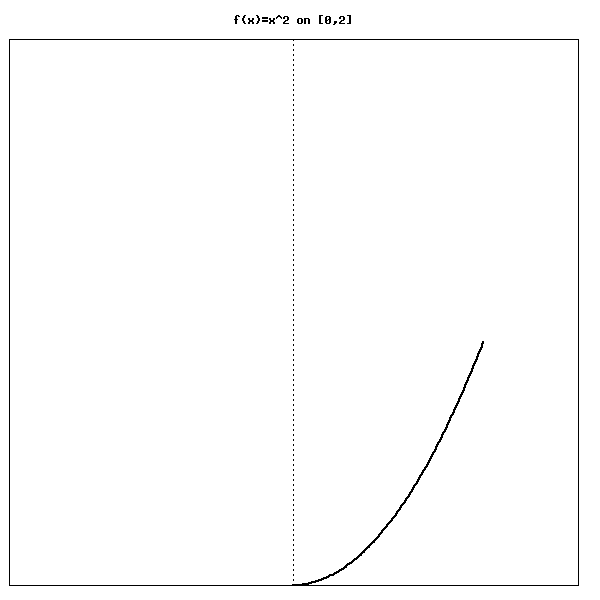
\includegraphics[width=2.7in]{example_3_2_2_1}
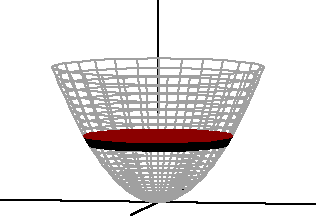
\includegraphics[width=2.7in]{example_3_2_2_2}


Again, it is easier to produce a plot with $f(x)$ revolved about the $z$-axis, but we can view it as the $y$-axis:  we produced the plot simply to aid our intuition.  This time, the thickness of the disk is $\mathrm{d}y$.  The disk is located at a vertical position of $y$, where the radius is given as $x=\sqrt{y}$, so the volume of the disk is $\mathrm{d}V=\pi\cdot (\sqrt{y})^2\cdot \mathrm{d}y$.  We set up the volume integral with the limits of integration corresponding to $y$ (as $x$ goes from 0 to 2, $y=x^2$ goes from 0 to 4):

\[V=\int \mathrm{d}V = \int_0^4 \pi\cdot y\ \mathrm{d}y\]

Again, the integral is simple to compute by hand, but we opt to use wxMaxima:

\begin{verbatim}
(%i7) integrate(y,y,0,4);
(%o7) 8
\end{verbatim}

The volume comes out to $V=8$ units.



\end{exmp}

\line(1,0){60}
\linethickness{0.5mm}

\begin{exmp} Plot the region bounded between $f(x)=0.3\cdot x$ and $g(x)=\sin{x}$, then plot the solid of revolution obtained by rotating this region about the $x$-axis, including a ``washer'' volume element $\mathrm{d}V$.  Finally, set up and compute the volume integral for the solid.\\

${}$\\

The plot of bounded area between $f(x)$ and $g(x)$ requires us to find the intersections by solving $0.3\cdot x=\sin{x}$ with \verb|find_root|.  We use symmetry to infer the second intersection from the first.  We plot the area using \verb|filled_func| for the shading:

\begin{verbatim}
(%i8) kill(all)$

(%i1) f(x):=0.3*x$
      g(x):=sin(x)$
(%i3) find_root(f(x)-g(x),x,1,4);
(%o3) 2.356441149856161

(%i4) wxdraw2d(
      xaxis=true,
      yaxis=true,
      xtics=false,
      ytics=false,
      dimensions=[600,600],
      xrange=[-%pi,%pi],
      yrange=[-1.2,1.2],
      title="Area bounded between f(x) and g(x)",
      fill_color=grey,
       filled_func=true,
        filled_func=f(x),
        explicit(g(x),x,-2.356,0),
       filled_func=false,
       filled_func=true,
        filled_func=g(x),
        explicit(f(x),x,0,2.356),
       filled_func=false,
      line_width=2,
      color=black,
      key="f(x)",
       explicit(f(x),x,-%pi,%pi),
      color=red,
      key="g(x)",
       explicit(g(x),x,-%pi,%pi)
      );
\end{verbatim}

Again, plotting the solid of revolution is more appropriate for students of multivariable calculus, but we include the code for reference:

\begin{verbatim}
(%i5)wxdraw3d(
     axis_3d=false,
     dimensions=[600,600],
     view=[85,10],
     xrange=[-%pi,%pi],
     yrange=[-1.2,1.2],
     zrange=[-1.2,1.2],
     xtics=false,
     ytics=false,
     ztics=false,
     color=black,
     nticks=200,
     line_width=2,
      parametric(t,0,0,t,-%pi,%pi),
      parametric(0,t,0,t,-1.2,1.2),
      parametric(0,0,t,t,-1.2,1.2),    
     color=grey,
     transparent=true,
      parametric_surface(r, g(r)*sin(t),g(r)*cos(t),r,-2.356,2.356,t,
      0,2*%pi),
     transparent=false,
     color=dark_grey,
      parametric_surface(r, f(r)*sin(t), f(r)*cos(t),r,-2.356, 2.356,t,
      0,2*%pi),
     color=black,
      parametric_surface(r, g(r)*sin(t), g(r)*cos(t),r,1.5,1.6,t,0,2*%pi),
     color=dark_red,
      parametric_surface(1.6, u*sin(t),u*cos(t),u,f(1.6),g(1.6),t,0,2*%pi)
     );
\end{verbatim}


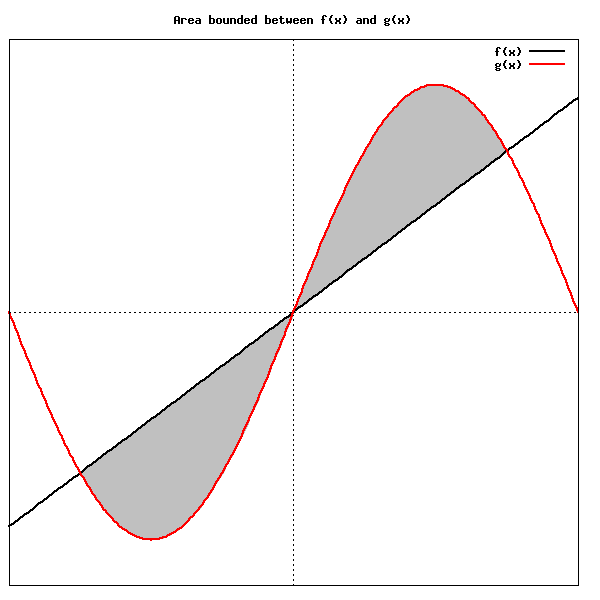
\includegraphics[width=2.7in]{example_3_2_3_1}
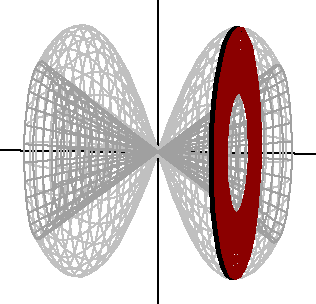
\includegraphics[width=2.7in]{example_3_2_3_2}

${}$\\

For the volume calculation, we can just find the volume of the right half and multiply by 2.  The volume of the ``washer'' is still given by the product of area and thickness, and the area of the base is just the area of the outer circle less the area of the inner circle:  $A=\pi\cdot r_{outer}^2-\pi\cdot r_{inner}^2$. Thus $\mathrm{d}V =\left( \pi\cdot (\sin{x})^2 - \pi\cdot (0.3\cdot x)^2 \right)\cdot \mathrm{d}x$. Finally, we set up the volume integral:

\[V=\int \mathrm{d}V = 2\cdot \int_0^{2.356} \pi\cdot (\sin{x})^2 - \pi\cdot (0.3\cdot x)^2 \ \mathrm{d}x\]

${}$\\
Computing the integral in wxMaxima:

\begin{verbatim}
(%i6) ratprint:false$
(%i7) float(2*integrate(%pi*(sin(x))^2-%pi*(0.3*x)^2, x, 0, 2.356));
(%o7) 6.507331412313022
\end{verbatim}

We obtain a volume of $V\approx 6.5$ units.


\end{exmp}

\line(1,0){60}
\linethickness{0.5mm}
\pagebreak



\subsection{Cylindrical Shells}

A solid of revolution can also be decomposed into volume elements given by nested cylindrical shells.  The volume of a cylindrical shell of height $h$, radius $r$, and thickness $\mathrm{d}r$ is found by ``unrolling'' the shell into a rectangular slab.  When a shell is unrolled, the length is $2\pi r$ (the circumference of the original shell).   Thus, we use $\mathrm{d}V = 2\pi r\cdot h\cdot \mathrm{d}r$ whenever we decompose a solid into cylindrical shells.

\begin{exmp} Plot the area bounded by $f(x)=\cosh{x}$ on $[-2,2]$, then plot the solid formed by revolving this area about the $y$-axis.  Include a picture of a thin cylindrical shell volume element.  Finally, set up and compute the volume integral.\\

${}$\\

We start by defining $f(x)$ and plotting the shaded area:

\begin{verbatim}
(%i8) kill(all)$
(%i1) f(x):=cosh(x)$
      wxdraw2d(
      xaxis=true,
      yaxis=true,
      xtics=false,
      ytics=false,
      dimensions=[600,600],
      xrange=[-2.5,2.5],
      yrange=[-0.1,4],
      title="Area under f(x)=cosh(x)",
      fill_color=grey,
       filled_func=true,
        filled_func=f(x),
        explicit(0,x,-2.0,2.0),
       filled_func=false,
      line_width=2,
      color=black,
       explicit(f(x),x,-2.5,2.5)
      );
\end{verbatim}


Again, the code for the 3d plot is included for reference:

\begin{verbatim}
(%i3) wxdraw3d(  
      axis_3d=false,
      dimensions=[600,600],
      view=[75,10],
      xrange=[-2.5,2.5],
      yrange=[-2.5,2.5],
      zrange=[0,4],
      xtics=false,
      ytics=false,
      ztics=false,
      color=black,
      nticks=600,
      line_width=2,
       parametric(t,0,0,t,-2.5,2.5),
       parametric(0,t,0,t,-2.5,2.5),
       parametric(0,0,t,t,-0.1,4), 
      color=dark_grey,
       parametric_surface(r*cos(t),r*sin(t),cosh(r),r,0,2,t,0,2*%pi),
      color=grey,
       parametric_surface(2*cos(t),2*sin(t),u,t,0,2*%pi,u,0,cosh(2)),
      color=black,
       parametric_surface(1.3*cos(t),1.3*sin(t),u,u,0,cosh(1.3),t,0,2*%pi),
      color=dark_red,
       parametric_surface(r*cos(t),r*sin(t),cosh(1.3),r,1.2,1.3,t,0,2*%pi)
      );
\end{verbatim}

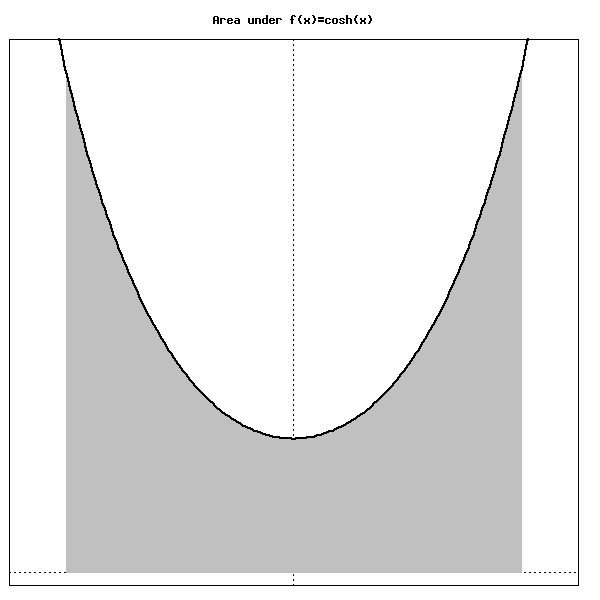
\includegraphics[width=2.7in]{example_3_2_4_1}
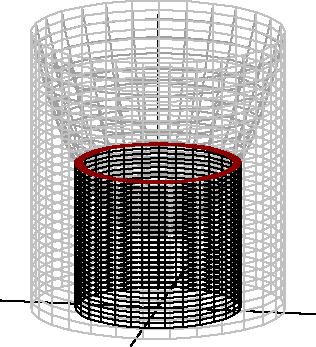
\includegraphics[width=2.5in]{example_3_2_4_2}

${}$\\
The radius of the cylindrical shell is $x$, the height is $\cosh{x}$ and the thickness is $\mathrm{d}x$.  When we unroll the shell, we get a slab with length $2\pi x$, height $\cosh{x}$ and thickness $\mathrm{d}x$, so $\mathrm{d}V=2\pi x\cdot \cosh{x}\ \mathrm{d}x$.  Now we can set up the volume integral and finish the calculation:\\

\[V=\int \mathrm{d}V = \int_0^2 2\pi x\cdot \cosh{x}\ \mathrm{d}x\]

\begin{verbatim}
(%i4) float(integrate(2*%pi*x*cosh(x),x,0,2));
(%o4) 28.22108466978007
\end{verbatim}

We obtain a volume $V\approx 28.2$ units.


\end{exmp}

\line(1,0){60}
\linethickness{0.5mm}
\pagebreak

\pagebreak
\section{Arc Length}\label{Arc Length}

\subsection{As a Limiting Process}

The arc length of a curve $f(x)$ on can be viewed as a limiting process:  we break $[a,b]$ into $n$ sub-intervals at $x_0,x_1,...,x_n$, then we compute the line segments connecting all the adjacent points on the curve $(x_{i},f(x_{i}))$ and $(x_{i+1},f(x_{i+1}))$.  Finally, we add the lengths of all the line segments to obtain an approximation to the arc length of $f(x)$ on $[a,b]$.  Clearly, as $n$ becomes larger, the approximation becomes more accurate.

\begin{exmp} Plot the $n=2$, $n=5$, $n=10$ and $n=20$ arc length approximations for $f(x)=\displaystyle \frac{e^{x}}{x^3}$ on $[1,5]$.  Compute the numerical value for each approximation.  Finally, improve on the accuracy of your approximation by computing the arc length for $n=1000$.\\
${}$\\
First, we define $f(x)$, a function \verb|LINE(a,b,c,d)| computing the equation of a line connecting two arbitrary points $(a,b)$ and $(c,d)$, and a function \verb|LENGTH(a,b,c,d)| to compute the length of a line segment connecting $(a,b)$ and $(c,d)$:\\

\begin{verbatim}
(%i1) f(x):=(e^x)/(x^3)$
      SLOPE(a,b,c,d):=(d-b)/(c-a)$
      LINE(a,b,c,d):=SLOPE(a,b,c,d)*(x-a)+b$
      LENGTH(a,b,c,d):=sqrt((c-a)^2+(d-b)^2)$
\end{verbatim}

The next step is to define $x_i$ as a function of $i$ and $n$.  We use $\Delta x=(5-1)/n$:

\begin{verbatim}
(%i5) delx(n):=(5-1)/n$
      x(n,i):=1+(i)*delx(n)$
\end{verbatim}

We assign each value of $n$ and use \verb|makelist| to generate line segments in the correct form for \verb|wxdraw2d|:

\begin{verbatim}
(%i7) n:2$
      SEGMENTS2:makelist(explicit(LINE(x(n,i),f(x(n,i)),
      x(n,i+1),f(x(n,i+1))),x,x(n,i),x(n,i+1)),i,0,n-1)$
(%i9) n:5$
      SEGMENTS5:makelist(explicit(LINE(x(n,i),f(x(n,i)),
      x(n,i+1),f(x(n,i+1))),x,x(n,i),x(n,i+1)),i,0,n-1)$
(%i11) n:10$
       SEGMENTS10:makelist(explicit(LINE(x(n,i),f(x(n,i)),
       x(n,i+1),f(x(n,i+1))),x,x(n,i),x(n,i+1)),i,0,n-1)$
(%i13) n:20$
       SEGMENTS20:makelist(explicit(LINE(x(n,i),f(x(n,i)),
       x(n,i+1),f(x(n,i+1))),x,x(n,i),x(n,i+1)),i,0,n-1)$
\end{verbatim}

Finally, we produce a plot of each approximation:

\begin{verbatim}
(%i15) wxdraw2d(
       grid=true,
       xaxis=true,
       yaxis=true,
       xrange=[0.5,5.5],
       yrange=[0,3],
       title="n=2 arc length approximation",
       color=black,
       line_type=dots,
        explicit(f(x),x,1,5),
       line_width=2,
       color=red,
        SEGMENTS2
       );

(%i16) wxdraw2d(
       grid=true,
       xaxis=true,
       yaxis=true,
       xrange=[0.5,5.5],
       yrange=[0,3],
       title="n=5 arc length approximation",
       color=black,
       line_type=dots,
        explicit(f(x),x,1,5),
       line_width=2,
       color=red,
        SEGMENTS5
       );

(%i17) wxdraw2d(
       grid=true,
       xaxis=true,
       yaxis=true,
       xrange=[0.5,5.5],
       yrange=[0,3],
       title="n=10 arc length approximation",
       color=black,
       line_type=dots,
        explicit(f(x),x,1,5),
       line_width=2,
       color=red,
        SEGMENTS10
       );

(%i18) wxdraw2d(
       grid=true,
       xaxis=true,
       yaxis=true,
       xrange=[0.5,5.5],
       yrange=[0,3],
       title="n=20 arc length approximation",
       color=black,
       line_type=dots,
        explicit(f(x),x,1,5),
       line_width=2,
       color=red,
        SEGMENTS20
       );
\end{verbatim}



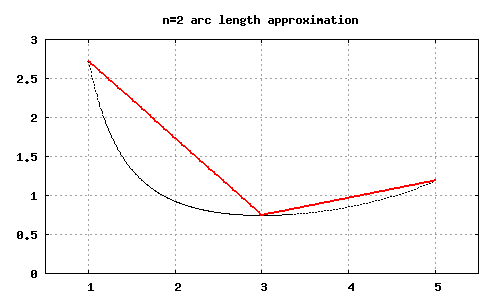
\includegraphics[width=2.7in]{example_3_3_1_1}
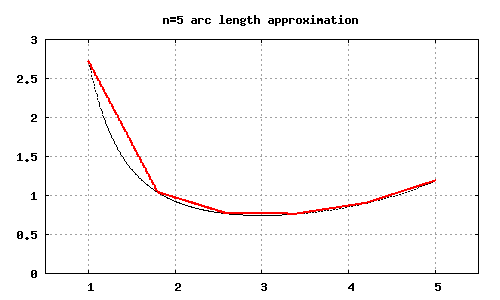
\includegraphics[width=2.7in]{example_3_3_1_2}

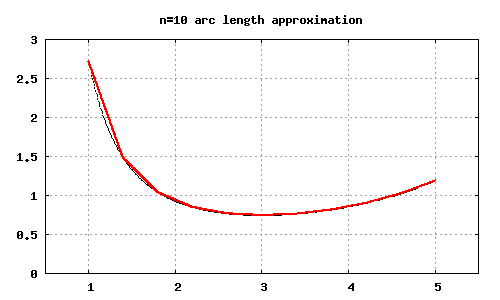
\includegraphics[width=2.7in]{example_3_3_1_3}
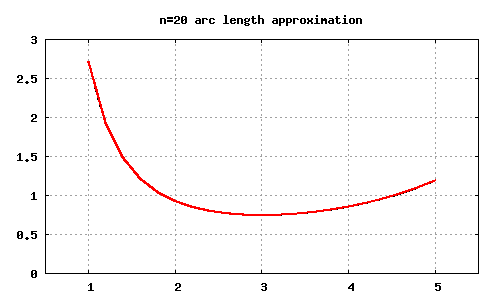
\includegraphics[width=2.7in]{example_3_3_1_4}

${}$\\

Now we can compute the numerical values of all the approximations, including $n=1000$:

\begin{verbatim}
(%i19) n:2$
       APPROX2:float(sum(LENGTH(x(n,i),f(x(n,i)),x(n,i+1),f(x(n,i+1))),
       i,0,n-1));

(%o20) 4.858925140077406

(%i21) n:5$
       APPROX5:float(sum(LENGTH(x(n,i),f(x(n,i)),x(n,i+1),f(x(n,i+1))),
       i,0,n-1));

(%o22) 5.168139881862706

(%i23) n:10$
       APPROX10:float(sum(LENGTH(x(n,i),f(x(n,i)),x(n,i+1),f(x(n,i+1))),
       i,0,n-1));

(%o24) 5.213749217721892

(%i25) n:20$
       APPROX20:float(sum(LENGTH(x(n,i),f(x(n,i)),x(n,i+1),f(x(n,i+1))),
       i,0,n-1));

(%o26) 5.224566917514401

(%i27) n:1000$
       APPROX1000:float(sum(LENGTH(x(n,i),f(x(n,i)),x(n,i+1),f(x(n,i+1))),
       i,0,n-1));

(%o28) 5.228147830313162
\end{verbatim}

We see that the arc length is approaching a limiting value of about 5.23.
\end{exmp}

\line(1,0){60}
\linethickness{0.5mm}



\begin{exmp} Estimate $\pi$ by using an $n=1000$ arc length approximation to compute the arc length of a semicircle of radius 1.  What percent error is obtained?\\
${}$\\
The explicit equation for the upper half of the unit circle is $f(x)=\sqrt{1-x^2}$.  The circumference of the unit circle is $2\pi r=2\pi$, so the semicircle should have an arc length of $\pi$.  We copy the relevant code from the last example, using an interval $[-1,1]$, so that \verb|delx(n)=2/n| and \verb|x(n,i)| starts at $-1$:

\begin{verbatim}
(%i29) kill(all)$

       f(x):=sqrt(1-x^2)$
       LENGTH(a,b,c,d):=sqrt((c-a)^2+(d-b)^2)$
       delx(n):=2/n$
       x(n,i):=-1+(i)*delx(n)$
       n:1000$
       float(sum(LENGTH(x(n,i),f(x(n,i)),x(n,i+1),f(x(n,i+1))),i,0,n-1));
(%o6) 3.141566356216483

(%i7) float(100*(%-%pi)/%pi);
(%o7) -8.3707139052572146*10^-4
\end{verbatim}

Our approximation of $\pi$ misses by only $.0008$\verb|%|.


\end{exmp}

\line(1,0){60}
\linethickness{0.5mm}

\pagebreak
\subsection{As a Physical Integral}

We can also approach the arc length problem symbolically by visualizing a small arc length element $\mathrm{d}s$ on the graph of $f(x)$:\\

${}$\\




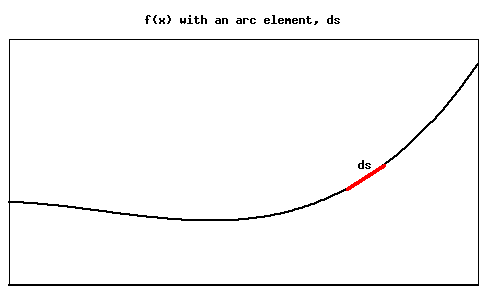
\includegraphics[width=2.7in]{figure_3_3_2_1} %zoomed out
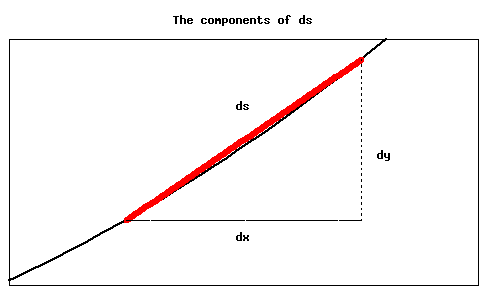
\includegraphics[width=2.7in]{figure_3_3_2_2} %zoomed in

When we zoom in on $\mathrm{d}s$, we see that it can be decomposed into $x$ and $y$ components, and we apply the pythagorean theorem to obtain $\mathrm{d}s=\sqrt{(\mathrm{d}x)^2+(\mathrm{d}y)^2}$. \\
${}$\\



Finally, we factor $\mathrm{d}x$ out of this expression to obtain $\mathrm{d}s=\sqrt{1+\left(\frac{\mathrm{d}y}{\mathrm{d}x}\right)^2}\cdot \mathrm{d}x$
${}$, and we set up arc length as an integral:

\[S=\int \mathrm{d}s = \int_a^b \sqrt{1+(f'(x))^2}\ \mathrm{d}x\]

In practice, this integral can rarely be computed by hand, but it is simple to obtain a numerical approximation in wxMaxima.\\





\begin{exmp} Compute the arc length of $f(x)=\displaystyle \frac{e^{x}}{x^3}$ on $[1,5]$ and compare with the $n=1000$ approximation obtained in Example 3.3.1

\begin{verbatim}

(%i8) f(x):=%e^x/(x^3);
(%o8) f(x):=%e^x/x^3
(%i9) f_prime:diff(f(x),x);
(%o9) %e^x/x^3-(3*%e^x)/x^4
(%i10) integrate(sqrt(1+(f_prime)^2),x,1,5);
(%o10) integrate(sqrt((%e^x/x^3-(3*%e^x)/x^4)^2+1),x,1,5)
\end{verbatim}

wxMaxima repeats the integral to us, indicating that it can't find an analytical solution.  We use \verb|quad_qag| to get an approximation:

\begin{verbatim}
(%i36) quad_qag(sqrt(1+(f_prime)^2),x,1,5,1);
(%o36) [5.228149260997872,6.6513611026699459*10^-9,75,0]
\end{verbatim}

We find that the arc length is about 5.23, as before.  In fact, the two answers agree in the first five decimal places!

\end{exmp}

\line(1,0){60}
\linethickness{0.5mm}
\pagebreak

\pagebreak
\section{Surface Area}\label{Surface Area}

A surface area of revolution can be computed by slicing it into thin ribbons.  Each ribbon forms an area element, $\mathrm{d}A$:\\

\begin{center}
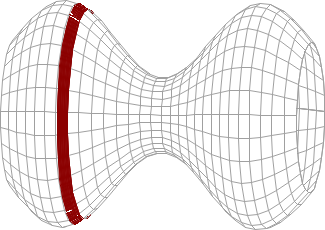
\includegraphics[width=3in]{figure_3_4_1}
\end{center}

We ``unroll'' $\mathrm{d}A$ to find its area:  the width of each ribbon is given by an arc element, $\mathrm{d}s$, of the curve we revolved, and the length is found by applying the formula for the circumference of a circle.  Once $\mathrm{d}A$ is phrased entirely in terms  of one variable, we integrate to sum the area elements.\\
${}$\\
Note:  once again, the 3d plots are more appropriate for students who have seen multivariable calculus, but we include them here for completeness.

\begin{exmp} Compute the area of the surface created by revolving $f(x)=\cosh{x}$ about the $x$-axis on $[-2,2]$.  \\
${}$\\
We begin by producing plots of $f(x)$ and the corresponding surface of revolution:

\begin{verbatim}
(%i1) wxdraw2d(
      dimensions=[600,600],
      xrange=[-2.2,2.2],
      yrange=[-4,4],
      xaxis=true,
      yaxis=true,
      xtics=false,
      ytics=false,
      line_width=2,
      title="f(x)=cosh(x) on [-2,2]",
      color=black,
      explicit(cosh(x),x,-2,2)
      );

(%i2) wxdraw3d(  
      axis_3d=false,
      dimensions=[600,600],
      view=[85,10],
      xrange=[-2.2,2.2],
      yrange=[-4,4],
      zrange=[-4,4],
      xtics=false,
      ytics=false,
      ztics=false,
      color=black,
      line_width=2,
       parametric(t,0,0,t,-2.2,2.2),
       parametric(0,t,0,t,-4,4),
       parametric(0,0,t,t,-4,4),
      nticks=600,
      surface_hide=true,
      wired_surface=true,
      color=dark_grey,
       parametric_surface(r,cosh(r)*cos(t),cosh(r)*sin(t),r,-2,2,t,0,2*%pi),
      color=dark_red,
       parametric_surface(r,1.01*cosh(r)*cos(t),1.01*cosh(r)*sin(t),
       r,1,1.2,t,0,2*%pi)
      );
\end{verbatim}

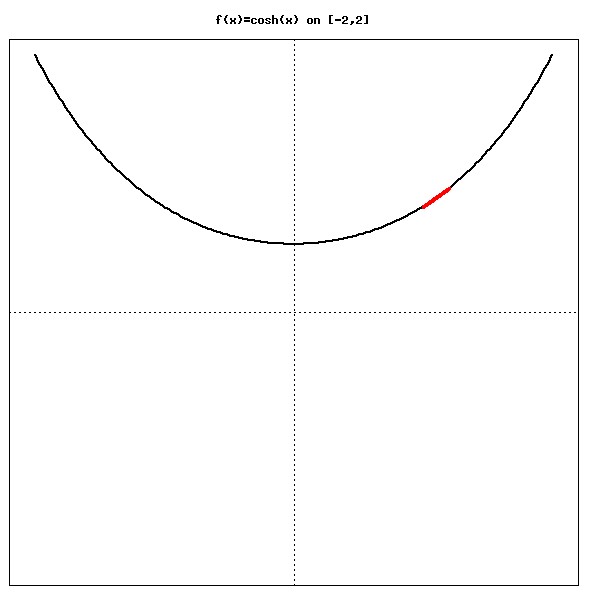
\includegraphics[width=2.7in]{example_3_4_1_1}
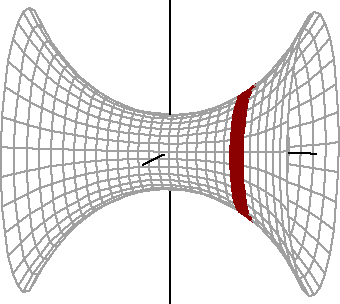
\includegraphics[width=2.7in]{example_3_4_1_2}

${}$\\
${}$\\

$\mathrm{d}s$ is a small element of arc on the graph of $f(x)=\cosh{x}$.  Again, we phrase $\mathrm{d}s$ in terms of $f'(x)$: $\mathrm{d}s=\sqrt{(\mathrm{d}x)^2+(\mathrm{d}y)^2}
=\sqrt{1+(\frac{\mathrm{d}y}{\mathrm{d}x})^2}\cdot \mathrm{d}x$.  Since $\cosh{x}$ is the radius of the area element at $x$, we can write the length of the ``unrolled'' area element as $2\pi\cdot \cosh{x}$.  We use wxMaxima to compute the formula for the area element $\mathrm{d}A$ entirely in terms of $x$:

\begin{verbatim}
(%i3) f(x):=cosh(x)$
      dels:sqrt(1+(diff(f(x),x))^2)$
      delA:2*%pi*f(x)*dels;
\end{verbatim}
\verb|(%o5)  | $2\,\pi \,\mathrm{cosh}\left( x\right) \,\sqrt{{\mathrm{sinh}\left( x\right) }^{2}+1}$

${}$\\

Finally, we add up all the surface area elements using an integral:  \[A=\int \mathrm{d}A= \int_{-2}^{2} 2\pi\cdot \cosh{x} \sqrt{(\sinh{x})^2+1}\ \mathrm{d}x\]

\begin{verbatim}
(%i6) integrate(%,x,-2,2);
(%o6) (%e^(-4)*(%e^8+8*%e^4-1)*%pi)/2
(%i7) float(%);
(%o7) 98.30017399792946
\end{verbatim}

We obtain a surface area of about 98.3 units.

\end{exmp}

\line(1,0){60}
\linethickness{0.5mm}

\begin{exmp} Compute the area of the surface obtained by revolving $f(x)=\sin{3x}+x$ about the $y$-axis on $[0,1.9]$.\\

${}$\\

Again, we start with the 2d and 3d plots:

\begin{verbatim}
(%i8) f(x):=sin(3*x)+x$
      wxdraw2d(
      dimensions=[600,600],
      xrange=[-2.2,2.2],
      yrange=[0,3],
      xaxis=true,
      yaxis=true,
      xtics=false,
      ytics=false,
      line_width=2,
      title="f(x)=sin(3x)+x on [0,1.9]",
      color=black,
      explicit(f(x),x,0,1.9),
      line_width=3,
      color=red,
      explicit((f(1.8)-f(1.7))/.1*(x-1.7)+f(1.7),x,1.7,1.8)
      );

(%i9) wxdraw3d(  
      axis_3d=false,
      dimensions=[600,600],
      view=[85,10],
      xrange=[-2.2,2.2],
      yrange=[-2.2,2.2],
      zrange=[0,3],
      xtics=false,
      ytics=false,
      ztics=false,
      color=black,
      line_width=2,
       parametric(t,0,0,t,-2.2,2.2),
       parametric(0,t,0,t,-2.2,2.2),
       parametric(0,0,t,t,0,3),
      nticks=600,
      surface_hide=true,
      wired_surface=true,
      color=dark_grey,
       parametric_surface(r*cos(t),r*sin(t),f(r),r,0,1.9,t,0,2*%pi),
      color=dark_red,
        parametric_surface(r*cos(t),r*sin(t),f(r),r,1.7,1.8,t,0,2*%pi)
      );
\end{verbatim}

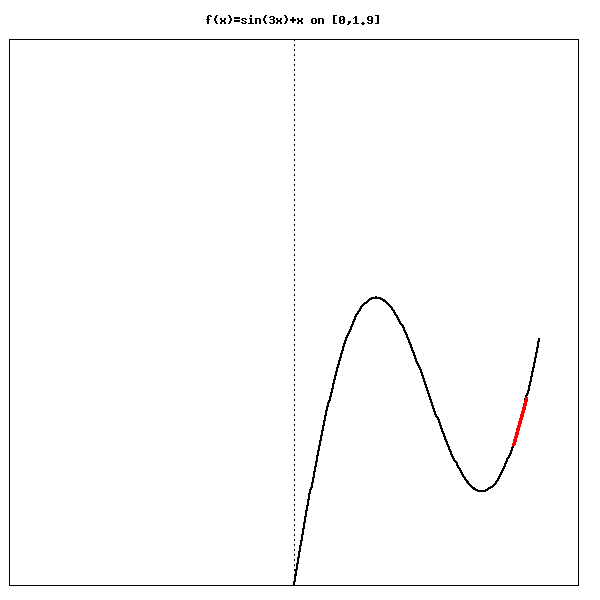
\includegraphics[width=2.7in]{example_3_4_2_1}
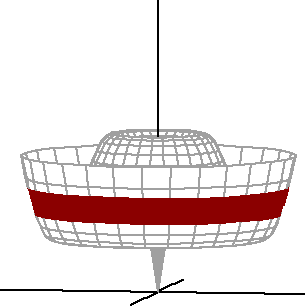
\includegraphics[width=2.7in]{example_3_4_2_2}

${}$\\

Once again, we write $\mathrm{d}s=\sqrt{1+(f'(x))^2}\ \mathrm{d}x$.  This time, each ring has a radius of $x$, so $\mathrm{d}A$ has a length of $2\pi\cdot x$.  We assemble $\mathrm{d}A$ in wxMaxima:

\begin{verbatim}
(%i10) sqrt(1+(diff(f(x),x))^2)*2*%pi*x;
\end{verbatim}
\verb|(%o10)  |$2\,\pi \,x\,\sqrt{{\left( 3\,\mathrm{cos}\left( 3\,x\right) +1\right) }^{2}+1}$\\
${}$\\
Finally, we add up all the area elements with an integral:
$$A=\int \mathrm{d}A = \int_0^{1.9} 2\,\pi \,x\,\sqrt{{\left( 3\,\mathrm{cos}\left( 3\,x\right) +1\right) }^{2}+1}\ \mathrm{d}x$$

${}$\\

When we try \verb|integrate|, wxMaxima fails to produce an answer, so we find a decimal approximation using \verb|quad_qag|:

\begin{verbatim}
(%i11) quad_qag(%,x,0,1.9,1);
(%o11) [22.52375662706631,1.6729090642515012*10^-7,195,0]
\end{verbatim}

We find a surface area $A\approx 22.5$ units.


\end{exmp}

\line(1,0){60}
\linethickness{0.5mm}
\pagebreak


\section{Module 3 Exercises}\label{Module 3 Exercises}

\begin{enumerate}

\item  Compute a decimal approximation for the signed area bounded by $f(x)=-x^2+2x$ on $[0,4]$.  Produce a shaded plot, using red for the positive area contribution and blue for the negative area contribution.

\item  Compute a decimal approximation for the area bounded between $f(x)=\sqrt{1-x^2}$ and $g(x)=\cos{(\frac{\pi}{2} x)}$.  You can use symmetry to streamline your work, but you should include the proper algebraic argument to justify the use of symmetry.  Produce a filled plot to illustrate the area you computed.

\item  Use a plot to investigate the graphs of $f(x)=(x-3)(x-2)(x-1)x(x+1)(x+2)(x+3)$ and $g(x)=e^x$.  Use wxMaxima to find all the intersections of these two functions, then compute the area bounded between them.  As in Example 3.1.3, you must be careful to make every area contribution in your calculation positive by choosing the correct difference of functions in each area integral.



\item Compute the volume of the solid created by revolving $f(x)=\cos{x}$ on $[0,\pi]$ about the $y$-axis.  Note:  since we are working on the ``agreed-upon'' domain restriction for the cosine function, we can ignore the warning that ``some solutions may be lost''.
  \begin{enumerate}
   \item Use the disk method.  Make sure to explicitly state the volume element $\mathrm{d}V$ before adding up the elements with an integral.
   \item Use the cylindrical shell method.  Make sure to explicitly state the volume element $\mathrm{d}V$ before adding up the elements with an integral.
   \item * Use \verb|wxdraw3d| to make plots of the solid together with each type of volume element.
  \end{enumerate}

\item Repeat the last example for revolution about the $x$ axis instead of the $y$ axis.

\item Make a shaded plot for the region bounded by $f(x)=1+0.5x$ and $g(x)=x$ on $[0,2]$.
 \begin{enumerate}
  \item  Use the washer method to compute the volume of the solid obtained by revolving this region about the $y$-axis.
  \item  Use the washer method to compute the volume of the solid obtained by revolving the region about the $x$-axis.
  \item * Use \verb|wxdraw3d| to make plots of each solid, including a volume element.
 \end{enumerate}

\item Make a shaded plot for the region bounded by $f(x)=\sin{x}$ and $g(x)=\cos{x}$ between their first two intersections on $[0,\frac{3\pi}{2}]$.  Use the washer method to compute the volume of the solid obtained by revolving this region about the $y$-axis.  Note: while the cosine is constrained to its standard domain restriction of $[0,\pi]$, the sine function is \textit{not}.  You will have to think carefully about how to adjust the outer radius on $[\frac{\pi}{2},\frac{3\pi}{2}]$.  Verify that the same answer is obtained using the cylindrical shell method.

\item Compute the arc-length for the function $f(x)=\sin{x}$ on $[0,2\pi]$ using two different methods:
 \begin{enumerate}
  \item Use a limiting process with $n=4,8,16,32,64$ sub-intervals, including plots of each approximation.  
  \item Use the integral formula for arc-length to compute a decimal approximation.
  \item Compute a percent error comparing the $n=64$ approximation and the integral method.
 \end{enumerate}

\item Compute the area of the surface obtained by revolving $f(x)=e^{-0.2x}\cos{3x}$ about the $x$-axis on $[0,10]$.  *Plot the surface in \verb|wxdraw3d|.

\item Compute the area of the surface obtained by revolving $f(x)=e^{-0.2x}\cos{3x}$ on $[0,10]$ about the $y$-axis.  *Plot the surface in \verb|wxdraw3d|.

\item Compute the area of a circle of radius $R$ in two different ways:
\begin{enumerate}
\item Use the equation for the upper half of a semicircle and directly compute the area by integrating with respect to $x$.
\item Use concentric rings as surface area elements.  Each ring should have a radius of $r$ and a thickness of $\mathrm{d}r$.  ``Unroll'' a ring and compute the area element $\mathrm{d}A$, then integrate to add up the area elements.
\end{enumerate}

\item Compute the volume of a cylinder of radius $R$ and height $h$ by considering it as a solid of revolution for the line $x=R$ revolved about the $y$-axis.
\begin{enumerate}
  \item Use the disk method.  Make sure to explicitly state the volume element $\mathrm{d}V$ before adding up the elements with an integral.
  \item Use the shell method.  Make sure to explicitly state the volume element $\mathrm{d}V$ before adding up the elements with an integral.
  \item * Use \verb|wxdraw3d| to produce a picture of the cylinder using a radius of 1.
\end{enumerate}
  
\item Compute the volume of a thick cylindrical shell of inner radius $a$, outer radius $b$ and height $h$.
\begin{enumerate}
  \item Use the washer method.  Make sure to explicitly state the volume element $\mathrm{d}V$ before adding up the elements with an integral.
  \item Use the shell method.  Make sure to explicitly state the volume element $\mathrm{d}V$ before adding up the elements with an integral.
  \item * Use \verb|wxdraw3d| to produce a picture of the thick shell using an inner radius of 1 and an outer radius of 2.  You will have to create three parametric surfaces:  the inner cylinder, the outer cylinder and the ``washer'' that caps the end.
\end{enumerate}

\item Compute the volume of a sphere of radius $R$ by considering a hemisphere as a surface of revolution for a curve $f(x)$ defined on $[0,R]$.  \\
\begin{enumerate}
  \item Use the disk method.  Make sure to explicitly state the volume element $\mathrm{d}V$ before adding up the elements with an integral.
  \item Use the shell method.  Make sure to explicitly state the volume element $\mathrm{d}V$ before adding up the elements with an integral.
  \item * Use \verb|makelist| and \verb|wxdraw3d| to generate 20 stacked disks in one plot and 20 nested cylindrical shells in another plot illustrating each method of integration for a sphere of radius 1.
\end{enumerate}
      
\item Compute the volume of a cone of height $h$ with a base of radius $R$ by considering the cone as a solid of revolution of a line segment defined on $[0,R]$.  
\begin{enumerate}
  \item Use the disk method.  Make sure to explicitly state the volume element $\mathrm{d}V$ before adding up the elements with an integral.
  \item Use the shell method.  Make sure to explicitly state the volume element $\mathrm{d}V$ before adding up the elements with an integral.
  \item * Use \verb|makelist| and \verb|wxdraw3d| to generate 20 stacked disks in one plot and 20 nested cylindrical shells in another plot illustrating each method of integration for a cone of height 1 and radius 1.
\end{enumerate}
  
\item Compute the surface area for the cone in the previous example.
\begin{enumerate}
  \item Using an $x$ integral.  Make sure to explicitly state the area element $\mathrm{d}A$ before adding up the elements with an integral.
  \item Using a $y$ integral.  Make sure to explicitly state the area element $\mathrm{d}A$ before adding up the elements with an integral.
  \item * Use \verb|wxdraw3d| to make a plot of the cone, including a surface area element $\mathrm{d}A$.

\end{enumerate}




\end{enumerate}

\pagebreak



\chapter{Ordinary Differential Equations}

\vspace*{\fill}

\minitoc

\vspace*{\fill}


\flushleft{\textbf{\Large Key Commands Included in This Module}}
\newline
\newline

\begin{tabular}{l l l l}
 \verb|declare   |   &\verb|sublis   |   &\verb|makelist   | &\verb|bc2   |  \\
 \verb|diff   |   &\verb|float   |   &\verb|implicit   | &\verb|fullratsimp   |   \\
 \verb|solve   |   &\verb|rhs   |   &\verb|ode2   | &\verb|load(drawdf) |  \\
 \verb|subst   |   &\verb|lhs   |   &\verb|ic1   | &\verb|wxdrawdf   |  \\
 \verb|wxdraw2d   |   &\verb|integrate   |   &\verb|ic2   |  &\verb|for-do  | \\
\end{tabular}



\pagebreak
\section{Basic Definitions}\label{Basic Definitions}

An \textbf{ordinary differential equation} (ODE) is an equation involving derivatives of a function $y(x)$.  The \textbf{order} of an ODE is the order of the highest derivative appearing in the equation.  A \textbf{solution} to a differential equation is a \textit{function}, $y(x)$, satisfying the differential equation for all $x$ on some interval.\\
${}$\\
An ODE is called \textbf{linear} if $y(x)$ and its derivatives appear to at most the first power in the equation.  Linear ODEs have the useful property that a linear combination of solutions is also a solution.\\
${}$\\
The \textbf{general solution} of an ODE contains one or more arbitrary constants; that is, the most general solution is actually a family of curves determined by one or more parameters.  A first order ODE has a general solution with one arbitrary constant, a second order ODE has a general solution with two arbitrary constants, and so on.  When the constants in the general solution are specified, we have a \textbf{particular solution} of the equation.  \\
${}$\\
If we have the general solution to a first order ODE, we can specify a value for $y(0)$ or, more generally, $y(a)$ to determine the particular solution.  The specified value is called an \textbf{initial condition}.  For a second order equation, we need to specify two conditions in order to determine the two constants in the general solution.  Typically, we specify the initial conditions $y(0)$ and $y'(0)$, or we specify a set of \textbf{boundary values} $y(a)$ and $y(b)$. 
${}$\\ 
${}$\\

\begin{exmp} Show that $y(x)=\frac{x^4}{2}+5x+c$ (where $c$ is an arbitrary constant) is the general solution of the differential equation $y'(x)=2x^3+5$.  Find the particular solution corresponding to the initial condition $y(0)=2$.  Plot the family of curves corresponding to several values of $c$ in the general solution, and plot the particular solution in red.\\
${}$\\

We use \verb|declare| to indicate the constant, then we differentiate to check that $y(x)$ behaves according to the given ODE:

\begin{verbatim}
(%i1) declare(c,constant)$
      y(x):=x^4/2+5*x+c$
      diff(y(x),x);
(%o3) 2*x^3+5
\end{verbatim}

We see that $y'(x)=2x^3+5$, so $y(x)$ is a solution of the differential equation.  Since $y(x)$ has one arbitrary constant, it is the general solution of the first-order ODE.  To find the particular solution we substitute the point $[0,2]$ into the general solution, and solve for $c$:

\begin{verbatim}
(%i4) solve(y(0)=2,c);
(%o4) [c=2]
(%i5) y_p:subst(%[1],y(x));
(%o5) x^4/2+5*x+2
\end{verbatim}

Finally, we plot the particular solution $y_p(x)$ together with the family of curves in the general solution.  We generate the family of curves using \verb|makelist| to insert different values of $c$ into the formula for $y(x)$.  We include the point $[0,2]$ to illustrate that $y_p(x)$ is the \textit{only} solution passing through this point:

\begin{verbatim}
(%i6) FAMILY:makelist(explicit(y(x),x,-3,3),c,-20,20)$
(%i7) wxdraw2d(
      grid=true,
      xrange=[-3,3],
      yrange=[-5,5],
      xaxis=true,
      yaxis=true,
      title="Particular solution as a member of a one-parameter family.",
      color=grey,
       FAMILY,
      color=red,
      line_width=2,
       explicit(y_p,x,-3,3),
      color=black,
      point_type=7,
       points([[0,2]])
      );
\end{verbatim}

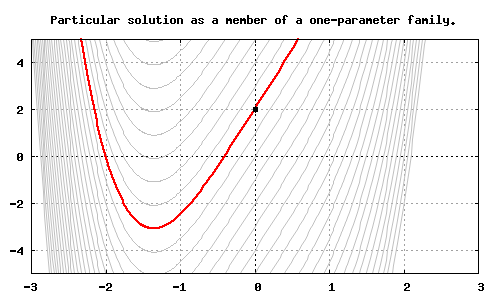
\includegraphics[width=3in]{example_4_1_1_1}

\end{exmp}

\line(1,0){60}
\linethickness{0.5mm}

\begin{exmp} Show that $y(x)=5e^{2x}$ is a particular solution of the differential equation $y'(x)=2y$.  Write down the \textit{general} solution, and use \verb|diff| to show that it works.

\begin{verbatim}
(%i8) y(x):=5*%e^(2*x)$
      diff(y(x),x);
      2*y(x);
(%o9) 10*%e^(2*x)
(%o10) 10*%e^(2*x)
\end{verbatim}

We see that $y'(x)$ and $2y$ yield exactly the same expression, so $y(x)$ satisfies the equation $y'(x)=2y$.  We notice that the factor of $2$ comes from the chain rule applied to the exponent.  The leading $5$ doesn't interfere with the differential equation at all, so we try a general solution $y(x)=c\cdot e^{2x}$.  Verifying with \verb|diff|:

\begin{verbatim}
(%i11) y(x):=c*%e^(2*x)$
       declare(c,constant)$
       diff(y(x),x);
       2*y(x);
(%o13) 2*c*%e^(2*x)
(%o14) 2*c*%e^(2*x)
\end{verbatim}

$y(x)=c\cdot e^{2x}$ is the most general function satisfying $y'(x)=2y$.


\end{exmp}

\line(1,0){60}
\linethickness{0.5mm}


\begin{exmp} Show that $y_1(x)=\sin{x}$ and $y_2(x)=\cos{x}$ are solutions of the second order ODE $y''(x)=-y$.  Explain why this ODE is linear, then show that the linear combination of solutions $c_1\cdot y_1(x)+ c_2\cdot y_2(x)$ is also a solution of the ODE.\\

\begin{verbatim}
(%i15) y_1(x):=sin(x)$
       y_2(x):=cos(x)$
       diff(y_1(x),x,2);
       diff(y_2(x),x,2);
(%o17) -sin(x)
(%o18) -cos(x)
\end{verbatim}

In each case, we see that the second derivative yields the negative of the original function, so $y_1$ and $y_2$ are both solutions. \\
${}$\\
The ODE is linear because $y$ and its derivatives appear only to the first power.  A linear combination of solutions should also be a solution:\\

\begin{verbatim}
(%i19) declare(c_1,constant,c_2,constant)$
       y_gen(x):=c_1*y_1(x)+c_2*y_2(x)$
(%i21) diff(y_gen(x),x,2);
(%o21) -c_1*sin(x)-c_2*cos(x)
\end{verbatim}

After two derivatives, we see that $y_{gen}''(x)=-y_{gen}(x)$, so the linear combination is also a solution of the ODE.   $y_{gen}(x)$ is the \textit{general} solution, since it contains two arbitrary constants.


\end{exmp}

\line(1,0){60}
\linethickness{0.5mm}


\begin{exmp} Apply the initial conditions $y(0)=0.3$ and $y'(0)=0.5$ to the general solution in Example 4.1.3.  Plot the resulting particular solution and comment on how the initial conditions relate to the graph.\\
${}$\\
Each initial condition corresponds to an equation relating $c_1$ and $c_2$.  In general, the initial conditions result in a non-trivial system of equations in $c_1$ and $c_2$, but this example is particularly simple because $\sin{x}$ vanishes at $x=0$:

\begin{verbatim}
(%i22) EQN1:y_gen(0)=0.3;
       diff(y_gen(x),x);
       EQN2:subst(0,x,%)=0.5;
(%o22) c_2=0.3
(%o23) c_1*cos(x)-c_2*sin(x)
(%o24) c_1=0.5
(%i25) y_p:sublis([c_1=0.5,c_2=0.3],y_gen(x));
(%o25) 0.5*sin(x)+0.3*cos(x)
\end{verbatim}

We see that $y_p(x)=0.5\sin{x}+0.3\cos{x}$ is the function that satisfies the original ODE and the initial conditions.  Finally, we plot the particular solution:

\begin{verbatim}
(%i26) wxdraw2d(
       grid=true,
       xrange=[-1,6],
       yrange=[-1.4,1.4],
       xaxis=true,
       yaxis=true,
       title="A particular solution of the ODE",
       color=black,
        explicit(y_p,x,-1,6)
       );
\end{verbatim}

\includegraphics[width=3in]{example_4_1_4_1}

${}$\\

Upon close inspection of the graph, we see that the initial value of the solution is about $0.3$ and the initial slope is about $0.5$, as we expect.


\end{exmp}

\line(1,0){60}
\linethickness{0.5mm}


\begin{exmp} Apply the boundary values $y(1)=-1$ and $y(3)=2$ to the general solution in Example 4.1.3.  Plot the resulting particular solution including the boundary values as points.\\

${}$\\

The boundary values result in a non-trivial system of equations this time, so we use \verb|solve| to find the values of $c_1$ and $c_2$:

\begin{verbatim}
(%i27) EQN1:y_gen(1)=-1;
       EQN2:y_gen(3)=2;
(%o27) cos(1)*c_2+sin(1)*c_1=-1
(%o28) cos(3)*c_2+sin(3)*c_1=2
(%i29) SOLUTION:solve([EQN1,EQN2],[c_1,c_2]);
(%o29) [[c_1=-(cos(3)+2*cos(1))/(sin(1)*cos(3)-cos(1)*sin(3)),
       c_2=(sin(3)+2*sin(1))/(sin(1)*cos(3)-cos(1)*sin(3))]]
\end{verbatim}

The output of \verb|solve| is a list containing a list, so we have to carefully dig out the solutions and substitute back into the general expression for $y_{gen}(x)$.  We also use \verb|float| to obtain a reasonably compact decimal approximation:

\begin{verbatim}       
(%i30) y_p:float(sublis([c_1=rhs((%[1])[1]),c_2=rhs((%[1])[2])],y_gen(x)));
(%o30) 0.099650689051389*sin(x)-2.006012470576742*cos(x)
(%i31) wxdraw2d(
       grid=true,
       xaxis=true,
       yaxis=true,
       xrange=[0,4],
       yrange=[-3,3],
       title="Particular solution from boundary values.",
       color=black,
        explicit(y_p,x,0,4),
       color=red,
       point_type=7,
        points([[1,-1],[3,2]])
       );
\end{verbatim}

\includegraphics[width=3in]{example_4_1_5_1}

\end{exmp}

\line(1,0){60}
\linethickness{0.5mm}
\pagebreak


\section{Separable Equations}\label{Separable Equations}

A first order ODE is called \textbf{separable} if we can algebraically isolate all $x$ and $y$ dependence on opposite sides of the equation.   A separable equation can be written in the form $f(y)\mathrm{d}y =g(x) \mathrm{d}x$, then we simply integrate to obtain $\displaystyle \int f(y)\ \mathrm{d}y = \displaystyle \int g(x)\ \mathrm{d}x$.  Each indefinite integral results in an arbitrary constant, but we can combine the constants into a single arbitrary constant in order to write the general solution.  The general solution might be found explicitly as a function $y(x)$, but solutions can also be defined implicitly as equations relating $y$ and $x$.


\begin{exmp} Find the general solution of $y'(x)=2y$ by separating variables.\\
${}$\\

We begin by changing to Leibniz notation:  $\displaystyle \frac{\mathrm{d}y}{\mathrm{d}x}=2y$.  Now we can obtain the form $f(y)\ \mathrm{d}y=g(x)\ \mathrm{d}x$ by dividing both sides by $y$ and multiplying both sides by $\mathrm{d}x$:  $\displaystyle \frac{\mathrm{d}y}{y}=2\ \mathrm{d}x$.  Finally, we use wxMaxima to help with the integrals:

\begin{verbatim}
(%i1) integrate(1/y,y);
      integrate(2,x);
(%o1) log(y)
(%o2) 2*x
\end{verbatim}

To set up the resulting equation, we should note that most correct answer for the $y$ integral is actually $\ln{|y|}$, and we need to insert an arbitrary constant, $c$:

\begin{verbatim}
(%i3) EQN:log(abs(y))=2*x+c;
      declare(c,constant)$
(%o4) log(abs(y))=2*x+c
(%i5) solve(EQN,y);
(%o5) [abs(y)=%e^(c+2*x)]
\end{verbatim}

The right hand side of this equation can be rewritten as $e^c e^{2x}$, but $c$ is an arbitrary constant, so we can just write $c\cdot e^{2x}$, where $c$ is a new arbitary positive constant.  In addition, $|y|=y\ \mathrm{ if }\ y>0$ and $|y|=-y\ \mathrm{ if }\ y<0$, so we can just write $y=c\cdot e^{2x}$ where $c$ is allowed to be positive or negative.  We check our general solution using \verb|diff|:

\begin{verbatim}
(%i6) y_gen:c*%e^(2*x)$
      diff(y_gen,x);
(%o7) 2*c*%e^(2*x)
\end{verbatim}

We see that $y'(x)=2y$, so we have a valid general solution.

\end{exmp}

\line(1,0){60}
\linethickness{0.5mm}

\begin{exmp} Use separation of variables to solve the ODE $y'(x)=\displaystyle \frac{\cos^2{x}}{y^3-2}$.  Find the particular solution passing through the point $[1,1]$.  Plot the family of curves in the general solution together with the particular solution shown in red.\\
${}$\\
We start by transforming to the form $(y^3-2)\ \mathrm{d}y = \cos^2{x}\ \mathrm{d}x$, then we use wxMaxima to perform the integrals.

\begin{verbatim}
(%i8) lhs:integrate(y^3-2,y);
      rhs:integrate((cos(x))^2,x);
(%o8) y^4/4-2*y
(%o9) (sin(2*x)/2+x)/2
\end{verbatim}

Now we tack on an arbitrary constant to properly express the general solution:

\begin{verbatim}
(%i10) gensolution:lhs=rhs+c;
       declare(c,constant)$
(%o10) y^4/4-2*y=(sin(2*x)/2+x)/2+c
\end{verbatim}

The general solution is defined implicitly, but we can still apply the initial condition $y=1$ when $x=1$ to find $c$ for the particular solution:

\begin{verbatim}
(%i11) sublis([x=1,y=1],gensolution);
(%o11) -7/4=(sin(2)/2+1)/2+c
(%i12) solve(%,c);
(%o12) [c=-(sin(2)+9)/4]
(%i13) partsolution:sublis([%[1]],gensolution);
(%o13) y^4/4-2*y=(sin(2*x)/2+x)/2-(sin(2)+9)/4
\end{verbatim}

Finally, we define the general solution as a function of $c$ and plot the family of curves in the general solution using \verb|makelist|.  We plot the particular solution in red.

\begin{verbatim}
(%i14) gensolution;
(%o14) y^4/4-2*y=(sin(2*x)/2+x)/2+c
(%i15) gsfunc(c):=''%;
(%o15) gsfunc(c):=y^4/4-2*y=(sin(2*x)/2+x)/2+c
(%i16) FAMILY:makelist(implicit(gsfunc(c),x,-2,2,y,-2,2),c,-10,10)$
(%i17) wxdraw2d(
       grid=true,
       dimensions=[600,600],
       xaxis=true,
       yaxis=true,
       title="curves in the general solution, and the particular solution",
       xrange=[-2,2],
       yrange=[-2,2],
       color=red,
       line_width=2,
        implicit(partsolution,x,-2,2,y,-2,2),
       color=black,
       point_type=7,
        points([[1,1]]),
       line_width=1,
       color=grey,
        FAMILY
       );
\end{verbatim}


\includegraphics[width=3in]{example_4_2_2_1}

\end{exmp}

\line(1,0){60}
\linethickness{0.5mm}
\pagebreak

\pagebreak
\section{wxMaxima's Built-In ODE Solver}\label{wxMaxima's Built-In ODE Solver}

wxMaxima can find general solutions for some first and second order ODEs using the built-in command \verb|ode2|.  We can choose to compute particular solutions manually (by solving a system of equations), or by using the built-in commands \verb|ic1| (one initial condition), \verb|ic2| (two initial conditions) or \verb|bc2| (two boundary values).  Note that many differential equations have no analytical solution.

\begin{exmp} Use \verb|ode2| to find the general solution of $y'(x)=2y$, then use \verb|ic1| to find the particular solution corresponding to the initial condition $[1,3]$. Check that the particular solution satisfies the ODE and the initial condition.  Finally, plot the particular solution together with the point $[1,3]$.\\
${}$\\
We start by solving the ODE and applying the initial conditions:

\begin{verbatim}
(%i1) eqn:'diff(y,x)=2*y;
(%o1) 'diff(y,x,1)=2*y
(%i2) sol:ode2(eqn,y,x);
(%o2) y=%c*%e^(2*x)
(%i3) ic1(sol,x=1,y=3);
(%o3) y=3*%e^(2*x-2)
\end{verbatim}

Now we check that the solution actually works:

\begin{verbatim}
(%i4) partsolution:rhs(%)$
(%i5) diff(partsolution,x);
(%o5) 6*%e^(2*x-2)
(%i6) subst(1,x,partsolution);
(%o6) 3
\end{verbatim}

We see that the first derivative gives us twice the original function, so the particular solution satisfies $y'=2y$.  The solution also satisfies the initial condition because we obtain $y=3$ when we substitute $x=1$.  Finally, we produce the plot of the particular solution:

\begin{verbatim}
(%o7) wxdraw2d(
       grid=true,
       xaxis=true,
       yaxis=true,
       xrange=[-5,5],
       yrange=[-5,5],
       title="Particular solution passing through [1,3]",
       color=black,
        explicit(partsolution,x,-5,5),
       color=red,
       point_type=7,
        points([[1,3]])
       );
\end{verbatim}


\includegraphics[width=3in]{example_4_3_1_1}

\end{exmp}

\line(1,0){60}
\linethickness{0.5mm}


\begin{exmp} Use \verb|ode2| to find the general solution of $\frac{\mathrm{d}y}{\mathrm{d}x}+xy=x^3$.  Apply the initial conditions $[1,1]$ by manually solving for the arbitrary constant, then verify that \verb|ic1| gives the same answer.

\begin{verbatim}
(%i8) eqn:'diff(y,x)+x*y=x^3;
(%o8) 'diff(y,x,1)+x*y=x^3
(%i9) sol:ode2(eqn,y,x);
(%o9) y=%e^(-x^2/2)*(((2*x^2-4)*%e^(x^2/2))/2+%c)
(%i10) sublis([x=1,y=1],%);
(%o10) 1=(%c-sqrt(%e))/sqrt(%e)
(%i11) solve(%,%c);
(%o11) [%c=2*sqrt(%e)]

(%i12) sublis(%,sol);
(%o12) y=%e^(-x^2/2)*(((2*x^2-4)*%e^(x^2/2))/2+2*sqrt(%e))

(%i13) ic1(sol,x=1,y=1);
(%o13) y=%e^(-x^2/2)*((x^2-2)*%e^(x^2/2)+2*sqrt(%e))
\end{verbatim}

The only difference between the two particular solutions is a canceled factor of 2.

\end{exmp}

\line(1,0){60}
\linethickness{0.5mm}


\begin{exmp} Find the general solution of $\frac{\mathrm{d}^2 y}{\mathrm{d} x^2}-0.3\cdot \frac{\mathrm{d}y}{\mathrm{d}x}-2y=0$ using \verb|ode2|, then apply the initial conditions $y(0)=1.2$ and $y'(0)=0.4$ using \verb|ic2|.  Verify that your particular solution solves the original ODE.

\begin{verbatim}
(%i14) ratprint:false$
(%i15) eqn:'diff(y,x,2)-0.3*'diff(y,x)-2*y=0;
(%o15) 'diff(y,x,2)-0.3*('diff(y,x,1))-2*y=0
(%i16) gensolution:ode2(eqn,y,x);
(%o16) y=%k1*%e^(((sqrt(809)/10+3/10)*x)/2)
        +%k2*%e^(((3/10-sqrt(809)/10)*x)/2)
(%i17) partsolution:rhs(ic2(gensolution,x=0,y=1.2,'diff(y,x)=0.4));
(%o17) ((11*sqrt(809)+2427)*%e^(((sqrt(809)/10+3/10)*x)/2))/4045
      -((11*sqrt(809)-2427)*%e^(((3/10-sqrt(809)/10)*x)/2))/4045
\end{verbatim}

Now we check our particular solution by substituting it for $y$ in the original differential equation:

\begin{verbatim}
(%i18) fullratsimp(diff(partsolution,x,2)-0.3*diff(partsolution,x)
      -2*partsolution);
(%o18) 0
\end{verbatim}


\end{exmp}

\line(1,0){60}
\linethickness{0.5mm}

\begin{exmp} Find the solution of $\frac{\mathrm{d}^2 y}{\mathrm{d}x^2}=-9\cdot y(x)$ subject to the boundary conditions $y(0)=0$ and $y(5)=2$.  Make a plot to verify that the boundary conditions are satisfied.\\

${}$\\

We find the general solution, then use \verb|bc2| to apply the boundary conditions:

\begin{verbatim}
(%i19) eqn:'diff(y,x,2)=-9*y;
(%o19) 'diff(y,x,2)=-9*y
(%i20) gensoln:ode2(eqn,y,x);
(%o20) y=%k1*sin(3*x)+%k2*cos(3*x)
(%i21) bc2(gensoln,x=0,y=0,x=5,y=2);
(%o21) y=(2*sin(3*x))/sin(15)
\end{verbatim}

Now we produce the plot:

\begin{verbatim}
(%i22) partsolution:rhs(%);
(%o22) (2*sin(3*x))/sin(15)
(%i23) wxdraw2d(
       grid=true,
       xaxis=true,
       yaxis=true,
       xrange=[-.5,5.5],
       yrange=[-4,4],
       title="A particular solution satisfying two boundary values.",
       color=black,
        explicit(partsolution,x,0,5),
       color=red,
       point_type=7,
        points([[0,0],[5,2]])
       );
\end{verbatim}

\includegraphics[width=3in]{example_4_3_4_1}

\end{exmp}

\line(1,0){60}
\linethickness{0.5mm}
\pagebreak

\pagebreak

\section{Direction Fields}\label{Direction Fields}

Direction fields are a graphical tool for understanding the solutions of first order equations of the form $\frac{\mathrm{d}y}{\mathrm{d}x}=f(x,y)$.  For an equation of this form, we immediately know the \textit{slope} of $y(x)$ at any point $(x,y)$ by simply plugging $x$ and $y$ into the right hand side.  A direction field (also called a slope field) is constructed by computing the slope at many points in the plane.  Once an initial condition is specified, the particular solution simply follows the ``flow'' of the direction field.  wxMaxima has a built-in command \verb|wxdrawdf| creating a direction field (with or without a particular solution).

\begin{exmp} Plot a direction field for the ODE $y'(x)=2y$, then produce a plot showing the particular solution passing through $[1,3]$.\\
${}$\\
First, we plot the direction field with no particular solution:

\begin{verbatim}

(%i1) load(drawdf)$
(%i2) wxdrawdf(2*y,[x,-10,10],[y,-10,10]);
\end{verbatim}

Any particular solution will follow the ``flow'' of this field (the slope of any solution matches the slope of the line segments at any point).  Now we add the particular solution to the direction field:

\begin{verbatim}
(%i3) wxdrawdf(2*y,[x,-10,10],[y,-10,10],[trajectory_at,1,3]);
\end{verbatim}


\includegraphics[width=3in]{example_4_4_1_1}
\includegraphics[width=3in]{example_4_4_1_2}
\end{exmp}

\line(1,0){60}
\linethickness{0.5mm}
\pagebreak

\begin{exmp} Plot a direction field for the ODE $y'(x)=y(1-y)$.  Comment on the intervals of initial conditions (at $x=0$) that produce distinctly different types of particular solutions.  In addition, there are two initial conditions that produce constant particular solutions (\textit{equilibrium} solutions).  Plot an example of each type of particular solution in addition to the equilibrium solutions.\\
${}$\\
We plot the direction field using \verb|wxdrawdf|:

\begin{verbatim}
(%i4) wxdrawdf(y*(1-y),[x,-.5,5],[y,-1,2]);
\end{verbatim}

\includegraphics[width=3in]{example_4_4_2_1}

We see that particular solutions will behave differently on the $y$-intervals $(-\infty,0)$ (these solutions run away to $-\infty$), $(0,1)$ (these solutions approach $y=1$ from below) and $(1,\infty)$ (these solutions approach $y=1$ from above). Initial conditions at $(0,0)$ and $(1,1)$ result in \textit{constant} particular solutions.  We plot particular solutions corresponding to the initial conditions $y(0)=-0.5$, $y(0)=0$, $y(0)=0.5$, $y(0)=1$ and $y(0)=1.5$:

\begin{verbatim}
(%i5) wxdrawdf(y*(1-y),[x,-.5,5],[y,-1,2],[trajectory_at,0,-0.5],
      [trajectory_at,0,0],[trajectory_at,0,0.5],[trajectory_at,0,1],
      [trajectory_at,0,1.5]);
\end{verbatim}

\includegraphics[width=3in]{example_4_4_2_2}

\end{exmp}

\line(1,0){60}
\linethickness{0.5mm}
\pagebreak

\section{Euler's Method}\label{Euler's Method}

Euler's Method is a numerical method for approximating a particular solution to a first order ODE of the form $\frac{\mathrm{d}y}{\mathrm{d}x}=f(x,y)$.  To approximate a solution with initial condition $(x_0,y_0)$, we use the ODE to find the slope $y_0'$ at $(x_0,y_0)$, then we take a small step $\Delta x$ to the right, using the slope to approximate the next $y$ value:  $x_1=x_0+\Delta x$, and $y_1=y_0+y_0'\cdot \Delta x$.  This process is repeated until we obtain the desired approximation to the particular solution -- either $y(c)$ for some particular location, or possibly $y(x)$ for an entire interval.  The approximation becomes more accurate as the step size $\Delta x$ becomes smaller.  \\
${}$\\
Euler's method uses the output of each step as the input for the next step, so a looping structure is clearly appropriate.  We use a \verb|for-do| loop to generate a list of coordinates (starting with the initial condition) until the desired approximation is obtained.

\begin{exmp} Use Euler's method to approximate $y(2)$ for the ODE $y'(x)=2y$ with initial condition $(1,3)$.  Perform approximations by breaking the interval $(1,2)$ into $n=2,5,10$ pieces.  Compare to wxMaxima's \verb|ode2| solution.  Finally, use a large enough $n$ to obtain an Euler approximation accurate to two decimal places.\\
${}$\\
We define the differential equation, the starting point $(x_0,y_0)=(X,Y)$, and $\Delta x =\frac{(2-1)}{n}$, then we set up the loop to compute the next $x$ and $y$ values at each step:  $x_{i+1}=x_i+\Delta x$ and $y_{i+1}= y_i+y_i'\cdot \Delta x$.  We run the loop for $n=2,5,10$ (only the $n=2$ case is shown below).  The outputs of all three approximations are shown side-by-side below:

 
\begin{verbatim}

(%i1) DIFF(y):=2*y$
      delx(n):=(2-1)/n$
(%i3) X:1$
      Y:3$
      n:2$
(%i6) (print(" x ....... y"),
       print(float(X),"......",float(Y)),
       for k:1 thru n do
       (SLOPE:DIFF(Y),
        NEXTY:Y+SLOPE*delx(n),
        NEXTX:X+delx(n),
        print(float(NEXTX),"......",float(NEXTY)),
        Y:NEXTY,
        X:NEXTX)
      );

\end{verbatim}
\pagebreak
\begin{verbatim} 
  
 x .......y       x .......y             x .......y  
1.0......3.0     1.0......3.0           1.0......3.0
1.5......6.0     1.2......4.2           1.1......3.6
2.0......12.0    1.4......5.88          1.2......4.32
                 1.6......8.231999      1.3......5.184
                 1.8......11.5248       1.4......6.2208
                 2.0......16.13472      1.5......7.46496
                                        1.6......8.957952
                                        1.7......10.749542
                                        1.8......12.899450
                                        1.9......15.479341
                                        2.0......18.575209

\end{verbatim}

We obtain approximations of $y(2)\approx 12.0$ ($n=2$), $y(2)\approx 16.1$ ($n=5$) and $y(2)\approx 18.6$ ($n=10$).\\
${}$\\
Finally, we compute the \verb|ode2| approximation:

\begin{verbatim}
(%i7) EQN:'diff(y,x)=2*y$
      SOLN:ode2(EQN,y,x);
(%o8) y=%c*%e^(2*x)
(%i9) PARTSOLN:ic1(SOLN,x=1,y=3);
(%o9) y=3*%e^(2*x-2)
(%i10) float(subst(2,x,PARTSOLN));
(%o10) y=22.16716829679195
\end{verbatim}

With $y(2)\approx 22.2$, we see that the $n=2,n=5$ and $n=10$ Euler approximations are not very accurate (though they are getting closer to the right answer as $n$ increases).  We can improve the approximation by simply increasing $n$.  We modify the do-loop with an \verb|if-else| statement to print only the final step for an approximation of $y(2)$, and we use $n=9999$:

\begin{verbatim}
(%i11) kill(all)$
(%i1) DIFF(y):=2*y$
      delx(n):=(2-1)/n$
(%i3) X:1$
      Y:3$
      n:9999$
(%i6) (for k:1 thru n do
       (SLOPE:DIFF(Y),
        NEXTY:Y+SLOPE*delx(n),
        NEXTX:X+delx(n),
        if(k=n) then print("y(2)=",float(NEXTY)),
        Y:NEXTY,
        X:NEXTX)
      );
      
y(2)=22.1627354541832
(%o6) done
\end{verbatim}

The $n=9999$ approximation agrees to two decimal places, but it takes an average computer a very long time to compute.  Euler's method is a relatively weak approximation scheme, but it's instructive nonetheless.

\end{exmp}

\line(1,0){60}
\linethickness{0.5mm}

\begin{exmp} Use Euler's method to plot an approximate solution to $y'(x)=xy\sin{y}$ on $(0,5)$ for the initial condition $(0,1.5)$.  Apply the approximation using $n=2$, $n=10$, $n=20$ and $n=100$.\\
${}$\\
To plot results from a do-loop, we use \verb|append| to tack on a new point to a list of points with each iteration.  The code is shown below only for $n=2$, but all four approximations are plotted.  Note that we use \verb|float| to obtain decimal approximations for the points in order to reduce the demands on our machine (without this improvement in the code, wxMaxima ``hangs'' on the $n=100$ case):

\begin{verbatim}
(%i7) kill(all)$
      DIFF(x,y):=x*y*sin(x)$
      delx(n):=(5-0)/n$
      X:0$
      Y:1.5$
      n:2$
      POINTS:[[X,Y]]$
      
(%i8) (for k:1 thru n do
      (SLOPE:DIFF(X,Y),
       NEXTY:float(Y+SLOPE*delx(n)),
       NEXTX:float(X+delx(n)),
       POINTS: append(POINTS,[[NEXTX,NEXTY]]),
       Y:NEXTY,
       X:NEXTX)
       );
(%o8) done

(%i10) wxdraw2d(
       xrange=[-0.1,5.1],
       yrange=[-40,40],
       title="n=2 Euler approximation",
       points_joined=true,
       color=black,
       points(POINTS)
       );
\end{verbatim}

\includegraphics[width=2.7in]{example_4_5_2_1}
\includegraphics[width=2.7in]{example_4_5_2_2}

\includegraphics[width=2.7in]{example_4_5_2_3}
\includegraphics[width=2.7in]{example_4_5_2_4}

As a check on our approximation, we use \verb|wxdrawdf| to view the particular solution within a direction field:

\begin{verbatim}
(%i11) load(drawdf)$
(%i12) wxdrawdf(x*y*sin(x),[x,-.5,5.1],[y,-40,40],[trajectory_at,0,1.5]);
\end{verbatim}

\includegraphics[width=3in]{example_4_5_2_5}

\end{exmp}

\line(1,0){60}
\linethickness{0.5mm}
\pagebreak

\section{Module 4 Exercises}\label{Module 4 Exercises}

\begin{enumerate}

\item  Show that $y(x)=c\cdot e^{x^2/2} +3$ is the general solution of the ODE $\frac{\mathrm{d}y}{\mathrm{d}x}=xy-3x$.  Use \verb|makelist| to generate 20 members of the family of solutions satisfying the ODE.  Plot the family of solutions in grey together with the particular solution satisfying $y(0)=5$ in red.

\item  Show that $y_1(x)=\sin{(\omega x)}$ and $y_2(x)=\cos{(\omega x)}$ are both solutions of the second order ODE $y''(x)=-\omega^2 y(x)$ (use \verb|%omega| in wxMaxima).  What is the general solution for the ODE?  Show that $y(x)=A\cdot \cos(\omega x+\phi)$ is an alternative general solution (with arbitrary constants $A$ and $\phi$).  

\item  Find the particular solution of $y''(x)=-5 y(x)$ subject to the boundary values $y(0)=2$ and $y(3.1)=-0.2$.  Rather than using \verb|bc2|, use \verb|subst| and \verb|solve| to ``manually'' find the particular solution in two different forms using the different expressions of the general solution discussed in the previous Exercise. Use \verb|trigexpand| to show that the two particular solutions are equivalent.  Finally, plot the particular solution including the points given by the boundary values. 

\item  Show that $c_1 e^{kx}+c_2 e^{-kx}$ is the general solution of $y''(x)=k^2\cdot y(x)$.  The general solution looks very much like a pair of ``special'' functions -- what are they?  Show that each of these special functions also satisfies the ODE, then write down the general solution in terms of these functions.

\item  Use separation of variables to find the general solution of $y'(x)=-y/x$.  Make a plot of the family of curves in the general solution by using \verb|makelist|.

\item  Use separation of variables to find the general solution of $y'(x)=+y/x$.  Make a plot of the family of curves in the general solution by using \verb|makelist|.

\item  Use separation of variables to find the particular solution of $\frac{\mathrm{d}y}{\mathrm{d}x}=\frac{x^2 \sqrt{x^2+3}}{(1-y^2)^{3/2}}$ subject to the initial condition $y(3)=0.5$.  Plot the particular solution, showing that it passes through $(3,0.5)$.

\item  Use \verb|ode2| to find the general solution of $y'(x)=-\frac{1}{2}y\cdot \tan{x}$.  Plot the family of solutions for 20 values of \verb|%c| in the general solution.

\item  Use \verb|ode2| to find the general solution of $y'(x)=-\sin{y}\cdot \cos{x}$.  Plot the family of solutions for 20 values of \verb|%c| in the general solution.

\item  Plot a direction field for the ODE $y'(x)=\frac{\sin^2{x}}{y}$, including a plot of the particular solution passing through $(0,1)$.

\item  Use Euler's method with $n=100$ to plot the particular solution in the previous exercise on $[0,5]$.

\item  Plot the direction field for $y'(x)=-\frac{x}{y}$, including particular solutions passing through $(0,1)$, $(0,2)$ and $(0,3)$.  

\item  For the ODE in the previous exercise, use Euler's method with $n=100$ to plot the particular solution passing through $(0,3)$.


\item  A classic problem in differential equations is to find a set of \textit{orthogonal trajectories} to a given family of curves.  The orthogonal trajectories are curves that intersect the given family at right angles at every point.  Consider the family of curves $y=-\frac{C}{x}$.  To find its orthogonal trajectories, we must first find the slope at any point, for any value of $C$; that is, we compute $\frac{\mathrm{d}y}{\mathrm{d}x}$ in terms of $C$.  In this case, the derivative is trivial:  $\frac{\mathrm{d}y}{\mathrm{d}x} = \frac{C}{x^2}$.\\
${}$\\
To intersect at right angles, the orthogonal set must have the negative reciprocal of slope at each point.  In other words, the orthogonal trajectories satisfy a differential equation $\frac{\mathrm{d}y}{\mathrm{d}x}= -\frac{x^2}{C}$ (note that $C=0$ must be excluded at this point).  To solve this differential equation, substitute the expression for $C$ in terms of $x$ and $y$, then separate variables and integrate (alternatively, you can use \verb|ode2|). You will obtain a new family of curves (with a new arbitrary constant $D$) that should intersect the original family at right angles.  Finally, use \verb|makelist| to generate plots of the two families of curves for $C=-10,-9,\dots 10$ (excluding $C=0$) and $D=-10,-9,\dots 10$

\item  \textit{Logistic growth} occurs when a population grows nearly exponentially when it is small, then levels off to a ``carrying capacity'' when it becomes sufficiently large.  The model for logistic growth is a differential equation $\frac{\mathrm{d}N}{\mathrm{d}t}=kN\cdot (L-N)$, where $N$ is the population size, and $L$ is the carrying capacity.  We can determine by inspection that the growth is nearly exponential when $N$ is small:   $\frac{\mathrm{d}N}{\mathrm{d}t}\approx (kL)N$, and the growth rate approaches zero as $N\to L$.  Additionally, we see that the growth rate becomes negative if $N>L$; in other words, the population will become smaller if it exceeds the carrying capacity of the environment.  \\
${}$\\
Suppose that a rabbit population grows logistically with $k=0.312$ and $L=1000$.  Assume that the time units are weeks.

 \begin{enumerate}
 
  \item Plot the population as a function of time using the initial conditions $N(0)=2$ and $N(0)=5$.  

  \item How long does it take each population to reach 80\verb|%| of the carrying capacity?
  
  \item Suppose the rabbits have an overpopulation problem:  $N(0)=2000$.  Plot the population as a function of time.  How long does it take before the population shrinks to 1200 rabbits?
  
  \item Determine how the population behaves if $N(0)=1000$.
 \end{enumerate}
 
\item  \textit{Radioactive decay} is governed by probabilistic physics -- each atom of an unstable isotope carries exactly the same probability of decay per second.  For example, if an isotope has a decay probability of $k=.001$ per atom per second, and we have a collection of 2000 atoms, we expect 2 decays in the next second.  This behavior can be modeled with a first order differential equation:  $\frac{\mathrm{d}N}{\mathrm{d}t}=-kN$; that is, the decay rate (atoms per second) is proportional to the number of atoms.  The solution to this ODE is guessable -- write it down, making sure to properly include an arbitrary constant.  Now plug in $t=0$, and interpret the arbitrary constant.  \\
${}$\\
Carbon-14 atoms have a probability of decay per atom per \textit{year} of about $k\approx .000121$.  

 \begin{enumerate}

  \item Starting with $N(0)=10^{23}$, produce a plot of $N(t)$ for a period of 20,000 years.  
  
  \item Compute the percent of original atoms remaining after 10,000 years.  
  
  \item Compute the time for half the atoms to decay (this is called the half-life for Carbon-14).

 \end{enumerate}
 
 Note:  C-14 is used in \textit{radiometric dating} of archaeological remains.  The actual technique requires knowledge of the \textit{percent} of carbon in the form of C-14 at the time of an organism's death.  This percent is relatively stable over time, as C-14 is produced by a predictable process in the Earth's upper atmosphere.  When an organism is alive, it incorporates carbon from its environment, including this same fraction of C-14.  When an organism dies, the fraction of C-14 decreases as C-14 decays to N-14, while the ``ordinary'' carbon C-12 is stable.  The \textit{fraction} of C-14 follows the same decay curve as the \textit{amount} of C-14 to a very good approximation because C-14 only occurs in trace amounts (about one part per trillion).  

\item If the acceleration of an object is constant, we can describe its behavior with a second order differential equation, $x''(t)=a$, where $a$ is the constant acceleration. Solve this ODE with the initial conditions $x(0)=x_0$ and $v(0)=v_0$ to obtain the standard constant-acceleration equations of motion $x(t)$ and $v(t)$.

\item Find the equations of motion for an object with acceleration $a(t)=te^{-t}$.  Use the standard initial conditions from the previous Exercise.


\end{enumerate}

\pagebreak


\chapter{Parametric and Polar Curves}

\vspace*{\fill}

\minitoc

\vspace*{\fill}


\flushleft{\textbf{\Large Key Commands Included in This Module}}
\newline
\newline

\begin{tabular}{l l l}
 \verb|makelist   |   &\verb|trigsimp   |   &\verb|integrate   |   \\
 \verb|parametric   |   &\verb|diff   |   &\verb|quad_qag   |   \\
 \verb|eliminate   |   &\verb|float   |   &\verb|polar   |   \\
 \verb|solve   |   &\verb|find_root   |   &\verb|subst   |   \\
 \verb|dimensions   |   &\verb|ratprint:false   |   &\verb|   |   \\
\end{tabular}



\pagebreak
\section{Parametric Equations}\label{Parametric Equations}

We define a curve \textit{parametrically} by specifying the $x$ and $y$ coordinates individually as functions of a parameter, usually $t$.  The \textbf{parametric equations} of the curve are 
\[x(t)=f(t)\ \mathrm{ and }\ y(t)=g(t)\]
When we choose a particular value of $t$, an ordered pair $(x,y)$ is determined by the equations.  If we evaluate the equations for a range of $t$ values on the interval $[a,b]$, the result is a curve in the plane starting at $(x(a),y(a))$ and ending at $(x(b),y(b))$.  The curve has \textit{direction} corresponding to the order in which the points are plotted as $t$ increases.\\
${}$\\
It is often possible to algebraically combine the parametric equations into a single equation relating only $x$ and $y$.  This process can occasionally give us more insight into the curve, but the directionality is lost in the process. 

${}$\\

\begin{exmp}  Evaluate the parametric equations $x(t)=t$ and $y(t)=2t-3$ at $t=0,0.1,0.2,\dots 2$.  Make a plot showing the discrete points together with the continuous parametric curve traced out for the $t$ interval $[-1,3]$.  Finally, algebraically combine the parametric equations to obtain an equation relating only $x$ and $y$, and verify that this equation agrees with the plot. \\
${}$\\

We define the parametric equations for $x$ and $y$, then use \verb|makelist| to make the set of discrete points.  Finally we produce the plot including the continuous parametric curve:

\begin{verbatim}
(%i1) x(t):=t$
      y(t):=2*t-3$
      
(%i3) POINTS:makelist([x(0.1*n),y(0.1*n)],n,0,20);
(%o3) [[0,-3],[0.1,-2.8],[0.2,-2.6],[0.3,-2.4],[0.4,-2.2],
      [0.5,-2.0],[0.6,-1.8],[0.7,-1.6],[0.8,-1.4],[0.9,-1.2],
      [1.0,-1.0],[1.1,-0.8],[1.2,-0.6],[1.3,-0.4],[1.4,-0.2],
      [1.5,0.0],[1.6,0.2],[1.7,0.4],[1.8,0.6],[1.9,0.8],[2.0,1.0]]
      
(%i4) wxdraw2d(
      grid=true,
      xaxis=true,
      yaxis=true,
      title="Points on a parametric curve.",
      color=dark_grey,
       parametric(x(t),y(t),t,-1,3),
      color=red,
      point_type=7,
       points(POINTS)
      );
\end{verbatim}

\includegraphics[width=3in]{example_5_1_1_1}

The implicit directionality of this plot points in the direction of increasing $t$.  We see from the list of discrete points that the directionality is ``up and to the right'' along the curve.  Finally, we algebraically ``eliminate the parameter'' to obtain an equation relating only $x$ and $y$. We redefine the parametric functions as \textit{equations} in wxMaxima, then we apply \verb|eliminate| to the system to eliminate $t$. Note that the output of \verb|eliminate| is implicitly set equal to zero -- we use \verb|solve| to state the resulting equation in a more standard form.

\begin{verbatim}
(%i5) Xeqn:x=x(t)$
      Yeqn:y=y(t)$
      eliminate([Xeqn,Yeqn],[t]);
(%o7) [-y+2*x-3]
(%i8) solve(%[1]=0,y);
(%o8) [y=2*x-3]
\end{verbatim}

We obtain the equation of a line with slope 2 and $y$-intercept -3, as we observe in the plot.

\end{exmp}

\line(1,0){60}
\linethickness{0.5mm}


\begin{exmp} Plot the parametric curve defined by $x(t)=3\cos{t}$ and $y(t)=3\sin{t}$ on the $t$-interval $[0,2\pi]$.  Explicitly label the points at $t=0,\frac{\pi}{2},{\pi}, \frac{3\pi}{2}$ and comment on the directionality of the curve.  Finally, express the equation of the curve entirely in terms of $x$ and $y$.\\


\begin{verbatim}
(%i9) x(t):=3*cos(t)$
      y(t):=3*sin(t)$
(%i11) wxdraw2d(
       grid=true,
       xaxis=true,
       yaxis=true,
       xrange=[-4,4],
       yrange=[-4,4],
       dimensions=[600,600],
       nticks=600,
       color=black,
        parametric(x(t),y(t),t,0,2*%pi),
       color=red,
       point_type=7,
        points([[x(0),y(0)],[x(%pi/2),y(%pi/2)],[x(%pi),y(%pi)],[x(3*%pi/2),y(3*%pi/2)]]),
       color=black,
        label(["t=0",3.5,0]),
        label(["t=pi/2",0,3.3]),
        label(["t=pi",-3.5,0]),
        label(["t=3pi/2",0,-3.3])
       );
\end{verbatim}

\includegraphics[width=3in]{example_5_1_2_1}

We see that the direction of increasing $t$ is counterclockwise.  Finally, we eliminate the parameter to obtain a familiar equation for this curve.  Note that \verb|eliminate| won't work in this case, because it is designed only for polynomial equations.  We proceed by exploiting a trig identity:

\begin{verbatim}
(%i12) Xeqn:x=x(t);
       Yeqn:y=y(t);
(%o12) x=3*cos(t)
(%o13) y=3*sin(t)
(%i14) Xeqn^2+Yeqn^2;
(%o14) y^2+x^2=9*sin(t)^2+9*cos(t)^2
(%i15) trigsimp(%);
(%o15) y^2+x^2=9
\end{verbatim}

We recognize the equation of a circle of radius 3 centered at the origin.

\end{exmp}

\line(1,0){60}
\linethickness{0.5mm}

\begin{exmp} Plot the parametric curve defined by $x(t)=\cos(7t)$ and $y(t)=\sin(3t)$.  Choose a $t$ interval sufficiently large to close the curve.\\

${}$\\

As $t$ goes from $0$ to $2\pi$, $x(t)$ completes 7 periods and $y(t)$ completes 3 periods.  At $t=2\pi$, the coordinates reach their original starting point, so we only need to plot the curve on $[0,2\pi]$ to get the whole picture.  This type of curve is known as a Lissajous figure:

\begin{verbatim}
(%i21) wxdraw2d(
       grid=true,
       xaxis=true,
       yaxis=true,
       title="A Lissajous curve.",
       color=black,
       nticks=600,
       dimensions=[600,600],
        parametric(cos(7*t),sin(3*t),t,0,2*%pi)
       );
\end{verbatim}

\includegraphics[width=3in]{example_5_1_3_1}

${}$\\
In the Exercises, we use an animation to explore the directionality of this curve.

\end{exmp}

\line(1,0){60}
\linethickness{0.5mm}
\pagebreak


\pagebreak
\section{Calculus Applications for Parametric Curves}\label{Calculus Applications for Parametric Curves}

\subsection{Slope of a Parametric Curve}

When a curve is defined parametrically, we can find the slope, $\frac{\mathrm{d}y}{\mathrm{d}x}$ at $t=a$ by using the $t$-derivatives of $x$ and $y$:\\
\[\frac{\mathrm{d}y}{\mathrm{d}x}=\frac{\mathrm{d}y / \mathrm{d}t}{\mathrm{d}x / \mathrm{d}t}=\frac{y'(a)}{x'(a)}\]
${}$\\
We can use the the slope to plot a tangent line to a parametric curve at any desired point.

\begin{exmp} A parametric curve is defined by $x(t)=t\sin{t}$ and $y(t)=t-3$ on the $t$-interval $[0,2\pi]$.  Compute the slope and the equation of the tangent line at $t=2.5$ and plot the curve together with the tangent line.\\
${}$\\

We define the slope as a ratio of $y'(t)$ and $x'(t)$, compute the slope at $t=2.5$, and compute the equation of the tangent line by plugging $(x(2.5),y(2.5))$ into the point-slope formula.  We use \verb|float| to obtain decimal approximations because \verb|wxdraw2d| struggles with the exact expressions:

\begin{verbatim}
(%i1) x(t):=t*sin(t)$
      y(t):=t-3$
      
(%i3) diff(x(t),t);
(%o3) sin(t)+t*cos(t)
(%i4) x_prime(t):=''(%);
(%o4) x_prime(t):=sin(t)+t*cos(t)
(%i5) diff(y(t),t);
(%o5) 1
(%i6) y_prime(t):=''(%);
(%o6) y_prime(t):=1

(%i7) y_prime(t)/x_prime(t);
(%o7) 1/(sin(t)+t*cos(t))
(%i8) SLOPE(t):=''(%);
(%o8) SLOPE(t):=1/(sin(t)+t*cos(t))

(%i9) slope:float(SLOPE(2.5));
(%o9) -0.71205449419157
(%i10) tanline:float(slope*(x-x(2.5))+y(2.5));
(%o10) -0.71205449419157*(x-1.496180360259891)-0.5

(%i11) wxdraw2d(
       grid=true,
       xaxis=true,
       yaxis=true,
       xrange=[-5,5],
       yrange=[-5,5],
       title="A parametric curve with a tangent line.",
       color=dark_grey,
        parametric(x(t),y(t),t,0,2*%pi),
       color=red,
        explicit(tanline,x,-5,15),
       color=black,
       point_type=7,
        points([[x(2.5),y(2.5)]]),
        label(["(x(2.5),y(2.5))",2,.5])
       );
\end{verbatim}

\includegraphics[width=3in]{example_5_2_1_1}

\end{exmp}

\line(1,0){60}
\linethickness{0.5mm}


\begin{exmp} The equations $x(t)=t-1.5\sin{t}$ and $y(t)=1-1.5\cos{t}$ define a \textit{prolate cycloid}.  For the $t$ interval $[1,10]$, find all the values of $t$ for which a tangent line has zero slope or undefined slope.  Finally, plot the prolate cycloid together with the tangent lines.\\

${}$\\

We compute the slope as a function of $t$ and make a preliminary sketch of the curve to aid our search for the relevant points:

\begin{verbatim}
(%i1) x(t):=t-1.5*sin(t)$
      y(t):=1-1.5*cos(t)$
      diff(x(t),t)$
      x_prime(t):=''(%);
      diff(y(t),t)$
      y_prime(t):=''(%);
(%o4) x_prime(t):=1-1.5*cos(t)
(%o6) y_prime(t):=1.5*sin(t)

(%i7) y_prime(t)/x_prime(t)$
      SLOPE(t):=''(%);
(%o8) SLOPE(t):=(1.5*sin(t))/(1-1.5*cos(t))

(%i9) wxdraw2d(
      grid=true,
      xaxis=true,
      yaxis=true,
      title="Sketch of a prolate cycloid.",
      color=black,
       parametric(x(t),y(t),t,1,10)
      );
\end{verbatim}

\includegraphics[width=3in]{example_5_2_2_1}

Now we locate the values of $t$ for which the numerator and denominator of \verb|SLOPE| vanish.  The numerator, $1.5\sin{t}$ vanishes at $t=\pi$, $t=2\pi$ and $t=3\pi$.  We use \verb|find_root| to locate the values of $t$ for which the denominator vanishes.  The vertical tangents occur just before and after $t=2\pi$ (the location of the horizontal tangent) so we use the intervals $[4,2\pi]$ and $[2\pi,8]$:

\begin{verbatim}
(%i10) find_root(denom(SLOPE(t)),t,4,2*%pi);
(%o10) 5.442116636611656

(%i11) find_root(denom(SLOPE(t)),t,2*%pi,8);
(%o11) 7.124253977747517
\end{verbatim}

We have vertical tangents at $t\approx 5.44$ and $t\approx 7.12$.  Finally, we produce a plot of the prolate cycloid together with the tangent lines (recall that the vertical tangent lines must be defined parametrically):

\begin{verbatim}
(%i12) wxdraw2d(
       grid=true,
       xaxis=true,
       yaxis=true,
       yrange=[-2,3],
       xrange=[-1,11],
       title="Prolate cycloid with horizontal and vertical tangents.",
       color=dark_grey,
       line_width=2,
        parametric(x(t),y(t),t,1,10),
       line_width=1,
       line_type=dots,
       color=red,
        explicit(y(%pi),x,-1,11),
        explicit(y(2*%pi),x,-1,11),
        explicit(y(3*%pi),x,-1,11),
        parametric(x(5.442),t,t,-2,3),
        parametric(x(7.124),t,t,-2,3)
        );
\end{verbatim}


\includegraphics[width=3in]{example_5_2_2_2}


\end{exmp}

\line(1,0){60}
\linethickness{0.5mm}


\subsection{Arc Length of a Parametric Curve}

We approach the arc length problem by visualizing a small element of arc on the curve defined by the parametric equations $x(t)$ and $y(t)$:

${}$\\

\includegraphics[width=2.7in]{figure_5_2_2_1} %zoomed out
\includegraphics[width=2.7in]{figure_5_2_2_2} %zoomed in

When we zoom in on $\mathrm{d}s$, we see that it can be decomposed into $x$ and $y$ components, and we apply the pythagorean theorem to obtain $ \mathrm{d}s= \sqrt{(\mathrm{d}x)^2+(\mathrm{d}y)^2}$. This time, we proceed by factoring $\mathrm{d}t$ out of the square root to obtain $\mathrm{d}s= \sqrt{\left( \frac{\mathrm{d}x}{\mathrm{d}t}\right)^2+\left( \frac{\mathrm{d}y}{\mathrm{d}t}\right) ^2}\ \mathrm{d}t$. \\
${}$\\

Finally, we set up arc length as an integral for the $t$-interval $[a,b]$:

\[S=\int \mathrm{d}s = \int_a^b \sqrt{(x'(t))^2+(y'(t))^2}\ \mathrm{d}t\]

${}$\\

\begin{exmp} Compute the arc length of the ellipse defined by the parametric equations $x(t)=3\cos{t}$ and $y(t)=1.5\sin{t}$ on the $t$-interval $[0,2\pi]$.\\

${}$\\

We define $x(t)$ and $y(t)$, apply \verb|diff| and attempt the integral:

\begin{verbatim}
(%i13) x(t):=3*cos(t)$
       y(t):=1.5*sin(t)$
         
(%i15) diff(x(t),t)$
       x_prime:%;      
(%o16) -3*sin(t)

(%i17) diff(y(t),t)$
       y_prime:%;
(%o18) 1.5*cos(t)

(%i19) ratprint:false$

(%i20) integrate(sqrt(x_prime^2+y_prime^2),t,0,2*%pi);
\end{verbatim}

\verb|(%o20)  | $\displaystyle \int_{0}^{2\,\pi }\sqrt{9\,{\mathrm{sin}\left( t\right) }^{2}+2.25\,{\mathrm{cos}\left( t\right) }^{2}}dt$\\

${}$\\

wxMaxima fails to compute the integral, so we use \verb|quad_qag| instead.  

\begin{verbatim}
(%i21) quad_qag(sqrt(x_prime^2+y_prime^2),t,0,2*%pi,1);
(%o21) [14.53267233082058,1.0286549418261626*10^-7,165,0]
\end{verbatim}

We obtain an arc length of $S\approx 14.5$.  Finally, we produce a plot of the ellipse to make sure our answer is reasonable:

\begin{verbatim}
(%i22) wxdraw2d(
       grid=true,
       xaxis=true,
       yaxis=true,
       title="ellipse with arc length ~14.5",
       color=black,
        parametric(x(t),y(t),t,0,2*%pi)
       );
\end{verbatim}

\includegraphics[width=3in]{example_5_2_3_1}

\end{exmp}

\line(1,0){60}
\linethickness{0.5mm}
\pagebreak

\section{Polar Coordinates}\label{Polar Coordinates}

\subsection{Polar Coordinates and Coordinate Transformations}

To define a point in polar coordinates, we specify a distance from the origin, $r$, and a direction, $\theta$ (measured in radians counterclockwise from the positive $x$ axis).  The point is then given by an ordered pair $(r,\theta)$.  We can specify a point in polar coordinates in an infinte number of ways by tacking on multiples of $2\pi$ to $\theta$, and we can even use negative values of $r$ or $\theta$. \\
${}$\\
We can transform between polar and rectangular coordinates using trigonometry:\\
${}$\\

\verb|        |Polar to Rectangular: \verb|     | $x=r\cdot \cos{\theta}$ \verb|     | $y=r\cdot \sin{\theta}$\\
${}$\\
\verb|        |Rectangular to Polar: \verb|     | $r=\sqrt{x^2+y^2}$ \verb|   |  $\theta = \tan^{-1} \frac{y}{x}$

${}$\\
Note that the inverse tangent only yields values of $\theta$ on the restricted domain $\left[ -\frac{\pi}{2},\frac{\pi}{2} \right]$, so we must carefully adjust the answer when $\theta$ is outside this domain.\\
${}$\\



\begin{exmp} Convert the following polar ordered pairs to rectangular coordinates, then plot the points:\\
${}$\\

\verb|    a.  | $\left(3,\frac{\pi}{4}\right)$  \verb|    b.  | $\left(2,-\frac{2\pi}{3}\right)$
\verb|    c.  | $\left(-1,\frac{\pi}{6}\right)$ \verb|    d.  | $\left(1,5\pi\right)$\\

${}$\\

We define the ``polar to rectangular'' conversions as functions, then we assign a name to each rectangular point:

\begin{verbatim}
(%i1) x(r,t):=r*cos(t)$
      y(r,t):=r*sin(t)$
      
      pointA:[x(3,%pi/4),y(3,%pi/4)];
      pointB:[x(2,-2*%pi/3),y(2,-2*%pi/3)];
      pointC:[x(-1,%pi/6),y(-1,%pi/6)];
      pointD:[x(1,5*%pi),y(1,5*%pi)];
      
(%o3) [3/sqrt(2),3/sqrt(2)]
(%o4) [-1,-sqrt(3)]
(%o5) [-sqrt(3)/2,-1/2]
(%o6) [-1,0]
\end{verbatim}

Finally, we plot the four points using the rectangular coordinates.  We include grey lines at constant values of $\theta$ to make each angle and radius easier to visualize (the lines are defined parametrically in \verb|wxdraw2d|).

\begin{verbatim}
(%i7) wxdraw2d(
      grid=true,
      dimensions=[600,600],
      xrange=[-2.2,2.2], 
      yrange=[-2.2,2.2],
      xaxis=true,
      yaxis=true,
      color=dark_grey,
      line_width=2,
       parametric(cos(%pi/4)*t,sin(%pi/4)*t,t,0,3),
       parametric(-t*cos(%pi/3),-sin(%pi/3)*t,t,0,2),
       parametric(-cos(%pi/6)*t,-sin(%pi/6)*t,t,0,1),
       parametric(t,0,t,-1,0),
      color=red,
      point_type=7,
       points([pointA,pointB,pointC,pointD]),
      color=black,
       label(["A", pointA[1]-.1,pointA[2]]),
       label(["B", pointB[1]-.1,pointB[2]]),
       label(["C", pointC[1]-.1,pointC[2]]),
       label(["D", pointD[1],pointD[2]+.1])
      );
\end{verbatim}

\includegraphics[width=3in]{example_5_3_1_1}

The negative value of $\theta$ in part b. means that the angle is measured clockwise from the positive $x$-axis. The negative value of $r$ in part c. means that the point is located in the \textit{opposite} direction of $\theta$.  Finally, the angle $5\pi$ in part d. is equivalent to $\pi$ since multiples of $2\pi$ make no difference in the direction.

\end{exmp}

\line(1,0){60}
\linethickness{0.5mm}


\begin{exmp}  Use decimal approximations to express the rectangular point $[2,3]$ in polar coordinates in four different ways:  using a positive/negative $r$ and a positive/negative $\theta$.  Verify in each case that the rectangular coordinates are correct.\\

${}$\\

We start with the positive $r$, positive $\theta$ case:

\begin{verbatim}
(%i8) kill(all)$

(%i1) x(r,t):=r*cos(t)$
      y(r,t):=r*sin(t)$
      
(%i3) R:float(sqrt(2^2+3^2));
      T:float(atan(3/2));
(%o3) 3.605551275463989
(%o4) 0.98279372324733

(%i5) POINT:[x(R,T),y(R,T)];
(%o5) [2.0,3.0]
\end{verbatim}

For the positive $r$, negative $\theta$ case, we simply rotate clockwise by $2\pi$:

\begin{verbatim}
(%i9) R:float(sqrt(2^2+3^2));
      T:float(atan(3/2)-2*%pi);
(%o9) 3.605551275463989
(%o10) -5.300391583932258

(%i11) POINT:[x(R,T),y(R,T)];
(%o11) [2.0,3.0]
\end{verbatim}

For the negative $r$, positive $\theta$ case, we have to aim in the opposite direction of the original angle by adding $\pi$:

\begin{verbatim}
(%i12) R:-float(sqrt(2^2+3^2));
       T:float(atan(3/2)+%pi);
(%o12) -3.605551275463989
(%o13) 4.124386376837122

(%i14) POINT:[x(R,T),y(R,T)];
(%o14) [2.000000000000001,2.999999999999999]
\end{verbatim}

Finally, for the negative $r$, negative $\theta$ case, we aim in the opposite direction of the original angle by subtracting $\pi$:

\begin{verbatim}
(%i15) R:-float(sqrt(2^2+3^2));
T:float(atan(3/2)-%pi);
(%o15) -3.605551275463989
(%o16) -2.158798930342464

(%i17) POINT:[x(R,T),y(R,T)];
(%o17) [1.999999999999999,3.0]
\end{verbatim}

In each case, there are infinitely many correct answers corresponding to additional rotations by an integer multiple of $2\pi$.

\end{exmp}

\line(1,0){60}
\linethickness{0.5mm}
\pagebreak

\subsection{Plotting Curves in Polar Coordinates}

An equation relating $r$ and $\theta$ defines a polar curve.  wxMaxima can quickly plot polar curves if $r$ is defined explicitly in terms of $\theta$.\\
${}$\\


\begin{exmp} Plot the polar equation $r=2$, using \verb|dimensions| to force a square aspect ratio.  Convert the equation to its rectangular form to verify what you see in the plot.

\begin{verbatim}
(%i1) wxdraw2d(
      grid=true,
      dimensions=[600,600],
      nticks=1000,
      xaxis=true,
      yaxis=true,
      xrange=[-2.5,2.5],
      yrange=[-2.5,2.5],
      title="The polar equation r=2",
      color=black,
       polar(2,t,0,2*%pi)
      );
\end{verbatim}

\includegraphics[width=2.7in]{example_5_3_3_1}

Now we convert the equation to rectangular form:

\begin{verbatim}
(%i2)  x(t):=2*cos(t)$
       y(t):=2*sin(t)$
       EQN:X^2+Y^2=(x(t))^2+(y(t))^2;
(%o4) Y^2+X^2=4*sin(t)^2+4*cos(t)^2
(%i5) trigsimp(%);
(%o5) Y^2+X^2=4
\end{verbatim}

We recognize the equation for a circle of radius 2 centered at the origin.

\end{exmp}

\line(1,0){60}
\linethickness{0.5mm}

\begin{exmp} Plot the polar equation $r=0.5\cdot \theta$ for the $\theta$ interval $[0,20]$.  Plot several points explicitly on the graph to illustrate how the points are generated from the polar equation.

\begin{verbatim}
(%i6) R(t):=0.5*t$
(%i7) x(r,t):=r*cos(t)$
      y(r,t):=r*sin(t)$
(%i9) POINTS:[[x(R(%pi/2),(%pi/2)),y(R(%pi/2),(%pi/2))],
        [x(R(%pi),(%pi)),y(R(%pi),(%pi))],
        [x(R(2*%pi),(2*%pi)),y(R(2*%pi),(2*%pi))],
        [x(R(17*%pi/4),(17*%pi/4)),y(R(17*%pi/4),(17*%pi/4))]]$
(%i10) wxdraw2d(
       grid=true,
       dimensions=[600,600],
       xrange=[-8,8],
       yrange=[-8,8],
       nticks=1000,
       xaxis=true,
       yaxis=true,
       title="r(t)=0.5*t",
       color=black,
        polar(R(t),t,0,20),
       color=red,
       point_type=7,
        points(POINTS)
       );
\end{verbatim}

\includegraphics[width=2.7in]{example_5_3_4_1}

${}$\\
The four labeled points help us to understand how the curve is generated from each value of $\theta$.  For example, when $\theta=2\pi$, $r(2\pi)=0.5\cdot 2\pi \approx 3.14$, so we see a point obtained by ``aiming'' in the direction of $\theta=2\pi$ at a distance slightly more than 3 units from the origin.

\end{exmp}

\line(1,0){60}
\linethickness{0.5mm}

\begin{exmp} The polar function $r(t)=3\cos{(5\theta)}$ is an example of a \textit{rose}.  Plot $r(t)$ on the interval $[0,\pi]$ along with the five points at the tips of the ``petals''.\\
${}$\\
We start with a quick sketch:

\begin{verbatim}
(%i1) wxdraw2d(
      grid=true,
      xaxis=true,
      yaxis=true,
      color=black,
      nticks=1000,
      polar(3*cos(5*t),t,0,%pi)
      ); 
\end{verbatim}

\includegraphics[width=3in]{example_5_3_5_1}

The tips of the petals correspond to the maximum magnitude of $r$,  which occurs when the cosine function takes on its maximum value of 1 or its minimum value of -1.  We solve for the relevant angles by solving $5\theta = n\cdot \pi$ for $n=0,1,2,\dots,4$.  Note that $n=5$ yields $\theta=\pi$ which gives us $r=-3$:  this is exactly the same point given by $n=0$ where $r=3$, so we exclude the n=5 case from the list. \\
${}$\\
We set up \verb|makelist| with the polar to rectangular conversions at the five special angles, then we plot the rose in a square window together with the special points: \\

\begin{verbatim}
(%i2) x(r,t):=r*cos(t)$
      y(r,t):=r*sin(t)$
      R(t):=3*cos(5*t)$
(%i5) POINTS:makelist(float([x(R(n*%pi/5),n*%pi/5),y(R(n*%pi/5),n*%pi/5)]),n,0,4)$

(%i6) wxdraw2d(
      grid=true,
      dimensions=[600,600],
      xaxis=true,
      yaxis=true,
      xrange=[-3,3],
      yrange=[-3,3],
      nticks=1000,
      title="the rose curve r(t)=3cos(5t)",
      color=black,
       polar(R(t),t,0,%pi),
      color=red,
      point_type=7,
       points(POINTS)
      );
\end{verbatim}


\includegraphics[width=3in]{example_5_3_5_2}


\end{exmp}

\line(1,0){60}
\linethickness{0.5mm}

\pagebreak


\section{Calculus Applications for Polar Curves}\label{Calculus Applications for Polar Curves}

\subsection{Slope in Polar Coordinates}

Given a polar equation for a curve, $r(\theta)$, we can compute the slope at any point by substituting the formulas $x=r\cos \theta$ and $y=r\sin \theta$ into $\frac{\mathrm{d}y}{\mathrm{d}x}$.  We apply the product rule, since $x$ and $y$ depend on both $r$ and $\theta$:\\
\[\frac{\mathrm{d}y}{\mathrm{d}x} = \frac{\frac{\mathrm{d}y}{\mathrm{d}\theta}}{\frac{\mathrm{d}x}{\mathrm{d}\theta}} =\frac {\frac{\mathrm{d}}{\mathrm{d}\theta}(r\sin \theta)}{\frac{\mathrm{d}}{\mathrm{d}\theta}(r\cos \theta)}=
\frac{\frac{\mathrm{d}r}{\mathrm{d}\theta}\cdot \sin\theta+r\cdot \cos \theta}
{\frac{\mathrm{d}r}{\mathrm{d}\theta}\cdot \cos \theta-r\cdot \sin \theta}\]

${}$\\

\begin{exmp} For the polar curve  $r(\theta)=\cos^2{\theta}+\sin^3{(2\theta)}$, compute the slope at  $\theta=\frac{\pi}{4}$.  Plot the curve on the $\theta$-interval $[\ 0,2\pi]$ including the tangent line at $\theta=\frac{\pi}{4}$.\\

${}$\\

We define $r(\theta)$ and plug into the slope formula:

\begin{verbatim}
(%i1) r(t):=(cos(t))^2+(sin(2*t))^3$

(%i2) DERIV:(diff(r(t),t)*sin(t)+r(t)*cos(t))/
            (diff(r(t),t)*cos(t)-r(t)*sin(t));
\end{verbatim}

\verb|(%o2)  | $\frac{\mathrm{cos}\left( t\right) \,\left( {\mathrm{sin}\left( 2\,t\right) }^{3}+{\mathrm{cos}\left( t\right) }^{2}\right) +\mathrm{sin}\left( t\right) \,\left( 6\,\mathrm{cos}\left( 2\,t\right) \,{\mathrm{sin}\left( 2\,t\right) }^{2}-2\,\mathrm{cos}\left( t\right) \,\mathrm{sin}\left( t\right) \right) }{\mathrm{cos}\left( t\right) \,\left( 6\,\mathrm{cos}\left( 2\,t\right) \,{\mathrm{sin}\left( 2\,t\right) }^{2}-2\,\mathrm{cos}\left( t\right) \,\mathrm{sin}\left( t\right) \right) -\mathrm{sin}\left( t\right) \,\left( {\mathrm{sin}\left( 2\,t\right) }^{3}+{\mathrm{cos}\left( t\right) }^{2}\right) }$|

\begin{verbatim}
(%i3) SLOPE:subst(%pi/4,t,DERIV);
(%o3) -1/5
\end{verbatim}

We find a slope of $-\frac{1}{5}$ at $\theta=\frac{\pi}{4}$.\\
${}$\\
In order to plot the tangent line, we need to work in rectangular coordinates.  We find the point of tangency and plug into the point-slope formula to obtain an equation for the tangent line.  Finally, we produce a plot:

\begin{verbatim}
(%i4) x(t):=r(t)*cos(t)$
      y(t):=r(t)*sin(t)$
      TANLINE:(x-x(%pi/4))*SLOPE+y(%pi/4)$
      
(%i5) wxdraw2d(
      grid=true,
      dimensions=[600,600],
      nticks=1000,
      xaxis=true,
      yaxis=true,
      xrange=[-1.5,1.5],
      yrange=[-1.5,1.5],
      title="r(t) with a tangent line at t=pi/4",
      color=black,
       polar(r(t),t,0,2*%pi),
      color=red,
       explicit(TANLINE,x,-2,2)
      );
\end{verbatim}

\includegraphics[width=3in]{example_5_4_1_1}

\end{exmp}

\line(1,0){60}
\linethickness{0.5mm}


\subsection{Arc Length of a Polar Curve}

Once again, we approach the arc length problem by visualizing a small arc element on a curve.  The curve has polar equation $r(\theta)$, and $\mathrm{d}s$ is swept out through a small angle $\mathrm{d}\theta$.  This time, it is most useful to decompose the arc-element into \textit{tangential} and \textit{radial} components.  The tangential component of $\mathrm{d}s$ is given by $r\cdot \mathrm{d}\theta$, and the radial component is simply $\mathrm{d}r$:

\includegraphics[width=2.7in]{figure_5_4_2_1}
\includegraphics[width=2.7in]{figure_5_4_2_2}
${}$\\

We apply the pythagorean theorem to express $\mathrm{d}s$ in terms of $\mathrm{d}\theta$:

\[\mathrm{d}s=\sqrt{(r\mathrm{d}\theta)^2+(\mathrm{d}r)^2}=
\sqrt{r^2+\left(\frac{\mathrm{d}r}{\mathrm{d}\theta}\right)^2} \cdot \mathrm{d}\theta\]

Finally, the arc length on the $\theta$ interval $[\theta_1,\theta_2]$ is given by:

\[S=\int \ \mathrm{d}s = \int_{\theta_1}^{\theta_2} 
\sqrt{r^2+\left(\frac{\mathrm{d}r}{\mathrm{d}\theta}\right)^2} \cdot \mathrm{d}\theta\]

${}$\\

\begin{exmp}  Find a $\theta$ interval that traces the polar curve $r(\theta)=5\cos^2{(3\theta)}-2\sin{(0.75\theta)}$ exactly once.  Compute the arc length of $r(\theta)$ on this interval and produce a plot.\\

${}$\\



We start at $\theta=0$ and compute a $\theta$ interval over which each function completes an integer number of periods.  The first term has a period of $\frac{\pi}{3}$, while the second term has a period of $\frac{8\pi}{3}$.  Thus, each function will return to its initial state after $\frac{8\pi}{3}$.  In order for the curve to be complete, each function must return to its initial state not just at the same angle but \textit{in the intial direction} -- a multiple of $2\pi$.  This will happen after three intervals of $\frac{8\pi}{3}$, so $[0,8\pi]$ is the interval required to trace the curve exactly once.\\

${}$\\

We apply \verb|quad_qag| since wxMaxima hangs on \verb|integrate|:

\begin{verbatim}
(%i1) r(t):=5*(cos(3*t))^2-2*sin(0.75*t)$
      DERIV:diff(r(t),t)$
      quad_qag(sqrt((r(t))^2+DERIV^2),t,0,8*%pi,2);   
(%o3) [260.3422173127943,2.5463420336505348*10^-6,7497,0]

(%i4) wxdraw2d(
      grid=true,
      xaxis=true,
      yaxis=true,
      dimensions=[600,600],
      nticks=1000,
      xrange=[-7,7],
      yrange=[-7,7],
      title="plot of r(t), arc length ~ 260",
      color=black,
       polar(r(t),t,0,8*%pi)
      );
\end{verbatim}

\includegraphics[width=3in]{example_5_4_2_1}

\end{exmp}

\line(1,0){60}
\linethickness{0.5mm}
\pagebreak

\subsection{Area in Polar Coordinates}

To compute the area bounded by a polar curve, we visualize a small area element $\mathrm{d}A$ given by a thin slice with angle $\mathrm{d}\theta$ and radius $r(\theta)$.  \\

\begin{center}
\includegraphics[width=3in]{figure_5_4_3_1}
\end{center}


$\mathrm{d}A$ is nearly equal to a \textit{sector} of a circle, so we can find its area using basic geometry: the ratio of $\mathrm{d}\theta$ to $2\pi$ is equal to the ratio of $\mathrm{d}A$ to the entire area of a circle with the same radius:

\[\frac{\mathrm{d}A}{\pi r^2}=\frac{\mathrm{d}\theta}{2\pi} \implies
\mathrm{d}A=\frac{1}{2}r^2 \mathrm{d}\theta \]

${}$\\

Finally, we use an integral to compute the area bounded on $[\theta_1,\theta_2]$:

\[A=\int\ \mathrm{d}A =\frac{1}{2} \int_{\theta_1}^{\theta_2} r^2 \mathrm{d}\theta\]

${}$\\

\begin{exmp} Compute the area bounded by one of the large ``petals'' of $r(\theta)=\cos^2{\theta}+\sin^3{(2\theta)}$ (the curve from Example 5.4.1).  *Plot $r(\theta)$ on $[0,2\pi]$, and shade the calculated area.  \\

${}$\\

We begin by determining the $\theta$ interval that bounds the petal.  We can see by inspection that $r(t)=0$ at $\pm \frac{\pi}{2}$, but there should be other solutions between $-\frac{\pi}{2}$ and $0$, where the sine term is negative.  We want the root closest to $0$ -- our petal is traced out from this zero to the next zero at $\frac{\pi}{2}$\\
${}$\\
To aid our search, we make a quick $r-t$ plot:


\begin{verbatim}
(%i1) r(t):=(cos(t))^2+(sin(2*t))^3$
(%i2) wxdraw2d(
      grid=true,
      xaxis=true,
      yaxis=true,
      xrange=[-2,2],
      yrange=[-2,2],
      color=black,
       explicit(r(t),t,-%pi/2,%pi/2)
      );
\end{verbatim}

\includegraphics[width=3in]{example_5_4_3_1}

We see a root somewhere near $-0.5$, and we use \verb|find_root| to get an approximation:

\begin{verbatim}
(%i3) find_root(r(t),t,-.7,-.3);
(%o3) -0.55623041931838
\end{verbatim}

The interval defining the petal is $[-0.556,\frac{\pi}{2}]$.  Now we compute the area bounded by the petal:

\begin{verbatim}
(%i4) float(integrate(0.5*(r(t))^2,t,-0.556,%pi/2));
(%o4) 1.026989023118201
\end{verbatim}

We obtain an area of about 1 unit.\\

${}$\\

Finally, we produce the shaded plot of $r(t)$. wxMaxima does not have an equivalent to \verb|filled_func| in polar coordinates.  Instead, we use \verb|makelist| to fill the region with many closely spaced radial line segments.

\begin{verbatim}
(%i5) x(t):=r(t)*cos(t)$
      y(t):=r(t)*sin(t)$
      RADIUS(t):=(y(t)/x(t))*(x-x(t))+y(t)$
      RADII:makelist(explicit(RADIUS(0.01*n),x,0,x(0.01*n)),n,-55,157)$
     
(%i6) wxdraw2d(
      grid=true,
      xaxis=true,
      yaxis=true,
      dimensions=[600,600],
      nticks=600,
      title="A large petal of r(t)",
      line_width=2,
      color=grey,
       RADII,
      color=black,
       polar(r(t),t,0,2*%pi)
      );
\end{verbatim}


\includegraphics[width=3in]{example_5_4_3_2}

We can estimate from the shaded plot that $A\approx 1$ is about right -- the area of the petal looks about the same as a 1 unit by 1 unit rectangle in the plot.

\end{exmp}

\line(1,0){60}
\linethickness{0.5mm}
\pagebreak

\pagebreak


\section{Module 5 Exercises}\label{Module 5 Exercises}

\begin{enumerate}

\item For the parametric equations $x(t)=t^2$ and $y(t)=t-2$, generate a set of 21 points on $[0,2]$ using \verb|makelist|.  Plot the points together with the continuous parametric curve, and refer to the list of points to determine the directionality of the curve.

\item For the parametric equations $x(t)=3\cos{(2t)}$, $y(t)=5\sin{(2t)}$, determine the minimum $t$ interval (starting from zero) to close the curve.  Plot the curve and explicitly label several points in order to illustrate the directionality.  Finally, manipulate the equations and use \verb|trigsimp| to eliminate the parameter and produce an equation in terms of only $x$ and $y$.

\item Plot the Lissajous curve given by $x(t)=\cos{t}$, $y(t)=\sin{(3t)}$.  How many periods are completed by each of these functions as $t$ goes from $0$ to $2\pi$?

\item  For the parametric curve in the previous example, find all points at which a tangent line has slope 1.  You may want to produce a plot of \verb|SLOPE(t)| and use \verb|find_root| to  get every value of $t$ with slope 1.  Finally, produce a plot of the entire curve in black together with the tangent lines in red.

\item Compute the arc length of the parametric curve in the previous example.

\item  The parametric equations $x(t)=t-0.8\sin{t}$, $y(t)=1-0.8\cos{t}$ define a \textit{curtate cycloid}.  Compute the location of all horizontal tangents on $[0,2\pi]$, then plot the curve in black with the horizontal tangent lines shown in red.

\item  Compute the arc length of the parametric curve in the previous Exercise.

\item  The parametric equations $x(t)=1.7\cos{t}+0.4\cos{\frac{20t}{3}}$, $y(t)=1.7\sin{t}-0.4\sin{\frac{20t}{3}}$ define a \textit{prolate hypocycloid} on $[0,6\pi]$.  Plot this curve and compute its arc length.

\item  Plot the \textit{cardioid} curve $r(\theta)=1-\sin{\theta}$.  Plot all the horizontal and vertical tangent lines along with the curve.  Additionally, clearly plot and label the points of tangency.

\item  Compute the arc length and area inside the cardioid curve in the previous example.

\item  Plot the rose curves $r(\theta)=\cos{(n\theta)}$ for $n=2,3,4,5$.  What pattern do you notice in the plots?  Make a prediction for $n=16$ and produce a plot to test your prediction.

\item For the $n=16$ case in the previous exercise, compute the area of a single petal and shade it in the style of Example 5.4.3.

\item  When an object is launched from the origin with a speed of $v_0$ at an angle of $\theta$, the trajectory is given by a set of parametric equations:  $x(t)=v_0 \cos{\theta}\cdot t$ and $y(t)=v_0 \sin{\theta}\cdot t - \frac{1}{2} gt^2$, where $g$ is the acceleration of gravity.  Using a launch speed of $100\ \mathrm{m/s}$, launch angle $40^{\circ}$ and $g\approx 9.8\ \mathrm{m/s^2}$, plot the resulting trajectory from $t=0$ to the moment the projectile ``lands'' (at $y=0$).

\item  Use \verb|makelist| to plot 90 trajectories (all in the same plot) for projectiles launched from the origin at 100 m/s with initial angles $\theta = 1^{\circ}, 2^{\circ},\dots ,90^{\circ}$.  Assume the projectiles land at $y=0$.  What angle appears to result in the maximum range for the projectile?  

\item  The differential equation for an undamped harmonic oscillator is given by $x''(t)=-\frac{k}{m} x(t)$, where $k$ is the spring constant and $m$ is the mass of the oscillator.  For an oscillator of mass 0.2 kg and spring constant 9 N/m, solve this differential equation using \verb|ode2|.  Use \verb|ic2| to apply the initial conditions $x(0)=0.15\ \mathrm{m}$ and $v(0)=x'(0)=2\ \mathrm{m/s}$.  Make a plot showing $x(t)$ and $v(t)$ in two different colors for the $t$ interval $[0,10]$. \\
${}$\\
$x(t)$ and $v(t)$ form a set of parametric equations for the harmonic oscillator.  We can view any state of the oscillator by plotting $(x,v)$ pairs in a graph known as a \textit{phase space} plot.  Use \verb|parametric| to produce a phase space plot for the harmonic oscillator.

\item  We can incorporate velocity-dependent damping into the harmonic oscillator from the previous Exercise by tacking on a damping term to the differential equation:  $x''(t)=-\frac{k}{m} x(t)-b\cdot x'(t)$.  Repeat everything in the previous Exercise for the same oscillator but with a $b=.3$ damping term tacked on.

\item * Animations provide a useful window into the directionality of a parametric curve.  Use the following code to create an animation illustrating how the Lissajous figure in example 5.1.3 is traced out as $t$ goes from $0$ to $2\pi$. \\

${}$\\

Animations work by plotting a list of ``scenes'' in sequence, each starting with \verb|gr2d|.  The code below starts with an empty list, then the do-loop uses \verb|append| to tack on a new scene for every value of $i$.  Each scene shows the entire Lissajous curve along with a red point that moves in 1000 steps from the initial to final point on the curve on $[0,2\pi]$.  Finally, \verb|wxdraw| is used to plot the animated .gif.  \verb|delay| is used to control the speed of the animation (smaller values indicate faster cycling through the scenes).  On a Windows machine, the animated .gif should appear as a file titled \verb|maxout_n.gif| in the current User folder.


\begin{verbatim}
(%i1) x(t):=cos(7*t)$
      y(t):=sin(3*t)$
(%i2) scene:[]$

    for i:0 thru 1000 do
    (scene: append(scene,[gr2d(
     grid=true,
     xaxis=true,
     yaxis=true,
     title="A Lissajous curve.",
     color=black,
     nticks=600,
     dimensions=[600,600],
      parametric(cos(7*t),sin(3*t),t,0,2*%pi),
     color=red,
     point_type=7,
      points([[x(i*2*%pi/1000),y(i*2*%pi/1000)]])
    )]));
    
(%i4) wxdraw(
      delay=5,
      terminal=animated_gif,
      scene)$
\end{verbatim}


\item *  A Lissajous curve is given by the parametric equations $x(t)=\cos({t+\phi})$, $y(t)=\sin({2t})$.  Create an animation showing how the phase angle $\phi$ affects the curve.  Each scene should show the curve resulting from a different phase angle, and the animation should cycle through phase angles from $0$ to $2\pi$ in 100 increments.

\item * Create an animation showing how the rose $r(\theta)=3\cos{(4\theta)}$ is drawn on $[0,2\pi]$.  Each scene in the animation should show the curve on $[0,i*2\pi / 1000]$, so the animation draws the curve from start to finish.




\end{enumerate}

\pagebreak



\chapter{Infinite Sequences and Infinite Series}

\vspace*{\fill}

\minitoc

\vspace*{\fill}


\flushleft{\textbf{\Large Key Commands Included in This Module}}
\newline
\newline

\begin{tabular}{l l l}
 \verb|makelist   |   &\verb|float   |   &\verb|ratprint:false   |   \\
 \verb|limit   |   &\verb|rectangle   |   &\verb|subst   |   \\
 \verb|sum   |   &\verb|integrate   |   &\verb|taylor   |   \\
 \verb|for-do   |   &\verb|diff   |   &\verb|fourie   |   \\
 \verb|simpsum   |   &\verb|find_root   |   &\verb|foursin   |   \\
\end{tabular}



\pagebreak
\section{Infinite Sequences and Their Limits}\label{Infinite Sequences and Their Limits}

An \textbf{infinite sequence} is a list of terms usually following a pattern.  We use the notation $\lbrace a_n \rbrace $ to denote the sequence $\lbrace a_1,a_2,a_3,\dots \rbrace$, and we only study the case in which $a_n$ is given explicitly in terms of $n$.  We can view the sequence as a function with only natural numbers in its domain:  $a_n=a(n)$ for $n=1,2,3,\dots $.\\
${}$\\
Informally, we say that $\lim_{n\to \infty} a_n = L$ if the terms $a_n$ become arbitrarily close to $L$ as $n$ becomes arbitrarily large.\\
${}$\\

\begin{exmp} Plot the first 20 terms of the sequence given by $a_n=2-\frac{3}{n}$.  Use your plot to guess the limit of the sequence, then use \verb|limit| to verify your answer.\\
${}$\\

We start by defining the function $a(n)$, then we generate a list of points corresponding to $n=1,2,\dots ,20$:

\begin{verbatim}
(%i1) a(n):=2-3/n$
      POINTS:makelist([n,a(n)],n,1,20)$
(%i3) wxdraw2d(
      grid=true,
      xrange=[0,20],
      yrange=[-3,3],
      title="The sequence {2-3/n} for n=1,...,20",
      color=black,
       point_type=7,
      points(POINTS)
      );
\end{verbatim}

\includegraphics[width=3in]{example_6_1_1_1}

${}$\\

From the plot, it appears that the limit of the sequence is 2.  We compute $\lim_{n\to \infty} a(n)$ to verify our guess:

\begin{verbatim}
(%i4) limit(a(n),n,inf);
(%o4) 2
\end{verbatim}

\end{exmp} 

\line(1,0){60}
\linethickness{0.5mm}
\pagebreak

\begin{exmp} Plot the first 100 terms of the \textit{alternating sequence} given by $a_n=\frac{(-1)^n}{\sqrt{n}}$.  Guess the limit of the sequence based on your plot, then verify your guess using \verb|limit|:\\

\begin{verbatim}
(%i5) a(n):=(-1)^n/sqrt(n)$
(%i6) POINTS:makelist([n,a(n)],n,1,100)$
(%i7) wxdraw2d(
      grid=true,
      xrange=[0,100],
      yrange=[-1.5,1.5],
      title="The sequence {(-1)^n/sqrt(n)} for n=1,...,100",
      color=black,
      point_type=7,
       points(POINTS)
      );
\end{verbatim}

\includegraphics[width=3in]{example_6_1_2_1}

It appears that the limit of the sequence is zero. We verify the limit in wxMaxima:

\begin{verbatim}
(%i8) limit(a(n),n,inf);
(%o8) 0
\end{verbatim}

\end{exmp}

\line(1,0){60}
\linethickness{0.5mm}


\begin{exmp} Plot the first 50 terms of the sequence given by $a_n=\sin(n)$.  Guess the limit based on your plot, then verify your guess using \verb|limit|:

\begin{verbatim}
(%i9) a(n):=sin(n)$
      POINTS:makelist([n,a(n)],n,1,50)$
(%i11) wxdraw2d(
       grid=true,
       xrange=[0,50],
       yrange=[-1.2,1.2],
       title="The sequence {sin(n)} for n=1,...,50",
       color=black,
       point_type=7,
        points(POINTS)
       );
\end{verbatim}
\includegraphics[width=3in]{example_6_1_3_1}

The terms are not getting close to any particular value as $n$ becomes large, so we conclude that the limit does not exist.  wxMaxima agrees:

\begin{verbatim}
(%i12) limit(a(n),n,inf);
(%o12) ind
\end{verbatim}


\end{exmp}

\line(1,0){60}
\linethickness{0.5mm}
\pagebreak



\section{Infinite Series and Their Sums}\label{Infinite Series and Their Sums}

When we sum the terms of an infinite sequence $\lbrace a_n \rbrace$, we obtain the \textbf{infinite series} $\sum_{n=1}^{\infty} a_n$.  To compute the sum of a series, we define a sequence of \textbf{partial sums}: $\lbrace S_n \rbrace$, where $S_n$ is the sum of the first $n$ terms of the series.  If $\lim_{n\to \infty} S_n = L$, then we say the infinite series converges to $L$, or we simply say ``the sum of the series is $L$''.

\begin{exmp} Use a do-loop to print the first 20 partial sums for the series $\sum_{n=1}^{\infty} \frac{1}{3^n}$.  Do the partial sums approach a finite value?  Verify your answer by using \verb|sum|.\\

${}$\\

The $n^{\mathrm{th}}$ partial sum simply adds up the first $n$ terms of the sequence:  $S_1=a_1$, $S_2=a_1+a_2$, $S_3=a_1+a_2+a_3$, and so on.   We use \verb|sum| inside our loop to compute each partial sum: 

\begin{verbatim}
(%i1) a(n):=1/3^n$
(%i2) (print("n...... partial sum"),
        print("1 ......",a(1)),
        for i:2 thru 20 do
        (S:float(sum(a(n),n,1,i)),
         print(i,".......",S))
       );
       
 n...... partial sum
 1 ......1/3
 2.......0.44444444444444
 3.......0.48148148148148
 4.......0.49382716049383
 5.......0.49794238683128
 6.......0.49931412894376
 7.......0.49977137631459
 8.......0.49992379210486
 9.......0.49997459736829
10.......0.4999915324561
11.......0.49999717748537
12.......0.49999905916179
13.......0.49999968638726
14.......0.49999989546242
15.......0.49999996515414
16.......0.49999998838471
17.......0.49999999612824
18.......0.49999999870941
19.......0.4999999995698
20.......0.4999999998566
\end{verbatim}

It looks like the sum converges to $0.5$.  We use \verb|sum| and \verb|simpsum| to verify:

\begin{verbatim}
(%i3) sum(a(n),n,1,inf),simpsum;
(%o3) 1/2
\end{verbatim}

\end{exmp}

\line(1,0){60}
\linethickness{0.5mm}
${}$\\

\begin{exmp} Compute $ \sum_{n=1}^{\infty} \frac{1}{n^4}$ using \verb|sum| and \verb|simpsum|.  Use \verb|makelist| to plot the sequence $\lbrace a_n \rbrace$ together with the sequence of partial sums $\lbrace S_n \rbrace$.

\begin{verbatim}
(%i4) a(n):=1/n^4$
(%i5) sum(a(n),n,1,inf),simpsum;
\end{verbatim}
\verb|(%o5)  | $ \frac{\pi^4}{90}$

\begin{verbatim}
(%i6) float(%);
(%o6) 1.082323233711138
\end{verbatim}

We see that the sum converges to the curious result $\frac{\pi^4}{90} \approx 1.1$.  Now we plot $\lbrace a_n \rbrace$ and $\lbrace S_n \rbrace$:

\begin{verbatim}
(%i7) Apoints:makelist([i,a(i)],i,1,20)$
      Spoints:makelist([i,float(sum(a(n),n,1,i))],i,1,20)$
(%i9) wxdraw2d(
      grid=true,
      xrange=[0,20],
      yrange=[-.5,2],
      title="The sequence {1/n^4} and its partial sums",
      color=dark_grey,
      point_type=7,
      key="{a_n}",
       points(Apoints),
      color=black,
      point_type=6,
      key="{S_n}",
       points(Spoints)
      );
\end{verbatim}

\includegraphics[width=3in]{example_6_2_2_1}

We see that $a_1=S_1=1$, then the $a_n$'s rapidly approach zero, so the $S_n$'s increase only slightly as $n$ grows.

\end{exmp}

\line(1,0){60}
\linethickness{0.5mm}
\pagebreak

\begin{exmp} Attempt to compute $\sum_{n=1}^{\infty} \frac{(-1)^n}{\sqrt{n}}$ using \verb|sum| and \verb|simpsum|.  What happens? Use \verb|makelist| to plot the sequence $\lbrace a_n \rbrace$ together with the sequence of partial sums $\lbrace S_n \rbrace$.  Does the sum appear to converge?  Use \verb|sum| to obtain an approximation for the sum of the series.\\


\begin{verbatim}
(%i10) a(n):=(-1)^n/sqrt(n)$
       sum(a(n),n,1,inf),simpsum;
(%o10) sum((-1)^n/sqrt(n),n,1,inf)
\end{verbatim}

wxMaxima restates the sum, indicating that it cannot compute a closed solution.  We investigate the sum by plotting \verb|{|$a_n$\verb|}| and \verb|{|$S_n$\verb|}| for $n=1,2,\dots 100$:

\begin{verbatim}
(%i11) Apoints:makelist([i,a(i)],i,1,100)$
       Spoints:makelist([i,float(sum(a(n),n,1,i))],i,1,100)$
(%i13) wxdraw2d(
       grid=true,
       xrange=[0,100],
       yrange=[-1,1],
       title="The sequence {(-1)^n/sqrt(n)} and its partial sums",
       color=dark_grey,
       point_type=7,
       key="{a_n}",
        points(Apoints),
       color=black,
       point_type=6,
       key="{S_n}",
        points(Spoints)
       );
\end{verbatim}

\includegraphics[width=3in]{example_6_2_3_1}

It looks like the sum converges to a value slightly less than $-0.5$.  We use \verb|sum| to compute $ \sum_{n=1}^{10000} \frac{(-1)^n}{\sqrt{n}}$ as an approximation.  Note that when $n\approx 10,000$, we expect the sum to continue to fluctuate in the hundredths place since $\frac{1}{\sqrt{n}}\approx 0.01$ (obtaining a more accurate result is just a matter of using a larger $n$).  We redefine $a(n)$ using \verb|float| to make the approximation easier on wxMaxima:

\begin{verbatim}
(%i14) a(n):=float((-1)^n/sqrt(n))$
(%i15) sum(a(n),n,1,10000);
(%o15) -0.59989876842163
\end{verbatim}

\end{exmp}

\line(1,0){60}
\linethickness{0.5mm}
\pagebreak


\section{Classical Convergence Tests}\label{Classical Convergence Tests}

Using a computer algebra system, we can always apply brute force to determine whether or not a series converges:  we simply add up an enormous number of terms until we are convinced the partial sums settle down to a finite limit.  However, the classical ``pencil-and-paper'' convergence tests still have great theoretical utility.  In this section we use wxMaxima to support the classical tests with graphics, algebraic manipulation and a final check on our work.


\subsection{The Integral Test}

Consider the infinite series $\sum_{n=1}^{\infty} a_n$, where the terms can be generated by evaluating a continuous, positive and decreasing function $f(x)$ at the natural numbers:  $a_n=f(n)$.  We can test for convergence of the series by investigating the related improper integral $\displaystyle \int_{1}^{\infty} f(x)\ \mathrm{d}x$ (the lower limit doesn't necessarily have to be 1). Convergence of the integral implies convergence of the series, and divergence of the integral implies divergence of the series.\\
${}$\\
We illustrate the geometric motivation for the integral test by example.

\begin{exmp} For the series $\sum_{n=1}^{\infty} \frac{1}{n^{3/2}}$, plot the related function $f(x)$ and plot a right Riemann sum representing the series for $n=1,2,\dots ,10$.  Show that $\displaystyle \int_{1}^{\infty} f(x)\ \mathrm{d}x$ converges, and use the value of the integral to put an upper bound on the sum of the series.  Finally, use wxMaxima to approximate the sum by using the first 100,000 terms.\\
${}$\\
We see that the terms of the series can be generated by evaluating the continuous, positive and decreasing function $f(x)=\frac{1}{x^{3/2}}$ at $n=1,2,\dots$.  To plot the right Riemann sum, we use \verb|makelist| to generate rectangles of width 1 with heights $f(1)$, $f(2)$,...,$f(10)$.  Recall that \verb|rectangle| expects a pair of vertices at opposite corners of a rectangle.

\begin{verbatim}
(%i1) f(x):=1/x^(3/2)$
      RECTANGLES:makelist(rectangle([i-1,0],[i,f(i)]),i,1,10)$
      
      wxdraw2d(
      grid=true,
      xaxis=true,
      yaxis=true,
      xrange=[-1,11],
      yrange=[-0.2,1.5],
      title="Right hand sum illustrating an upper bound on a series",
      border=true,
      color=black,
      fill_color=dark_grey,
       RECTANGLES,
       explicit(f(x),x,0,11)
      );
\end{verbatim}

\includegraphics[width=3in]{example_6_3_1_1}

The areas of the rectangles are $1\cdot f(1),1\cdot f(2),\dots = a_1+a_2+\dots$, so the sum of the series is just the sum of rectangle areas.  Since the rectangles are bounded above by $f(x)$, the bounded area under $f(x)$ is larger than the sum of the series.  $f(x)$ diverges at $x=0$, so we start at $x=1$ and say that $ \sum_{n=2}^{\infty} a_n < \displaystyle \int_{1}^{\infty} f(x)\ \mathrm{d}x$.  Adding $a_1$ to both sides of the inequality, we obtain our upper bound on the sum of the series:  $ \sum_{n=1}^{\infty} a_n < a_1 + \displaystyle \int_{1}^{\infty} f(x)\ \mathrm{d}x$.  We use wxMaxima to compute the upper bound:


\begin{verbatim}
(%i4) f(1)+integrate(f(x),x,1,inf);
(%o4) 3
\end{verbatim}

We see that the series converges to a value less than 3.  We verify by summing the first 100,000 terms:

\begin{verbatim}
(%i5) a(n):=float(1/n^(3/2))$
      sum(a(n),n,1,100000);
(%o5) 2.606050809176471
\end{verbatim}

In the Exercises, we explore a method for estimating the uncertainty in such an approximation.


\end{exmp}

\line(1,0){60}
\linethickness{0.5mm}


\begin{exmp} For the series $ \sum_{n=1}^{\infty} \frac{1}{x}$, plot the related function $f(x)$ and plot a left Riemann sum representing the series for $n=1,\dots,10$.  Show that $\displaystyle \int_{1}^{\infty} f(x)\ \mathrm{d}x$ puts a lower bound on the sum of the series.  Finally, use the improper integral to show that the infinite series diverges.  \\
${}$\\
The terms of the series are generated by the continuous, positive and decreasing function $f(x)=\frac{1}{x}$.  We plot $f(x)$ together with the first ten terms in the left sum:

\begin{verbatim}
(%i6) f(x):=1/x$
      RECTANGLES:(makelist(rectangle([i,0],[i+1,f(i)]),i,1,10))$
      
      wxdraw2d(
      grid=true,
      xaxis=true,
      yaxis=true,
      xrange=[-1,11],
      yrange=[-0.2,1.5],
      title="Left hand sum illustrating a lower bound on a series",
      color=black,
      border=true,
      fill_color=dark_grey,
       RECTANGLES,
       explicit(f(x),x,0,11)
      );
\end{verbatim}

\includegraphics[width=3in]{example_6_3_2_1}

Once again, the areas of the rectangles are equal to the terms $a_1,a_2,\dots $ in the series, and we see that $ \sum_{n=1}^{\infty} a_n > \displaystyle \int_{1}^{\infty} f(x)\ \mathrm{d}x$; in other words, the improper integral is a lower bound on the sum of the series.  Finally, we compute the integral in wxMaxima:

\begin{verbatim}
(%i9) integrate(f(x),x,1,inf);

defint: integral is divergent.
 -- an error. To debug this try: debugmode(true);
\end{verbatim}

The integral diverges to $\infty$, so the series must diverge as well.

\end{exmp}

\line(1,0){60}
\linethickness{0.5mm}

\subsection{Comparison Tests}

We can test for convergence by comparing to another series whose convergence is already known.  Assuming each series has only positive terms: \\

\begin{enumerate}

\item If $a_n < b_n$ for all $n>N$ and $\displaystyle \sum_{n=1}^{\infty} b_n$ converges, then  $\displaystyle \sum_{n=1}^{\infty} a_n$ converges as well. 

\item If $a_n > b_n$ for all $n>N$ and $\displaystyle \sum_{n=1}^{\infty} b_n$ diverges, then  $\displaystyle \sum_{n=1}^{\infty} a_n$ diverges as well. 

\item If $\displaystyle \lim_{n\to \infty} \frac{a_n}{b_n}$ is finite, then $\displaystyle \sum_{n=1}^{\infty} a_n$ and $\displaystyle \sum_{n=1}^{\infty} b_n$ either both converge or both diverge.

\end{enumerate}

${}$\\


\begin{exmp} Use the first comparison test to show that $ \sum_{n=1}^{\infty} \frac{1}{3^n+5}$ converges.  Use a do-loop to list the partial sums for $n=1,2,\dots ,30$.  What is the approximate sum of the series?\\

${}$\\

We compare to the series $ \sum_{n=1}^{\infty} \frac{1}{3^n}$ which we have already shown converges to $0.5$.  Since $\frac{1}{3^n+5} < \frac{1}{3^n}$ for all $n$, $ \sum_{n=1}^{\infty} \frac{1}{3^n+5}$ converges (to some value less than $0.5$).  We illustrate a sequence of partial sums using a do-loop:

\begin{verbatim}
(%i10) a(n):=float(1/(3^n+5))$
       (print ("n........S_n"),
        for k:1 thru 30 do
        (S:sum(a(n),n,1,k),
         print(k,".......",S))
       );
 
 n........S_n
 1.......0.125
 2.......0.19642857142857
 3.......0.22767857142857
 4.......0.23930647840532
 5.......0.24333873646983
 6.......0.24470113429
 7.......0.24515733866956
 8.......0.24530963839542
 9.......0.24536043075625
10.......0.24537736441019
11.......0.24538300928013
12.......0.24538489093885
13.......0.24538551816236
14.......0.2453857272373
15.......0.24538579692899
16.......0.24538582015956
17.......0.24538582790309
18.......0.24538583048426
19.......0.24538583134466
20.......0.24538583163145
21.......0.24538583172705
22.......0.24538583175892
23.......0.24538583176954
24.......0.24538583177308
25.......0.24538583177426
26.......0.24538583177465
27.......0.24538583177479
28.......0.24538583177483
29.......0.24538583177484
30.......0.24538583177485
(%o11) done
\end{verbatim}

The series converges quickly to about $0.245$.

\end{exmp}

\line(1,0){60}
\linethickness{0.5mm}

\begin{exmp} Test the convergence of $ \sum_{n=1}^{\infty} \frac{3n+2}{\sqrt{n^4-5}}$ using the third comparison test.\\

${}$\\

As $n$ grows large, the higher powers of $n$ dominate all the linear combinations of terms: $a_n\to \frac{3n}{\sqrt{n^4}} = \frac{3}{n}$, so we compare to $b_n=\frac{1}{n}$ (we have already shown the corresponding series diverges).  We take the limit in wxMaxima:

\begin{verbatim}
(%i12) a(n):=(3*n+2)/sqrt(n^4-5)$
       b(n):=1/n$
       limit((a(n)/b(n)),n,inf);
(%o12) 3
\end{verbatim}

Because the limit results in a finite number, we conclude that both series diverge.

\end{exmp}

\line(1,0){60}
\linethickness{0.5mm}

\subsection{Alternating Series and Absolute Convergence}

An \textbf{alternating series} is a series in which the terms alternate between positive and negative values.  An alternating series $ \sum_{n=1}^{\infty} (-1)^{n+1} a_n$ or $ \sum_{n=1}^{\infty} (-1)^{n} a_n$ (where $a_n>0$) converges if $ \lim_{n\to \infty} a_n =0$ and $a_{n+1}<a_n$ for all $n>N$; that is, the magnitude of the terms both decreases and approaches zero as $n$ grows large.\\
${}$\\
Note that the comparison of $a_{n+1}$ and $a_{n}$ is not always simple:  it may be easier to refer to the continuous function $f(x)$ where $f(n)=a_n$, then use the first derivative to establish that the function is decreasing for all $n>N$.\\
${}$\\
A series $ \sum_{n=1}^{\infty} b_n$  \textbf{converges absolutely} if $ \sum_{n=1}^{\infty} |b_n|$ is convergent.  A series that converges absolutely must also converge in the ordinary sense.  Some convergent series are not absolutely convergent -- these are called \textbf{conditionally convergent}.\\
${}$\\


\begin{exmp} Show that the alternating series $ \sum_{n=1}^{\infty} \frac{(-1)^n\cdot (2n^2+5\sqrt{n})}{n^3+2}$ converges conditionally.  \\

${}$\\

We start by testing for absolute convergence.  We define $f(x)$, where $f(n)=a_n$ gives the absolute value of each term in the series:

\begin{verbatim}
(%i13) f(x):=(2*x^2+5*sqrt(x))/(x^3+2)$
\end{verbatim}

In the large $x$ limit, this function approaches $\frac{2x^2}{x^3}=\frac{2}{x}$, so we perform a limit comparison to the divergent series given by $b_n=\frac{1}{n}$:

\begin{verbatim}
(%i14) limit(f(n)/(1/n),n,inf);
(%o14) 2
\end{verbatim}

We conclude that the series of absolute values diverges.  To test for ordinary convergence of the alternating series, we investigate the large $n$ limit:\\

\begin{verbatim}
(%i15) limit(f(x),x,inf);
(%o15) 0
\end{verbatim}

It is too difficult to compare the terms $a_{n+1}$ and $a_n$ directly, so we investigate the first derivative of $f(x)$ and show that $f'(x)<0$ for all sufficiently large $x$:

\begin{verbatim}
(%i16) diff(f(x),x)$
       f_prime(x):=''%;
\end{verbatim}
\verb|(%o17)  |$\mathrm{f\_prime}\left( x\right) :=\frac{4\,x+\frac{5}{2\,\sqrt{x}}}{{x}^{3}+2}-\frac{3\,{x}^{2}\,\left( 2\,{x}^{2}+5\,\sqrt{x}\right) }{{\left( {x}^{3}+2\right) }^{2}}$

${}$\\

We plot $f'(x)$ to get a sense for what it's doing:

\begin{verbatim}
(%i18) wxdraw2d(
       grid=true,
       xaxis=true,
       yaxis=true,
       xrange=[0,20],
       yrange=[-2,2],
       title="f_prime",
       color=black,
        explicit(f_prime,x,0,20)
       );
\end{verbatim}

\includegraphics[width=3in]{example_6_3_5_1}

$f'(x)$ appears to be negative for all $x$ larger than about 1.  We use \verb|find_root| to nail down the obvious root, then we verify (to a high degree of confidence) that no additional roots exist by trying \verb|find_root| on $[5,1000000]$:

\begin{verbatim}
(%i19) find_root(f_prime,x,0.5,1.5);
(%o19) 0.95344003838215

(%i20) find_root(f_prime,x,5,1000000);
find_root: function has same sign at endpoints: mequal(f(5.0),-0.11820541726029),
mequal(f(1000000.0),-2.0000000125*10^-12)
 -- an error. To debug this try: debugmode(true);
\end{verbatim}

So $f'(x)$ becomes negative around $x=0.95$ and \textit{stays} negative after that.  Since $f(x)$ is decreasing, we conclude that $f(n+1)<f(n)$ for all $n>0.95$, and we conclude that the alternating series converges.  Thus, the series is conditionally convergent.  We use wxMaxima to get an approximation:

\begin{verbatim}
(%i21) sum(float((-1)^x*f(x)),x,1,10000);
(%o22) -1.378757553897757
\end{verbatim}


\end{exmp}

\line(1,0){60}
\linethickness{0.5mm}

\subsection{The Ratio and Root Tests}

The ratio and root tests may determine if the series $ \sum_{n=1}^{\infty} a_n$ converges absolutely:

\begin{enumerate}
\item If $\displaystyle \lim_{n\to \infty} \left| \frac{a_{n+1}}{a_n} \right|<1$ or $\displaystyle \lim_{n\to \infty} \sqrt[n]{|a_n|}<1$, then $\displaystyle \sum_{n=1}^{\infty} a_n$ converges absolutely.

\item If $\displaystyle \lim_{n\to \infty} \left| \frac{a_{n+1}}{a_n} \right|>1$ or $\displaystyle \lim_{n\to \infty} \sqrt[n]{|a_n|}>1$, then $\displaystyle \sum_{n=1}^{\infty} a_n$ diverges.


\item When $\displaystyle \lim_{n\to \infty} \left| \frac{a_{n+1}}{a_n} \right|=1$ or $\displaystyle \lim_{n\to \infty} \sqrt[n]{|a_n|}=1$, the tests are inconclusive.

\end{enumerate}

${}$\\

\begin{exmp} Apply both the ratio and root tests to show that $ \sum_{n=1}^{\infty} \frac{2^n}{e^{0.8n-3}}$ converges absolutely.\\

${}$\\

We don't have to worry about taking absolute values since the numerator and denominator are always positive:

\begin{verbatim}
(%i23) ratprint:false$
(%i24) a(n):=2^n/%e^(0.8*n-3)$

(%i25) limit(a(n+1)/a(n),n,inf);
(%o25) 0.89865792823444

(%i26) float(limit((a(n))^(1/n),n,inf));
(%o26) 0.89865792823444
\end{verbatim}


In each case, the limit yields a constant less than 1, so the series converges absolutely.

\end{exmp}

\line(1,0){60}
\linethickness{0.5mm}

\begin{exmp}  Test the series $ \sum_{n=1}^{\infty} \frac{n^{\ln{2n}}}{n!}$ for convergence.  If the series converges, compute an approximation by adding the first 1000 terms.

\begin{verbatim}
(%i27) a(n):=n^(log(2*n))/n!$

(%i28) limit((a(n+1))/a(n),n,inf);
(%o28) 0

(%i29) limit((a(n))^(1/n),n,inf);
(%o29) 0
\end{verbatim}

In each case, we obtain a constant less than 1, so the series is absolutely convergent.  We finish by computing an approximation:

\begin{verbatim}
(%i30) sum(float(a(n)),n,1,1000);
(%o30) 4.746354216649364
\end{verbatim}


\end{exmp}

\line(1,0){60}
\linethickness{0.5mm}
\pagebreak


\section{Power Series}\label{Power Series}


\subsection{Convergence and Radius of Convergence}

A \textbf{power series} is an infinite series of the form $ \sum_{n=0}^{\infty} a_n (x-c)^n$.  We say the series is ``centered at $c$''.  To test the convergence of a power series, we use the ratio or root tests to put constraints on the values of $x$ for which the series converges.  With rare exceptions, a power series converges for all values of $x$ within a certain distance, $R$ of $c$.  $R$ is called the \textbf{radius of convergence} and $(c-R,c+R)$ is called the \textbf{interval of convergence}.  The endpoints of the interval of convergence must be tested separately for convergence.

\begin{exmp} Find the values of $x$ for which the series $ \sum_{n=0}^{\infty} a x^n$ converges.\\
${}$\\

The series converges when $ \lim_{n\to \infty} \left| \frac{a_{n+1}}{a_n} \right|<1$.  We define the terms of the sequence as $A(n)$ and take the limit in wxMaxima:

\begin{verbatim}
(%i1) A(n):=a*x^n$
      limit(abs(A(n+1)/A(n)),n,inf);
      
(%o2) |x|
\end{verbatim}

The series is convergent when $|x|<1$, divergent when $|x|>1$, and the test is inconclusive when $|x|=1$.  We investigate the inconclusive cases $x=\pm 1$:  when $x=1$, we get the series $ \sum_{n=0}^{\infty} a = \infty$, and when $x=-1$, we get the series $ \sum_{n=0}^{\infty} a (-1)^n$ which is also divergent (the partial sums oscillate between 0 and $a$, so the limit does not exist).  Thus, the series only converges on $(-1,1)$.\\

${}$\\

Incidentally, this series is known as a \textit{geometric series}, and wxMaxima knows its sum (we have to indicate that $x$ lies on the interval of convergence):

\begin{verbatim}
(%i3) sum(A(n),n,0,inf),simpsum;

"Is  "abs(x)-1"  positive, negative, or zero?"negative;

(%o3) a/(1-x)
\end{verbatim}

\end{exmp}

\line(1,0){60}
\linethickness{0.5mm}


\begin{exmp} Find the values of $x$ for which the series $ \sum_{n=0}^{\infty} \frac{x^n}{n!}$ converges.\\
${}$\\
We define the $n^{th}$ term and apply the ratio test once again:

\begin{verbatim}
(%i4) A(n):=x^n/n!$

(%i5) limit(abs(A(n+1)/A(n)),n,inf);
(%o5) 0
\end{verbatim}

The result is less than 1 regardless of the value of $x$.  The radius of convergence is infinite, and the interval of convergence is $(-\infty,\infty)$.

\end{exmp}

\line(1,0){60}
\linethickness{0.5mm}


\begin{exmp} Find the values of $x$ for which the series $ \sum_{n=0}^{\infty} \frac{(x-2)^n}{n(n+1)}$ converges.\\

\begin{verbatim}
(%i6) A(n):=(x-2)^n/(n*(n+1))$
(%i7) limit(abs(A(n+1)/A(n)),n,inf);
(%o7) |x-2|
\end{verbatim}

$|x-2|<1 \implies -1<x-2<1 \implies 1<x<3$, so the series converges on $(1,3)$.  Testing the endpoint $x=1$, we obtain the alternating series $ \sum_{n=0}^{\infty} \frac{(-1)^n}{n(n+1)}$ which converges because $ \lim_{n\to \infty} \frac{1}{n(n+1)}=0$ and $ \frac{1}{(n+1)(n+2)}<\frac{1}{n(n+1)}$.  Testing the endpoint $x=3$, we obtain $ \sum_{n=0}^{\infty} \frac{1}{n(n+1)}$ which converges by comparison to $ \sum_{n=0}^{\infty} \frac{1}{n^2}$ because $ \frac{1}{n(n+1)}< \frac{1}{n^2}$.  Thus, the interval of convergence is $[1,3]$.

\end{exmp}

\line(1,0){60}
\linethickness{0.5mm}


\subsection{Taylor Series}

A \textbf{Taylor series} is a power series representation of a differentiable function, $f$:  $f(x)=a_0+a_1(x-c)+a_2(x-c)^2+\dots$.  The coefficients $a_n$ are determined by evaluating $f(x)$ and its derivatives at $x=c$ (as illustrated in the next Example).   When $x$ is very close to $c$, the higher powers of $(x-c)$ are small, and we can truncate the Taylor series to obtain a polynomial approximation to $f(x)$ that is accurate near $c$.  In applications, it is very common to truncate a Taylor series centered at $c=0$ (a \textbf{Maclaurin series}) even if it requires shifting the origin to a point of interest. \\

${}$\\

\begin{exmp} Derive the first five Taylor coefficients by defining $f(x)=a_0+a_1(x-c)+a_2(x-c)^2+\dots$ and computing $f(c)$, $f'(c)$, $f''(c)$, and so on.\\
${}$\\
Before we appeal to wxMaxima, we note that evaluating $f(x)$ at $x=c$ wipes out every term except the first ($a_0$).  This pattern will continue with each successive derivative:  only the first term lacks a factor of $(x-c)$, so it will be the only survivor at each step.  We obtain the first five coefficients by using a finite series for $f(x)$ in wxMaxima and using a do-loop to streamline the output:

\begin{verbatim}
(%i8) f(x):=a_0+a_1*(x-c)+a_2*(x-c)^2+a_3*(x-c)^3+a_4*(x-c)^4+a_5*(x-c)^5$

(%i9) (for n:0 thru 4 do
  (N:subst([x=c],diff(f(x),x,n)),
   print("f^(",n,")(x)=",diff(f(x),x,n)),
   print("f^(",n,")(c)=",N))
);

f^(0)(x)=a_5*(x-c)^5+a_4*(x-c)^4+a_3*(x-c)^3+a_2*(x-c)^2+a_1*(x-c)+a_0
f^(0)(c)=a_0

f^(1)(x)=5*a_5*(x-c)^4+4*a_4*(x-c)^3+3*a_3*(x-c)^2+2*a_2*(x-c)+a_1
f^(1)(c)=a_1

f^(2)(x)=20*a_5*(x-c)^3+12*a_4*(x-c)^2+6*a_3*(x-c)+2*a_2
f^(2)(c)=2*a_2

f^(3)(x)=60*a_5*(x-c)^2+24*a_4*(x-c)+6*a_3
f^(3)(c)=6*a_3

f^(4)(x)=120*a_5*(x-c)+24*a_4
f^(4)(c)=24*a_4
(%o9) done
\end{verbatim}

We see that $a_0 = f(c)$, $a_1 = f'(c)$, $a_2=\frac{f''(c)}{2}$, $a_3=\frac{f'''(c)}{6}=\frac{f'''(c)}{3!}$, and so on.  It is no coincidence that the denominators are factorials:  they are a consequence of successive powers of $(x-c)$ being carried to the front of each term as we take higher and higher derivatives.  We conclude that the general formula for the Taylor coefficients is $a_n = \frac{f^{(n)}(c)}{n!}$.  Recall that $0!=1$ so the formula still works for the $n=0$ case.

\end{exmp}

\line(1,0){60}
\linethickness{0.5mm}

\begin{exmp} Compute the first five non-zero coefficients of the Maclaurin series for $f(x)=\sin{x}$ and $g(x)=\cos{x}$.  Use the pattern in coefficients to write down infinite series for both functions.  Finally, show that the derivative of the series for $\sin{x}$ yields the series for $\cos{x}$.\\

${}$\\

We use the formula $a_n = \frac{f^{(n)}(0)}{n!}$ together with \verb|makelist| to generate a list of terms for each function:

\begin{verbatim}
(%i10) f(x):=sin(x)$
       g(x):=cos(x)$
       SINETERMS:makelist(x^n*subst([x=0],diff(f(x),x,n))/n!,n,0,9);
       COSINETERMS:makelist(x^n*subst([x=0],diff(g(x),x,n))/n!,n,0,9);
(%o12) [0,x,0,-x^3/6,0,x^5/120,0,-x^7/5040,0,x^9/362880]
(%o13) [1,0,-x^2/2,0,x^4/24,0,-x^6/720,0,x^8/40320,0]
\end{verbatim}

Using factorial notation, we can write: $\sin{x}=x-\frac{x^3}{3!}+\frac{x^5}{5!}-\frac{x^7}{7!}+\frac{x^9}{9!}-\dots$ and $\cos{x}=1-\frac{x^2}{2!}+\frac{x^4}{4!}-\frac{x^6}{6!}+\frac{x^8}{8!}-\dots$.  We convert these into series notation:  \[\sin{x}=\sum_{n=0}^{\infty} \frac{(-1)^n x^{(2n+1)}}{(2n+1)!}\ \ \mathrm{  and  }\ \cos{x}=\sum_{n=0}^{\infty} \frac{(-1)^n x^{2n}}{(2n)!}\]

${}$\\

Finally, we differentiate the first series to obtain the second:\\

\begin{verbatim}
(%i14) A(n):=(-1)^n*x^(2*n+1)/(2*n+1)!$

(%i15) sum(A(n),n,0,inf);

\end{verbatim}
\verb|(%o15)  | 
$\displaystyle \sum_{n=0}^{\infty }\frac{{\left( -1\right) }^{n}\,{x}^{2\,n+1}}{\left( 2\,n+1\right) !}$
\begin{verbatim}

(%i16) diff(%,x);

\end{verbatim}
\verb|(%o16)  | 
$\displaystyle \sum_{n=0}^{\infty }\frac{\left( 2\,n+1\right) \,{\left( -1\right) }^{n}\,{x}^{2\,n}}{\left( 2\,n+1\right) !}$
\begin{verbatim}

(%i17) factcomb(%);

\end{verbatim}
\verb|(%o17)  | 
$\displaystyle \sum_{n=0}^{\infty }\frac{{\left( -1\right) }^{n}\,{x}^{2\,n}}{\left( 2\,n\right) !}$

${}$\\

We retrieve the infinite series for $\cos{x}$.

\end{exmp}
\line(1,0){60}
\linethickness{0.5mm}

\begin{exmp} Use wxMaxima's built-in function \verb|taylor| to find the first 5 terms of the Taylor series for $f(x)=\sqrt{x}\sin{x}$ centered at $c=2$.  Plot $f(x)$ together with the linear, quadratic, cubic and quartic Taylor approximations near $c=2$.\\

${}$\\
\verb|taylor| accepts four arguments:  the function to be expanded, the variable, the center of the expansion ($c$), and the maximum power of $x$ to return in the truncated series:

\begin{verbatim}
(%i18) f(x):=sqrt(x)*sin(x)$
       taylor(f(x),x,2,4);
\end{verbatim}
  
\verb|(%o19)/T/  |
$\mathrm{sin}\left( 2\right) \,\sqrt{2}+\frac{\left( \mathrm{sin}\left( 2\right) +4\,\mathrm{cos}\left( 2\right) \right) \,\sqrt{2}\,\left( x-2\right) }{4}-\frac{\left( 17\,\mathrm{sin}\left( 2\right) -8\,\mathrm{cos}\left( 2\right) \right) \,\sqrt{2}\,{\left( x-2\right) }^{2}}{32}-\frac{\left( 45\,\mathrm{sin}\left( 2\right) +76\,\mathrm{cos}\left( 2\right) \right) \,\sqrt{2}\,{\left( x-2\right) }^{3}}{384}+\frac{\left( 337\,\mathrm{sin}\left( 2\right) -208\,\mathrm{cos}\left( 2\right) \right) \,\sqrt{2}\,{\left( x-2\right) }^{4}}{6144}+...$

Now we define the linear, quadratic, cubic and quartic approximations (the plotting code is only shown for the quartic approximation):

\begin{verbatim}
(%i20) linear:taylor(f(x),x,2,1)$
       quadratic:taylor(f(x),x,2,2)$
       cubic:taylor(f(x),x,2,3)$
       quartic:taylor(f(x),x,2,4)$
       
(%i21) wxdraw2d(
       grid=true,
       xaxis=true,
       yaxis=true,
       xrange=[0,4],
       yrange=[-2,2],
       title="Quartic approximation to f(x) near x=2",
       color=black,
       line_width=2,
        explicit(f(x),x,0,4),
       color=dark_red,
       line_width=1,
        explicit(quartic,x,0,4)
       );
\end{verbatim}
\pagebreak

\includegraphics[width=2.7in]{example_6_4_6_1}
\includegraphics[width=2.7in]{example_6_4_6_2}

\includegraphics[width=2.7in]{example_6_4_6_3}
\includegraphics[width=2.7in]{example_6_4_6_4}
${}$\\

We see the approximation improving as we keep additional terms.  The quartic approximation is very close to $f(x)$ on $[0.5,3.5]$, and larger values of $n$ will result in even larger intervals on which the approximation works well.

\end{exmp}
\line(1,0){60}
\linethickness{0.5mm}

\pagebreak

\section{*Fourier Sine Series}\label{*Fourier Sine Series}

Using a Taylor series, we expressed reasonable functions $f(x)$ in terms of the set of functions $\lbrace 1,x,x^2,\dots\rbrace$, where a \textit{derivative} trick was used to compute the proper coefficient of each term.  We also approximated $f(x)$ by truncating the Taylor series after a finite number of terms.\\

${}$\\

It is also possible to represent $f(x)$ as an infinite series of \textit{sine} functions completing an integer number of half-periods on $[0,L]$ :  $f(x)= \sum_{n=1}^{\infty} a_n \sin{\left( \frac{n\pi x}{L} \right) }$.  This representation is known as a \textbf{Fourier sine series}.  The functions in the sine series have sufficient flexibility to represent any reasonable $f(x)$, and they also have the necessary properties to use an \textit{integral} trick to determine the coefficients. \\

${}$\\
In this section, we learn how to compute the Fourier coefficients with the assistance of wxMaxima, then we plot several Fourier approximations to get a sense for how the sine series converges to a function $f(x)$.  

\begin{exmp} Use wxMaxima to compute the integral $\displaystyle \int_{0}^{L} \sin{\left( \frac{n\pi x}{L}\right) }\ \sin{\left( \frac{m\pi x}{L}\right) }\ \mathrm{d}x$ for $n\neq m$ and $n=m$.

\begin{verbatim}
(%i1) f(x,n):=sin(n*%pi*x/L)$
      declare(n,integer)$
      declare(m,integer)$
      
(%i4) integrate(f(x,n)*f(x,m),x,0,L);
"Is  "L"  positive, negative, or zero?"positive;
(%o4) 0

(%i5) integrate(f(x,n)*f(x,n),x,0,L);
"Is  "L"  positive, negative, or zero?"positive;
(%o5) L/2
\end{verbatim}

We see that $\displaystyle \int_{0}^{L} \sin{\left( \frac{n\pi x}{L}\right) }\ \sin{\left( \frac{m\pi x}{L}\right) }\ \mathrm{d}x$ evaluates to $ \frac{L}{2}$ when $n=m$, but the integral vanishes when $n\neq m$ (a property called \textit{orthogonality}). 

\end{exmp}

\line(1,0){60}
\linethickness{0.5mm}
${}$\\
${}$\\
\pagebreak

To compute the Fourier coefficients, we start with the series expansion $f(x)= \sum_{n=1}^{\infty} a_n \sin{\left( \frac{n\pi x}{L}\right) }$, multiply both sides by $ \sin{\left( \frac{m\pi x}{L}\right) }$ and integrate from $0$ to $L$:\\


\[\int_{0}^{L} f(x) \sin{\left( \frac{m\pi x}{L}\right) }\ \mathrm{d}x= \int_{0}^{L} \sin{\left( \frac{m\pi x}{L}\right) } \sum_{n=1}^{\infty} a_n \sin{\left( \frac{n\pi x}{L}\right) }\ \mathrm{d}x\]

When we distribute $\sin{\left( \frac{m\pi x}{L}\right) }$ into the series, we obtain infinitely many terms, but \textit{every resulting integral vanishes except for the n=m term}.  The right hand side thus simplifies to a single integral that we have already seen:\\

\[\int_{0}^{L} f(x) \sin{\left( \frac{m\pi x}{L}\right) }\ \mathrm{d}x= a_m \int_{0}^{L} \sin{\left( \frac{m\pi x}{L}\right) } \sin{\left( \frac{m\pi x}{L}\right) }\ \mathrm{d}x = a_m\frac{L}{2}\]

${}$\\

Finally, we solve for $a_m$:

\[a_m=\frac{2}{L}\int_{0}^{L} f(x) \sin{\left( \frac{m\pi x}{L}\right) }\ \mathrm{d}x\]
${}$\\

\begin{exmp} Compute the first six Fourier coefficients for $f(x)=x$ on $[0,3]$.  Produce six plots showing the Fourier approximations to $f(x)$ obtained by keeping successively more terms in the sine series.\\

${}$\\

\begin{verbatim}
(%i6) a(m):=(2/3)*integrate(x*sin(m*%pi*x/3),x,0,3)$
(%i7) LIST:makelist(a(m),m,1,6);
\end{verbatim}
\verb|(%o7) | $[\frac{6}{\pi },-\frac{3}{\pi },\frac{2}{\pi },-\frac{3}{2\,\pi },\frac{6}{5\,\pi },-\frac{1}{\pi }]$
${}$\\

We set up the code so all we have to do is enter $n$ to obtain the $n$-term approximation, then we produce the plots (code is shown for the $n=3$ case):

\begin{verbatim}
(%i8) APPROX(n):=sum(LIST[k]*sin(k*%pi*x/3),k,1,n)$
(%i9) wxdraw2d(
      grid=true,
      xrange=[-0.2,3.2],
      yrange=[-0.2,3.2],
      title="n=3 Fourier sine approximation to f(x)=x on [0,3]",
      color=black,
      line_width=2,
       explicit(x,x,0,3),
      color=dark_red,
      line_width=1,
       explicit(APPROX(3),x,0,3)
      );
\end{verbatim}


\includegraphics[width=2.7in]{example_6_5_2_1}
\includegraphics[width=2.7in]{example_6_5_2_2}

\includegraphics[width=2.7in]{example_6_5_2_3}
\includegraphics[width=2.7in]{example_6_5_2_4}

\includegraphics[width=2.7in]{example_6_5_2_5}
\includegraphics[width=2.7in]{example_6_5_2_6}
${}$\\

We see that the approximation improves as we include more terms of the sine series.

\end{exmp}

\line(1,0){60}
\linethickness{0.5mm}


\begin{exmp} Use wxMaxima's built-in function \verb|foursin| to compute the Fourier sine coefficients for $f(x)=x^2$ on $[0,5]$.  Plot $f(x)$ together with the $n=50$ approximation.\\
${}$\\
We have to load the package \verb|fourie| before applying \verb|foursin| to our function.  wxMaxima computes a closed formula for the coefficients in terms of $n$, then we have to define a function based on that formula and construct the $n=50$ partial sum before plotting:


\begin{verbatim}

(%i1) load(fourie)$
(%i2) foursin(x^2,x,5);


(%t2)b[n]=(2*((250*sin(%pi*n))/(%pi^2*n^2)-(125*cos(%pi*n))/(%pi*n)+
     (250*cos(%pi*n))/(%pi^3*n^3)-250/(%pi^3*n^3)))/5
(%o2) [%t2]

(%i3) rhs(%t2)$
(%i4) a(n):=''%;

\end{verbatim}

\verb|(%o4)  | $\mathrm{a}\left( n\right) :=\frac{2\,\left( \frac{250\,\mathrm{sin}\left( \pi \,n\right) }{{\pi }^{2}\,{n}^{2}}-\frac{125\,\mathrm{cos}\left( \pi \,n\right) }{\pi \,n}+\frac{250\,\mathrm{cos}\left( \pi \,n\right) }{{\pi }^{3}\,{n}^{3}}-\frac{250}{{\pi }^{3}\,{n}^{3}}\right) }{5}$


\begin{verbatim}
(%i5) APPROX50:sum(a(n)*sin(n*%pi*x/5),n,1,50)$

       wxdraw2d(
       grid=true,
       xaxis=true,
       yaxis=true,
       dimensions=[600,600],
       xrange=[-0.2,5.2],
       yrange=[-0.2,25.5],
       title="n=50 Fourier sine approximation to f(x)=x^2",
       color=black,
       line_width=2,
        explicit(x^2,x,0,5),
       color=dark_red,
       line_width=1,
        explicit(APPROX50,x,0,5)
       );
\end{verbatim}


\includegraphics[width=3in]{example_6_5_3_1}

We see that the sine series converges on the function $f(x)=x^2$, except for one interesting feature:  every sine function in the series vanishes at the endpoints of the interval, so the sum also vanishes at the endpoints. Our approximation dives down to 0 after covering $x^2$ quite well on most of the interval $[0,5]$.

\end{exmp}
\line(1,0){60}
\linethickness{0.5mm}
\pagebreak

\section{Module 6 Exercises}\label{Module 6 Exercises}

\begin{enumerate}


\item  Plot the sequence $\lbrace a_n \rbrace = \frac{\sqrt{x^2-4}}{x+3}$ and compute $\lim_{n\to \infty} a_n$.

\item  Plot the terms of the sequence given by $a_n=\frac{3n^4-2n}{n^6}$ together with the sequence of partial sums $S_n=\sum_{k=1}^{n} a_k$.  Compute $\lim_{n\to \infty} S_n$ by simply using \verb|sum| when $n=\infty$.

\item  A ``squeeze theorem'' can be defined for the limit of a sequence:  if $a_n \leq b_n \leq c_n$ for all $x\geq N$, and $\lim_{n\to \infty} a_n =\lim_{n\to \infty} c_n =L$, then $\lim_{n\to \infty} b_n = L$.  To illustrate the squeeze theorem, plot the terms of $\lbrace -\frac{1}{n} \rbrace$ and $\lbrace +\frac{1}{n} \rbrace$ (in black) as lower and upper bounds on the terms of $\lbrace \frac{\sin{n}}{n} \rbrace$ (in red).  Show that the limit of $\lbrace \frac{\sin{n}}{n} \rbrace$ agrees with the limits of the upper and lower bounds.

\item  If the $n^{\mathrm{th}}$ term of a sequence does not approach zero in the large $n$ limit, then the sequence of partial sums must diverge.  Show that the sequence $\lbrace 1+\frac{1}{n^2} \rbrace$ converges to a finite value.  Plot 20 terms of $\lbrace 1+\frac{1}{n^2} \rbrace$ together with the sequence of partial sums to illustrate why the sequence of partial sums diverges.

\item Use the idea of the previous Exercise to show that $\sum_{n=1}^{\infty} \frac{\sqrt{n}}{\ln{n}}$ diverges.

\item  The integral test can show convergence as long as we use a continuous function that is \textit{eventually} positive and decreasing.  Use the graphs of $f(x)=\frac{\ln{x}}{x^2}$ and $f'(x)$ with \verb|find_root| to establish the value of $x$ after which $f(x)$ is decreasing and positive.  Compute an integral to show that $\sum_{n=1}^{\infty} \frac{\ln{x}}{x^2}$ converges.  Write down an upper bound for the series in terms of an integral, and illustrate your answer by graphing the appropriate Riemann sum.

\item  We can use the idea of the integral test to place error bounds on a partial sum.  Suppose we sum the first $n$ terms of a series to obtain a partial sum $S_n$, and the terms of the series are positive and decreasing for $x \geq n$, and generated by a continuous function $f(x)$.  The partial sum is an underestimate of the total sum, and we say the remainder is $R_n=S-S_n$, where $S$ is the true sum.  If we view the remaining terms of the series $a_{n+1},a_{n+2},\dots$ as a right Riemann sum, then the integral $\displaystyle \int_n^{\infty} f(x)\ \mathrm{d}x$ gives us an upper bound on the remainder.  If we view the remaining terms as a left Riemann sum, then the integral $\displaystyle \int_{n+1}^{\infty} f(x)\ \mathrm{d}x$ gives us a lower bound on the remainder.\\
${}$\\
Compute the partial sum $\sum_{n=1}^{10000} \frac {n+3}{n^3+n}$, compute the upper and lower bounds on the remainder, and write down an interval for the possible values of $S$.  

\item Use the integral test to show that $ \sum_{1}^{\infty} \frac{1}{\sqrt{x} \ln{x}}$ diverges.

 

\item Use the limit comparison test to determine whether or not the series $\sum_{n=1}^{\infty} \frac{\sqrt{3n^2-1}}{n^3+5x}$ converges.  

\item Use the ratio test to show that $\sum_{n=1}^{\infty} \frac{n}{2^n}$ converges.  Then use the limit comparison test to show that $\sum_{n=1}^{\infty} \frac{n}{2^n-1}$ converges.

\item Attempt to use the integral test to show that $\sum_{n=1}^{\infty} \frac{\ln{n}}{2^n-1}$ converges.  What happens?  Use a do-loop to show the partial sums for $n=100,200,\dots ,2000$.  Does it appear that the series converges?  Use the results of the previous exercise to show that the series converges (you must establish that $\ln{n}<n$).

\item Show that the series $\sum_{n=1}^{\infty} \frac{(-1)^n n^{10}}{e^n}$ converges absolutely.

\item Show that the series $\sum_{n=1}^{\infty} (-1)^n \left( \frac {\pi}{2}-\tan^{-1}{n}\right)$ converges conditionally.  


\item Use \verb|taylor| to compute the first ten terms of the Taylor series for $\ln{x}$ centered at $x=1$.  Find an explicit formula for the $n^{\mathrm{th}}$ term of the expansion, and compute the interval of convergence.  Show that the series converges at $x=2$, then express $\ln{2}$ as an infinite series.  What is the common name for this series?

\item Compute the first ten terms of the Maclaurin series for $f(x)=(1+x)^n$ using \verb|taylor|.  What is the error committed by the linear approximation when $x=0.001$?

\item Use \verb|taylor| to write down at least the first ten terms of the Maclaurin series for $e^{ix}$ (the symbol for the imaginary unit is \verb|%i| in wxMaxima).  Separate the real and imaginary terms (mentally) to obtain two separate infinite series.  Do you recognize the two series?  Finally, write down $e^{ix}$ as a linear combination of $\cos{x}$ and $\sin{x}$.

\item Use \verb|taylor| to write down the Maclaurin series for $\cosh{x}$.  Can you find an argument of the cosine function to produce this same series?  Check your answer in wxMaxima.

\item Express $f(x)=\frac{1}{1+x^2}$ as a Maclaurin series (keep at least five non-zero terms) using \verb|taylor|.  Set up an equation with $f(x)$  on the left side and its power series on the right side.  Use \verb|integrate| on your equation, then evaluate the result at $x=1$ to obtain an infinite series for $\pi$. Write down the explicit formula for the $n^{\mathrm{th}}$ term of the series. Finally, use \verb|sum| to find the 100-term approximation to $\pi$.  What is the error committed by your approximation?


\item For the simple pendulum, a torque analysis yields the second order ODE $\frac{\mathrm{d}^2 \theta}{\mathrm{d} t^2}= -\frac{g}{L} \sin{\theta}$, where $g$ is the acceleration of gravity, $L$ is the length of the pendulum and $\theta$ is the angle of the pendulum measured with respect to ``straight down''.  This differential equation is non-linear and has no closed form solution.  However, we can make a small angle approximation using the Taylor series centered at $c=0$:  if $\theta$ is ``small'', then we can truncate the series for $\sin {\theta}$ after the linear term to linearize the ODE.\\

 \begin{enumerate}
  
 \item What is the linear approximation for $\sin{\theta}$ when $\theta$ is close to zero?
 
 \item Plot $\sin{\theta}$ and the linear approximation in the same window for the interval $[-.5,.5]$.   Remember, the angle is measured in radians here, so this corresponds to about $30^{\circ}$ displacement from the equilibrium position.
 
 \item Compute the range of $\theta$ values for which the error committed by the linear approximation is less than $5 \%$.
 
 \item Use \verb|ode2| to compute the general solution of the linearized ODE.  What is the period of the solution?
 
 \end{enumerate}



\item *A \textit{standing wave} results from a vibration on a string for which an integer number of half-wavelengths fits precisely on the length of the string.  For a given string, there is only a discrete set of wavelengths (and frequencies) that result in standing waves.  For a length $L$, amplitude $A$ and wave velocity $v$, the equation of a standing wave is $y(x,t)=A\sin \left(\frac{n\pi x}{L} \right)\cdot \cos \left(\frac{n\pi v}{L} t\right)$ for $n=1,2,3,\dots$.\\
${}$\\
The following code uses $L=1$, $v=1$, $n=3$ and $A=1$ to create an animation showing a standing wave with scenes computed every $0.02\ \mathrm{s}$ for 10 s:

\begin{verbatim}
(%i1) TIMEDEP(x,t,n):=sin(n*%pi*x)*cos(n*%pi*t)$

(%i2) TIMEDEP3:TIMEDEP(x,t,3)$

(%i3) scene:[]$
      for i:0 thru 500 do
      (scene:append(scene,[gr2d(
       grid=true,
       xaxis=true,
       yaxis=true,
       nticks=600,
       xrange=[0,1],
       yrange=[-1,1],
       color=black,
       line_width=2,
        explicit(subst(0.02*i,t,TIMEDEP3),x,0,1)
      )]));
(%o4) done

(%i5) wxdraw(
      delay=1,
      terminal=animated_gif,
      scene)$
\end{verbatim}

 \begin{enumerate}
 
 \item Run the $n=3$ animation.
 
 \item Create a second animated .gif for the $n=5$ case. 
 
 \item Create an animation of a combination of the $n=3$ and $n=5$ standing waves, giving the $n=5$ case one third the amplitude of the $n=3$ case.

 \end{enumerate}

\item *To model a plucked guitar string, we use a Fourier sine series to express the initial state as a superposition of many sine waves that vanish at the endpoints.  The payoff of this approach is that the time evolution of each sine wave is simple:  each sine function is simply a standing wave, and it will evolve according to the formula $y(x,t)=A\sin \left(\frac{n\pi x}{L} \right)\cdot \cos \left(\frac{n\pi v}{L} t\right)$.\\

${}$\\

Suppose a guitar string is constrained to the interval $[0,2]$ and it is plucked with an initial shape given by the piecewise defined function 
$f(x)=
\begin{cases}
 x & 0 \leq x \leq 0.5\\
 1-x & 0.5 \leq x \leq 1\\
 0 &  1 \leq x \leq 2
\end{cases}$

\begin{enumerate}

\item Compute a 50-term Fourier sine series approximation to this function on $[0,2]$, then plot the approximation together with $f(x)$ to verify that it works.  Note:  \verb|foursin| will not work in this case because $f(x)$ is defined piecewise.  You will have to  compute the coefficients by using \verb|integrate| and splitting the integration interval.

\item Assuming $v=5$, attach the correct time dependence to each term in the Fourier expansion and create an animation showing how the shape of the string evolves for twenty seconds after the initial pluck.  Use time steps of 0.02 seconds to compute scenes for the animation.

\item In realistic waves, higher frequencies die out more quickly than lower frequencies.  Use a damping factor of $e^{-(0.1 n) t}$ attached to each $n^{\mathrm{th}}$ term and run the animation again.  If your animation is working correctly, the vibrations will settle down to the ``fundamental'' after a while (in the fundamental mode, the center of the string simply moves up and down).

\end{enumerate}


%\item *Lennard Jones potential and frequency of small oscillations for a carbon monoxide molecule.  Key data:  m(C)=2*10^-26 kg, m(O)=2.66*10^-26 kg, reduced mass is given by mu=m1*m2/(m1+m2), V(r)=C12/r^12-C6/r^6, C12~2.52*10^-93 Jm^12, C6~1.90*10^-30 Jm^6.  Use quadratic approximation about the equilibrium to approximate V(r).  Use F=-dV/dr=mu*x'' to write down a differential equation.  Compute the frequency of harmonic solutions.  Answer should be close to 6.4*10^13 Hz.

%\item Simple pendulum:  comparison of exact and approximate solutions -- is there a way to compute the exact frequency without using a Laplace transform?  An alternative is to numerically solve the ODE and numerically approximate the period.


\end{enumerate}

\pagebreak
\vspace*{\fill}
${}$\\
\vspace*{\fill}
\pagebreak
\vspace*{\fill}
${}$\\
\vspace*{\fill}
\pagebreak
\vspace*{\fill}
${}$\\
\vspace*{\fill}
\pagebreak
\vspace*{\fill}
${}$\\
\vspace*{\fill}
\pagebreak
\vspace*{\fill}
${}$\\
\vspace*{\fill}
\pagebreak
\vspace*{\fill}
${}$\\
\vspace*{\fill}
\end{document}




